%http://vim-latex.sourceforge.net/documentation/latex-suite.html#environment-mappings
%http://www.latextemplates.com/template/masters-doctoral-thesis
\documentclass[a4paper]{memoir}
\usepackage[utf8]{inputenc}
\usepackage{pgf}
\usepackage[margin=false,inline=true]{fixme}
\usepackage{multicol}
\usepackage{verbatim}
\usepackage{longtable}
\usepackage{listings} % DO NOT USE DRAFT DOCUMENT AS IT WILL NOT DISPLAY THE CODE
\usepackage{tikz}
\usepackage{float}
\usetikzlibrary{arrows,automata,shapes}
%\tikzstyle{block} = [rectangle, draw, fill=blue!20, text width=5em, text centered, rounded corners, minimum height=4em]
\tikzstyle{block} = [rectangle, draw, text width=5em, text centered, rounded corners, minimum height=4em]
%\tikzstyle{pass} = [rectangle, draw, fill=blue!20, text centered, rounded corners]
\tikzstyle{pass} = [rectangle, draw, text centered, rounded corners]
\tikzstyle{txt} = [text centered]


\fxsetup{theme=color}
\definecolor{fxnote}{rgb}{0.8000,0.0000,0.0000}
\aliaspagestyle{title}{empty}

\newcommand*{\titleMS}{\begingroup% MS Thesis
{

\pagestyle{empty}
%\vspace*{0.1\textheight}
\centering 
{\LARGE UNIVERSITÉ CATHOLIQUE DE LOUVAIN}\\
{\LARGE ÉCOLE POLYTECHNIQUE DE LOUVAIN}\\
{\LARGE DÉPARTEMENT D'INGÉNIERIE INFORMATIQUE}\\[2\baselineskip]
%{\LARGE\sffamily Conundrums: \\ puzzles for the mind\par}
\vspace{0.2\textheight}
{\LARGE A modular Oz compiler for the new 64-bit Mozart virtual machine}\par
\vspace{0.2\textheight}
%{\large some remarks concerning the supervisor \\
%        and the time and place of the examination \\
%        and other administrative details\par}
\begin{minipage}[t]{0.45\textwidth}
  Supervisor: Peter Van Roy\\
  Readers: \hspace{3.9mm}S\'{e}bastien Doeraene\\
  \hspace*{18.5mm}Pierre Schaus
\end{minipage}
\hspace{3mm}
\begin{minipage}[t]{0.55\textwidth}
  M\'{e}moire pr\'{e}sent\'{e} en vue de l'obtention du grade de master ing\'{e}nieur civil en informatique option software engineering and programming systems par Raphaël Bauduin
\end{minipage}
%\vfill
\vspace*{2cm}
\begin{minipage}[t]{\textwidth}
\vspace*{4cm}
\centering 

%{\large\bfseries Louvain-La-Neuve}\\%\par
Louvain-La-Neuve\\
Ann\'{e}e acad\'{e}mique 2012-2013
\end{minipage}
%\vspace*{0.1\textheight}
} %End set head foot
\endgroup}




\setcounter{secnumdepth}{2} 
%\setcounter{tocdepth}{3} 
\setcounter{tocdepth}{2} 
\maxsecnumdepth{subsubsection}


\begin{document}
%\newcommand{\nav}[1]{#1}
\newcommand{\nav}[1]{}
%\newcommand{\nav}[1]{}
\renewcommand{\topfraction}{.85}
\renewcommand{\bottomfraction}{.7}
\renewcommand{\textfraction}{.15}
\renewcommand{\floatpagefraction}{.66}
\renewcommand{\dbltopfraction}{.66}
\renewcommand{\dblfloatpagefraction}{.66}
\setcounter{topnumber}{9}
\setcounter{bottomnumber}{9}
\setcounter{totalnumber}{20}
\setcounter{dbltopnumber}{9}

% configure listings package to handle code as Oz code
%\lstset{language=Oz}
\lstset{language=Oz,basicstyle=\ttfamily\small,columns=fullflexible,keepspaces=true,
escapechar=µ}

% requires memoir
% include git rev
\ifdraftdoc
\makeoddhead{plain}{}{}{\textit{Draft: \today{} Rev: \GITAbrHash{} \VCModifiedText{}}}{}
\fi

% write and require version control info
%\immediate\write18{sh ./vc -m} 
%%%% This file has been generated by the vc bundle for TeX.
%%% Do not edit this file!
%%%
%%% Define Git specific macros.
\gdef\GITHash{166c14995c66d3f18d28e1e99ea5e6f485604b6e}%
\gdef\GITAbrHash{166c149}%
\gdef\GITParentHashes{95e1d413565078e5f269c7f65b42db0ebcfaa4de}%
\gdef\GITAbrParentHashes{95e1d41}%
\gdef\GITAuthorName{Raphaël Bauduin}%
\gdef\GITAuthorEmail{rb@raphinou.com}%
\gdef\GITAuthorDate{2013-02-05 09:13:08 +0100}%
\gdef\GITCommitterName{Raphaël Bauduin}%
\gdef\GITCommitterEmail{rb@raphinou.com}%
\gdef\GITCommitterDate{2013-02-05 09:13:08 +0100}%
%%% Define generic version control macros.
\gdef\VCRevision{\GITAbrHash}%
\gdef\VCAuthor{\GITAuthorName}%
\gdef\VCDateRAW{2013-02-05}%
\gdef\VCDateISO{2013-02-05}%
\gdef\VCDateTEX{2013/02/05}%
\gdef\VCTime{09:13:08 +0100}%
\gdef\VCModifiedText{\textcolor{red}{with local modifications!}}%
%%% Assume clean working copy.
\gdef\VCModified{0}%
\gdef\VCRevisionMod{\VCRevision}%

%\maketitle
\frontmatter


\begin{titlingpage}
\titleMS
\end{titlingpage}


\tableofcontents

%FIXME: add explanations of helper functions, like GetPos
\mainmatter
\chapter{Introduction}

This report documents the development of a compiler for the Oz language first designed in 1991. It is a multi-paradigm language, supporting imperative, object-oriented, functional, logic and constraint programming \cite{OzOv}.

The Mozart Programming System is a multi-platform implementation of the Oz programming language\cite{Moz}, the last stable release dating from 2008.

It was deemed necessary to refresh the platform, and a new implementation was started, which we will refer to by Mozart2.



\section{Initial State}
A new virtual machine had been developed for Mozart2. The compiler
targeting the Mozart1 virtual machine had been adapted to target the new
virtual machine, and a boot compiler developed in Scala was used to compile it
for the new virtual machine.

This was seen as a temporary solution though, and a new compiler needed
to be developed. 


\section{Goal and Scope}
The new compiler was to be developed in Oz.
There were four goals set for the compiler:
\begin{enumerate}
  \item compile the whole language so that it can replace the current compiler in Mozart 2
  \item generate quality code, exploiting the capabilities of the virtual machine
  \item easy to understand and modular code
  \item the compiler should also be extensible so that, for example, support for a new instruction can be added without the recompilation of the compiler.
\end{enumerate}
Although the code is extensively commented, this report contributes to the third goal.

\section{Contributions of this work}
This work has the goal to lay a solid foundation for future developments. The whole code was written from scratch.
Nearly the whole Oz language is supported by the compiler, and the code is clearly structured and fully documented.
A flexible and easy to use test infrastructure has been set up. This test infrastructure has been used
to write 439 tests scripts, performing more than 1000 output checks.
An Oz script runner is also included, compiling the Oz source file and outputting AST as each transformation step for easy debug.
Compiling a file to a \lstinline!.ozf! is also possible.
\section{Source Code}
The whole source code for the compiler, the tests as well as this report is available
at \lstinline!http://www.github.com/raphinou/oz-compiler!. It can be downloaded
as a zip file or checked out using git with the command \\
\lstinline!git clone git://github.com/raphinou/oz-compiler.git!.
\chapter{Infrastructure}
\section{Virtual Machine}
The Mozart2 virtual machine was developed from scratch, with extensive support for the Oz language's concepts compared to the Mozart1 virtual machine. As a consequence, the code to be generated by the compiler should use these new capabilities and be different in some cases from the code generated by the Mozart1 compiler.

The Mozart2 virtual machine is a bytecode virtual machine 


\subsection{Registers}\label{sec:intro:registers}
The Mozart2 virtual machine works with four kind of registers. The description of the registers uses the concept of abstractions, which is precisely defined in the next section. It is however sufficient for the understanding of this section to equate the concept of abstraction with the concept of procedural value.
\begin{description}
  \item[X registers]X registers are work registers that should not be used to permanently
    store values as their content is undefined after a call. They are thread-specific and caller-saved, meaning it is the
    caller's responsibility to save the value of an X register if it will be
    reused.  X registers are for example used to pass the arguments to calls. However, the values in these registers are undefined after the call so they should be considered as lost. X registers are currently indexed by an unsigned 16 bit integer, but this might change in the future to be indexed by a signed integer.
  \item[Y registers]are specific to the activation frame, and are used as locally persisting registers. They can be allocated only once per frame.
  \item[G registers] are holding global variables, i.e. variables that are
    accessed by the abstraction, but that are not locally declared. They are
    specific to the abstraction.
  \item[K registers] are holding constant values, be it integers, floats or
    records. They are specific to the abstraction's code area, which we will analyse in the
    next section. A constant value is a value known by the compiler at compile time, which can be an unbound variable
\end{description}

\subsection{Abstractions}\label{sec:vm:abstractions}
An Oz procedure is represented in the virtual machine by what is called an abstraction. An Oz program itself is implicitly placed in what is called a top level abstraction.
An abstraction holds references to G registers and to its code area. This code
area has references to its K registers and the code itself, as illustrated in
Figure~\ref{fig:internal_virtual_machine}.

\begin{figure}[h]
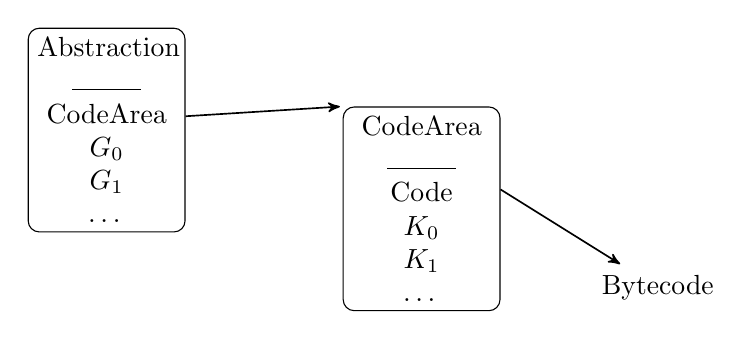
\begin{tikzpicture}[auto,every matrix/.style={ampersand replacement=\&,column sep=2cm,row sep=2cm},
                             to/.style={->,>=stealth',shorten >=1pt,semithick,font=\sffamily\footnotesize}]
  \node[block](abstraction) at (0,0) {Abstraction\\\line(1,0){25}\\
                             CodeArea\\
                             $G_0$\\
                             $G_1$\\
                             \dots\\};
  \node[block](codearea) at (4,-1) {CodeArea\\\line(1,0){25}\\
                             Code\\
                             $K_0$\\
                             $K_1$\\
                             \dots\\};
  \node[auto](bytecode) at (7,-2){Bytecode};

  \draw[to]  (abstraction.east)+(0,5pt) -- (codearea.north west);
  \draw[to]  (codearea.east)+(0,7pt)  --   (bytecode);
\end{tikzpicture}
\caption{Internals of the virtual machine}
\label{fig:internal_virtual_machine}
\end{figure}
Capturing the global variables at the abstraction level is what provides
closures: a procedure captures the environment it was defined in.
The CodeArea is not stored in the abstraction itself, but is referenced from
it, simply because the same CodeArea can be referenced from multiple
abstractions. The example from \cite{CTMCPFigs} in
Figure~\ref{fig:code_area_sharing} illustrates this.

% reference: http://www.info.ucl.ac.be/~pvr/bookfigures/fig3_8.oz

\begin{figure}[h]
\begin{lstlisting}
   fun {Sqrt X}
      fun {Improve Guess}
        (Guess + X/Guess) / 2.0
      end
      fun {GoodEnough Guess}
        {Abs X-Guess*Guess}/X < 0.00001
      end
      fun {SqrtIter Guess}
         if {GoodEnough Guess} then Guess
         else
            {SqrtIter {Improve Guess}}
         end
      end
      Guess=1.0
   in
      {SqrtIter Guess}
   end
\end{lstlisting}
\caption{Functions sharing the same CodeArea}
\label{fig:code_area_sharing}
\end{figure}

The method Sqrt computes the square root of a number by Newton's method. Each time Sqrt is
called, it defines three local functions. The two first reference the variable
X, which is a global variable for them, and which has probably a different
value at each call of Sqrt. However, the code area for each function is the
same for every call of Sqrt, and the virtual machine can simply create a new
abstraction referencing the already existing code area and defining the global
it needs.  Often, code areas are created at compile time, and the abstractions at run time.

If we have 2 simultaneous calls to Sqrt, for example {Sqrt 2} and {Sqrt 5}, we
would end up with the structure of Figure~\ref{fig:blurps} 
in the virtual machine.


\begin{figure}[h]
  \centering
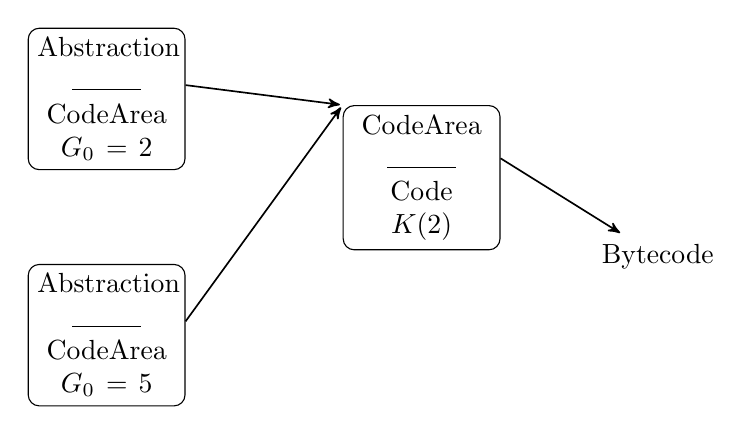
\begin{tikzpicture}[auto,every matrix/.style={ampersand replacement=\&,column sep=2cm,row sep=2cm},
                             to/.style={->,>=stealth',shorten >=1pt,semithick,font=\sffamily\footnotesize}]
  \node[block](abstraction) at (0,0) {Abstraction\\\line(1,0){25}\\
                             CodeArea\\
                             $G_0=2$\\
                             };
  \node[block](codearea) at (4,-1) {CodeArea\\\line(1,0){25}\\
                             Code\\
                             $K(2)$\\
                             };
  \node[auto](bytecode) at (7,-2){Bytecode};

  \node[block](abstraction2) at (0,-3) {Abstraction\\\line(1,0){25}\\
                             CodeArea\\
                             $G_0=5$\\
                             };

  \draw[to]  (abstraction.east)+(0,5pt) -- (codearea.north west);
  \draw[to]  (abstraction2.east)+(0,5pt) -- (codearea.north west);
  \draw[to]  (codearea.east)+(0,7pt)  --   (bytecode);
\end{tikzpicture}
\caption{Multiple Abstractions referring to the same CodeArea}
\label{fig:blurps}
\end{figure}


\section{Target Language}
The compiler generates code that can be passed to the assembler targeting the
virtual machine. This assembler language has solid support for the virtual
machine concepts as we will see. Appendix~\ref{appendix:opcodes} gives a reference list of
the opcodes available.

The core of the virtual machine is the emulator loop which interprets the bytecode. This loop is found in the file
\lstinline!emulate.cc! of the virtual
machine \cite{Moz2vmsrc} \footnote{http://git.io/5CcN2A}.

The assembler accepts an Oz list of instructions that are Oz tuples. This list
of opcodes is actually further transformed by
the assembler before it gets its definitive form and is fed to the virtual
machine.                                             

One transformation applied by the assembler is to translate generic operations
on register to operations specific to the registers manipulated. 

For example, we will present the \lstinline!move(src dst)! opcode taking a
source register and a destination register. This opcode is actually
specialised according to the source and destination register types. Source
register can be X, Y, G or K registers. Destination registers can be 
X or Y registers. As a consequence, \lstinline!move! is actually translated into
8 specialised operations. The resolution is done by the
assembler with a function
\lstinline!ResolveOverload! \cite{Moz2src}\footnote{http://git.io/XLk5wQ} 
which will actually resolve all overloaded opcodes that will be covered in this section. 

\subsection{Register Operations}\label{sec:intro:opcode:registers}
Registers access instructions are proper to each kind of register. To access the nth G X Y
registers, the instruction will respectively be \lstinline!g(n)!,
\lstinline!x(n)!, \lstinline!y(n)!. 

K registers are used to store constants. The assembler abstracts away the actual indexing of K registers. It expects values in \lstinline!k(V)! tuples, and assigns indices to K registers itself. The constant 2 will thus appear in the code as
\lstinline!k(2)!, the constant record \lstinline!r(a b c)! is denoted in the
code as \lstinline!k(r(a b c))!.


As mentioned earlier, Y registers are persisting for the lifespan of the current frame. Their number has to be determined when the frame is created, and all needed Y registers are allocated at once with the instruction \lstinline!allocateY(n)! where n is the number of Y registers used in this frame.
Y registers are deallocated when their owning frame is disposed of, i.e. upon exectution of one of \lstinline!return!, \lstinline!tailCall! or \lstinline!tailSendMsg!.

X registers are work registers, and if a value in an X register needs to be accessed several time across calls, it has to be saved in a Y register. This is done with a move instruction: \lstinline!move(source_reg destination_reg)!.
As mentioned earlier, source
can be  X, Y, G or K registers. Destination can be X or Y registers.

Unification is supported with the instruction \lstinline!unify(LHS RHS)! where
\lstinline!LHS! and \lstinline!RHS! are  X, Y, G, or K registers.
Internally, and because unification is commutative, this does not result in 16 but 10 specialised opcodes. For example,
\lstinline!moveXY! is defined, but not its mirror operator \lstinline!moveYX!.
It is the assembler's \lstinline!ResolveOverload! function that will pick the
available specialised operator and possibly switch the arguments order.

Two consecutive \lstinline!move! operations on registers X and/or Y registers are transformed by the assembler in
a \lstinline!moveMove! operation, transforming 
\begin{lstlisting}
   move(s1 d1) move(s2 d2)
\end{lstlisting}
 into
 \begin{lstlisting}
   moveMove(s1 d1 s2 d2)
 \end{lstlisting}

Four different situations can occur as both
source and destination can be X or Y registers resulting in 4
specialised operations \lstinline!moveMoveXYXY!, \lstinline!moveMoveYXYX!, \lstinline!moveMoveYXXY!,
\lstinline!moveMoveXYYX!.


\subsection{Variables}\label{sec:opcode:variables}
The opcode \lstinline!createVar(R)! assigns to register \lstinline!R!, which is
an X or Y register, a new unbound variable. The assembler also translates it to
\lstinline!createVarX! and \lstinline!createVarY!.

\lstinline!createVarMove(r(i) x(j))! is an opcode that will assign an unbound variable to
register \lstinline!r(i)! (X or Y), immediately followed by a
\lstinline!move! to register \lstinline!x(j)! (always an X register). This is very
handy when an unbound variable is passed as argument to a procedure, to be
reused after the call, as in

\begin{lstlisting}
   {MyProc ?R}
   {Show R}
\end{lstlisting}

The variable \lstinline!R! has to be in a Y register to be reused after the
call, but it has to be passed as argument to the call in an X register.
\lstinline!createVarMove! does both operations in one opcode.
Again, \lstinline!createVarMove! is actually specialised in
\lstinline!createVarMoveX! or \lstinline!createVarMoveY! if the first register is respectively an X or a Y register.


\subsection{Jumps}\label{sec:opcode:jumps}
Code positions can be identified by labels, which need to be atoms or names. A label \lstinline!L! is encoded in the code as a tuple \lstinline!lbl(L)!. 
Labels are required for jumps in the code. 
Jumps will move the execution to the label they have as argument. For example \lstinline!branch(endLabel)! will jump to the position in the code identified by the label \lstinline!endLabel!.

Conditional jumps will look at the value in an X register, and if this value is
not true, it will jump to the code at the label it was given. That instruction
also takes a label locating error handling code. Here is an example of
conditional jump that will look at the value in X register 0:
\begin{lstlisting}
   condBranch(x(0) elseLabel errorLabel)
\end{lstlisting}
If the value in x(0) is
true, it continues execution. If it is false it jumps to the position in the
code identified by the label \lstinline!elseLabel!. If an error occurs in the
test, it jumps to the label \lstinline!errorLabel!. This is illustrated in Figure~\ref{fig:target:condBranch}.
If the value in register \lstinline!x(0)! is not tested successfully as a
boolean, execution will jump to \lstinline!lbl(1)! and raise an exception. If
the condition (the value in \lstinline!x(0)!) is true, the code will execute
\lstinline!{Show 'true'}!, else it will execute \lstinline!{Show false}!.

\begin{figure}[ht]
\begin{lstlisting}

                condBranch(x(0) 2 1)
                move(k('true') x(0))
                call(k(<P/1 Show>) 1)
                branch(3)
lbl(1)          move(k(badBooleanInIf) x(0))
                tailCall(k(<P/1 Exception.raiseError>) 1)
lbl(2)          move(k('false') x(0))
                call(k(<P/1 Show>) 1)
lbl(3)          return

\end{lstlisting}
\caption{Conditional branch example}
\label{fig:target:condBranch}
\end{figure}



\subsection{Calls}\label{sec:opcode:calls}
Calls can be made with \lstinline!call(R Args)!, where R is an 
X, Y, G or K register.
identifying what to call (procedure or builtin) and Args is the number of
arguments passed to the callee. As per the calling convention of the vm bytecode, the arguments of the call have to be placed in the X registers from 0
to Args-1 with move instructions before the call. The complete code for a call to a callee
located in register Y 3 with three arguments which values come from Y registers
4 to 6 will thus be of the form illustrated in
Figure~\ref{fig:opcodes:callexample}.
\begin{figure}[h]
\begin{lstlisting}
   move(y(4) x(0))
   move(y(5) x(1))
   move(y(6) x(2))
   call(y(3) 3)
\end{lstlisting}
\caption{Opcodes for a call}
\label{fig:opcodes:callexample}
\end{figure}


A call done as last instruction of an abstraction should be made with the
\lstinline!tailCall! instruction, as this lets the virtual machine optimise the
execution (see below). It has the exact same arguments as the call instruction, only the
name of the instruction differs: \lstinline!tailCall(Callee Args)!.

\lstinline!call! starts by creating a new frame on the stack with the currently
running abstraction/code area, the program counter, and the Y registers.
\lstinline!tailCall! instead frees the Y registers.
After that, the current abstraction and its code area are replaced by the callee
and its code area.


A builtin is called with \lstinline!callBuiltin(k(BI) Args)!, where
\lstinline!BI! must be a builtin (i.e. \lstinline!{IsBuiltin BI} == true!).

\lstinline!callBuiltin! always takes the builtin to call in a K register, but it is nonetheless specialised in different operations with 0 to 5
arguments or with an arbitrary number of arguments N. These are called
\lstinline!callBuiltinX! where X is one of \lstinline!0 1 2 3 4 5 N!.

\lstinline!return! cleans the Y registers and pops the top frame on the stack.


\subsection{Records}\label{sec:opcode:records}
Without being exhaustive, here is a reminder of the record concept in Oz. 

A record is defined by \lstinline!Label(F1:V1 F2:V2)! where the label and features
(\lstinline[mathescape]!$F_i$!) can be an integer, an atom or a variable, and the values
(\lstinline[mathescape]!$V_i$!) can any expression. Features can be left out, in which case they are implicitly assigned increasing values from 1.

At the virtual machine and compiler level, the arity of a record is made of its
label and features.
A tuple is a record whose features are consecutive integers starting from 1. 
In an abuse of language and only when no confusion is possible, we will
sometimes refer to a feature's value simply as ``feature''. This simplifies the
text without adding confusion, especially in the case of tuples where features
are known to be numeric.

Records, tuples and cons are directly supported by the virtual machine, handling each of these particularly to ensure performance and efficiency.
A record of arity Arity, with NumberOfFeatures features is unified with 
DestinationReg (an X, Y, G or K register) with this instruction:
\begin{lstlisting}
   createRecordUnify(k(Arity) NumberOfFeatures DestinationReg)
\end{lstlisting}
which has to be followed by instructions to fill the features with their respective values:
\begin{lstlisting}
   arrayFill(Reg)
\end{lstlisting}
where Reg is the register corresponding to the feature's value\footnote{\lstinline!arrayFill! might be renamed in \lstinline!structFill! in the future}.
The arity is supported by the virtual machine and includes the label and features without their respective values.

There are two special cases of records that are handled specifically by the virtual machine.
A cons is a record with label \lstinline!'|'! and with only 2 features numbers 1
and 2 and is initialised by:
\begin{lstlisting}
   createConsUnify(DestinationReg)
\end{lstlisting}
Again, this instruction has to be
followed by \lstinline!arrayFill! instructions, two in this particular case.
A tuple is a record with all consecutive numeric features from 1. It is initialised with 
\begin{lstlisting}
   createTupleUnify(k(Label) NumberOfFeatures DestinationReg)
\end{lstlisting}
and followed by \lstinline!arrayFill! instructions.

Each of these instructions have a \lstinline!Store! version (for example
\lstinline!createConsStore!) with the same arguments. This opcode stores the
record created in the destination register which in this case must be an X
or Y register, instead of unifying former with the entity created.

\subsection{Procedures}\label{sec:opcode:procedures}
A procedure is represented by what is called an abstraction (see Section
\ref{sec:vm:abstractions}), which is created and unified with the contents of register
\lstinline!DestinationReg! with
\begin{lstlisting}
   createAbstractionUnify(k(CodeArea) GlobalsCount  DestinationReg)
\end{lstlisting}
\lstinline!CodeArea! is the assembled body of the procedure (see Section
\ref{sec:codegen:procedures} for details). \lstinline!GlobalsCount! identifies
how many references to global variables this abstraction holds. It is the number
of \lstinline!arrayFill! instructions that will follow to initialise those global variables
that the abstraction can access in G registers numbered from 0. The first
\lstinline!arrayFill! instruction will set the value of \lstinline!g(0)!, the
second the value of \lstinline!g(1)!,
\ldots

Figure~\ref{fig:opcodes:procedures:example} lists the Oz code we will analyse.

\begin{figure}[ht]
\begin{lstlisting}
local
  A B P
in
  A=1           % in register X 0
  B=2           % in register X 1
  proc {P}      % in register Y 0
    {Show A+B}  % A and B are globals for P
  end           % access in g(0) and g(1) resp.
end
\end{lstlisting}
\caption{Oz code example for opcodes generation}
\label{fig:opcodes:procedures:example}
\end{figure}


As noted in the code comments, we suppose, the compiler having done its work of
registers allocation, variables \lstinline!A! and \lstinline!B! are stored in
registers \lstinline!x(0)! and \lstinline!x(1)!
respectively, that the abstraction for procedure \lstinline!P! is stored in register \lstinline!y(0)!
, and that \lstinline!P! accesses the values of \lstinline!A! and \lstinline!B!
via the registers \lstinline!g(0)! and \lstinline!g(1)!
respectively.
The body having been assembled and stored in the constant value
\lstinline!CodeArea!, this
will lead to the code in Figure~\ref{fig:opcodes:procedures:result} to be passed
to the assembler.
\begin{figure}[ht]
\begin{lstlisting}
   createAbstractionUnify(k(CodeArea) 2  y(0))
   arrayFill(x(0))
   arrayFill(x(1))
\end{lstlisting}
\caption{Opcodes generated for example Oz code}
\label{fig:opcodes:procedures:result}
\end{figure}

\lstinline!createAbstractionStore! is used similarly to the records'
\lstinline!Store! instructions.

\subsection{Pattern Matching}
The target language supports pattern matching with the instruction
\begin{lstlisting}
  patternMatch(Reg PatternMatchRecord)
\end{lstlisting}
where \lstinline!Reg! is the X, Y or G register containing the value to test, and
\lstinline!PatternMatchRecord! is a record specifying the patterns and their
respective jump address in case of a match.
Figure~\ref{fig:target:ozcase} gives a simple Oz case instruction, and Figure~\ref{fig:target:case} lists the generated opcodes.
Section~\ref{sec:arch:codegen:case} covers pattern matching and the \lstinline!patternMatch! instruction thoroughly.
 
\begin{figure}[ht]
\begin{lstlisting}
   case R
   of l(1 2) then
      {Show 'l'}
   [] rec(a b) then
      {Show 'rec'}
   else
      {Show 'else'}
   end
   ...
\end{lstlisting}
\caption{Example \lstinline!case! instruction}
\label{fig:target:ozcase}
\end{figure}

\begin{figure}[ht]
\begin{lstlisting}
                patternMatch(x(0) k((l(1 2)#6)#(rec(a b)#7)))
                branch(5)
lbl(6)          move(k(l) x(0))
                call(k(<P/1 Show>) 1)
                branch(3)
lbl(7)          move(k(rec) x(0))
                call(k(<P/1 Show>) 1)
                branch(3)
lbl(5)          move(k('else') x(0))
                call(k(<P/1 Show>) 1)
lbl(3)          ...
\end{lstlisting}
\caption{Opcodes for the example \lstinline!case! instruction}
\label{fig:target:case}
\end{figure}




\subsection{Exceptions}
There is an opcode to setup an exception handler and jump to a label:
\begin{lstlisting}
  setupExceptionHandler(DestLabel)
\end{lstlisting}
If the code executed from \lstinline!DestLabel! raises an exception before  the exception handler
is removed with \lstinline!popExceptionHandler!, the execution will jump to the
opcode following the instruction \lstinline!setupExceptionHandler!.

Figure~\ref{fig:opcodes:exception:oz} gives a simple example of Oz code
handling exceptions, and Figure~\ref{fig:opcodes:exception:result} gives an
idea of corresponding opcodes. The opcodes corresponding to
\lstinline!ExceptionHandlingOpCodes! and more detailed examples are given in
Section \ref{sec:arch:codegen:exceptions}.
\begin{figure}[ht]
\begin{lstlisting}
   try
      {Show 1}
   catch E then
      {Show 'catched exception'}
   end
\end{lstlisting}
\caption{Oz code handling exceptions}
\label{fig:opcodes:exception:oz}
\end{figure}



\begin{figure}[ht]
\begin{lstlisting}
    
                   setupExceptionHandler(1)
                   ExceptionHandlingOpCodes
                   branch(2)
   lbl(1)          move(k(1) x(0))
                   call(k(<P/1 Show>) 1)
                   popExceptionHandler
   lbl(2)          return
\end{lstlisting}
\caption{Opcodes handling exceptions}
\label{fig:opcodes:exception:result}
\end{figure}


\subsection{Skip}
\lstinline!skip! is a no-op opcode, that is actually dropped by the assembler.
It is however available to ease the generation of the opcodes having some parts
optional. Rather than testing if the opcodes sublist is empty before including
it in the whole program's opcodes list, it is possible to generate it in every
case: for the situation in which no operation is needed, a \lstinline!skip! opcode will be
issued.
If the vm loop encounters a \lstinline!skip! opcode, it does nothing and goes to the next opcode.






\section{Compiler input}\label{section:compilerinput}
The compiler takes as input the AST in the form of Oz records \cite{AST}, and generates opcodes sent to the assembler. 
This section will present and describe the records received from the parser and
their corresponding Oz form.
\subsection{Position in source code}
Most records have the corresponding position in the source code available in
their last feature, encoded in a record of the form:
\begin{lstlisting}
pos(File Linebegin Columnbegin Fileend Lineend Columnend)
\end{lstlisting}
The position of each instruction has to trickle through all transformations so meaningful error messages can be given to the programmer in case of error.
Most of the nodes in the AST include the position of their instruction in the
source code.

For clarity and brevity, in the examples of AST included in this document, the
positions will always be represented by the featureless record \lstinline!pos!
or a variable named \lstinline!Pos!. 
\subsection{Literals}
The basic data type described in this section are the simplest node found in the AST as they have no children and are always leafs of the AST.
These are the basic data types with their corresponding tuples in the AST:
\begin{description}
  \item[integers] \lstinline!fInt(Val Pos)!
  \item[floats] \lstinline!fFloat(Val Pos)!
  \item[atoms] \lstinline!fAtom(value position)!
\end{description}

\lstinline!fAtom! are also used to place \lstinline!unit!, \lstinline!true! and
\lstinline!false! in the AST.

\subsection{Identifiers}\label{sec:input:identifiers}
An identifier is denoted by a tuple \lstinline!fVar(Ident Pos)! in the AST,
where \lstinline!Ident! is the text of the identifier represented as an atom.

\subsection{Unification}
A unification is found in a tuple \lstinline!fEq(LHS RHS Pos)!.
\lstinline!A=3! results in 
\lstinline!fEq(fVar(A pos) fInt(3 pos) pos)!.

\subsection{Instructions sequence}
A sequence of instructions is wrapped in fAnd records, the first feature being usually one instruction, the second feature being an fAnd if more than one instruction follows,  or a single instruction. 
%The code also handles the case when the two features are \lstinline!fAnd! records.
Here is an example of three unifications and the corresponding AST:\\
\begin{tabular}{ p{0.3\textwidth} p{0.8\textwidth} }
  \begin{lstlisting}
    A=1
    B=2
    C=3
  \end{lstlisting}
&
  \footnotesize{
  \begin{lstlisting}
  fAnd( fEq (fVar (A pos) fInt (1 pos))
        fAnd(fEq (fVar(B pos)) fInt(2 pos) 
             fEq(fVar(C pos) fInt(3 pos))))
  \end{lstlisting}
  }
\end{tabular}

\subsection{Local}\label{sec:input:flocal}
\lstinline!local..in..end! are represented in the AST by tuples of the form
\begin{lstlisting}
   fLocal(Declarations Body Pos)
\end{lstlisting}
where \lstinline!Declarations! and
\lstinline!Body! are both AST subtrees. 
Figure~\ref{fig:input:decls_oz} shows Oz code declaring the three variables
\lstinline!A!, \lstinline!B!
and \lstinline!C!, and bounding variable \lstinline!A! with integer
\lstinline!1!. The AST corresponding to this Oz code is shown in
Figure~\ref{fig:input:decls}.

\begin{figure}
\begin{lstlisting}
local
  A B C
in
  A=1
end
\end{lstlisting}
\caption{Declaration of 3 variables}
\label{fig:input:decls_oz}
\begin{lstlisting}
fLocal(
       fAnd(
            fVar(A pos) 
            fAnd(
                 fVar(B pos) 
                 fVar(C pos) 
                 pos) 
            pos) 
       fEq( 
            fVar(A pos) 
            fInt(1 pos) ))
\end{lstlisting}
\caption{AST for the the code in Figure~\ref{fig:input:decls_oz}}
\label{fig:input:decls}
\end{figure}


\subsection{Procedures}\label{sec:input:procedures}
\subsubsection{Definitions}
Procedures are found in records of the form 
\begin{lstlisting}
   fProc(Name Arguments Body Flags Pos) 
\end{lstlisting}
where the \lstinline!Arguments! and \lstinline!Body! features are AST subtrees. 
Figure~\ref{fig:input:oz_procedure_def} and Figure~\ref{fig:input:ast_procedure_def} show a small procedure definition and its corresponding AST.
\begin{figure}[ht]
\begin{lstlisting}
   proc {P A1 A2}
      {Show A1}
      {Show A2}
   end
\end{lstlisting}
\caption{Oz procedure definition}
\label{fig:input:oz_procedure_def}

\begin{lstlisting}
   fProc(
      fVar('P' pos)
      [
        fVar('A1' pos)
        fVar('A2' pos)]
      fAnd(
         fApply(
            fVar('Show' pos)
            [fVar('A1' pos)]
            pos)
         fApply(
            fVar('Show' pos )
            [fVar('A2' pos)]
            pos))
      pos)
\end{lstlisting}
\caption{AST of the Oz procedure definition}
\label{fig:input:ast_procedure_def}
\end{figure}



\subsubsection{Calls}
Procedure calls are found in records of the form 
\lstinline!fApply(Proc Arguments Pos)!. 
Example:

\begin{lstlisting}
  {Compute 1 2 3}
\end{lstlisting}

will result in the AST portion:
\begin{lstlisting}
fApply(
       [ fVar(Compute pos)
         fInt(1 pos)
         fInt(2 pos)
         fInt(3 pos)
       ])
\end{lstlisting}

\subsection{Functions}\label{sec:input:functions}
Function definitions are found in the AST in \lstinline!fFun! tuples, with the
same features found in \lstinline!fProc! records. Functions are simply
procedures that implicitly return exactly one value. This similarity between
functions and procedures can be seen in their similar AST for definitions and
calls. It will be exploited later on to merge both forms of AST
into one.
However, only functions can be marked as lazy as in \lstinline!fun lazy {F N} .. end!. This lazy marker is translated in a flag.
\subsubsection{Definitions}
Function definitions are found in records fFun(Name Arguments Body Flags Pos). The features are identical to the procedure definition.
\subsubsection{Calls}
The calls of functions are identical to the call of procedures as they are found in fApply.

\subsection{Operators}\label{sec:input:operators}
Operators are parsed as records of the form
\begin{lstlisting}
   fOpApply(Operator Args Pos)
\end{lstlisting}
 whose first feature is the operator to
apply, its second feature being the list of operands. It also has a position
record as third feature. For example
\lstinline!5+2! is parsed as displayed in Figure~\ref{fig:opexample}.
\begin{figure}[h]
\begin{lstlisting}
      fOpApply(
         '+'
         [
           fInt(5 pos)
           fInt(2 pos )
         ]
         pos
      )
\end{lstlisting}
\caption{AST for \lstinline!5+2!}
\label{fig:opexample}
\end{figure}

\subsection{Nesting marker \$}\label{sec:input:nestingmarker}
In Oz, some statements can be transformed in expressions by the use of the
\lstinline[mathescape]!$\$$!
marker. This marker is found in the AST as a tuple \lstinline!fDollar()! with a unique
feature: its position.
The statements that can be transformed in expressions are
\begin{itemize}
  \item Function, Procedure, Functor and Class declarations. \\For example
    \lstinline[mathescape]!X=fun{$\$$ A B} .. end!
  \item A call to a procedure having the nested procedure in one of the pattern positions of its arguments.
\end{itemize}
The pattern positions \lstinline!PP! of an argument being the union of 
\begin{itemize}
  \item the argument itself
  \item if it is a record of the form \lstinline!l(f1:v1 ... fn:vn)!, $PP(v1) \cup ... \cup PP(vn)$.
\end{itemize}

\subsection{Cells}\label{sec:input:cells}
\subsubsection{Assignation}
A new value can be stored in a cell with this Oz code: \lstinline!Cell:=Val!. This code will result in 
this tuple in the AST: \lstinline!fColonEquals(Cell Val Pos)!. 
\subsubsection{Read}
The value stored in a cell can be access with the \lstinline!@! operator, as is
\lstinline!@Cell!, which results in this tuple in the AST: 
\lstinline!fAt(Cell Pos)!
\subsection{Records}\label{sec:input:records}

Records are present in the AST as tuple with label \lstinline!fRecord!. Its
label is the first feature, and the second feature is the list of feature-value
pairs. If no explicit feature was specified, the entry in the list is simply the value.
If an explicit feature was specified, the entry in the list is a tuple \lstinline!fColon!, with the
first feature being the feature and second feature being the value. All this
will become much clearer with the following examples.

Figure~\ref{fig:recordsast} displays the AST corresponding to the record \lstinline!rec(f1:v1 f2:v2)!. We see that the label (rec) is an atom located in an \lstinline!fAtom! tuple. The pairs of features and their respective values are wrapped in fColon.

\begin{figure}[h]
\begin{lstlisting}
   fRecord(
      fAtom(rec pos)
      [
       fColon(
         fAtom(f1 pos)
         fAtom(v1 pos))
       fColon(
         fAtom(f2 pos)
         fAtom(v2 pos))])
\end{lstlisting}
\caption{Record AST}
\label{fig:recordsast}
\end{figure}


When the feature is not explicitly given, the item in the list of features and their respective values is simply the value. Figure~\ref{fig:astfeature} is the AST of \lstinline!rec(v1 f2:V2)!. The first item in the list is simply an atom, the value of the first feature. Note that the value of the feature f2 is a variable in this case.

\begin{figure}[h]
\begin{lstlisting}
   fRecord(
      fAtom(rec pos)
      [
       fAtom(v1 pos)
       fColon(
          fAtom(f2 pos)
          fVar(V2 pos))])
\end{lstlisting}
\caption{AST for record with implicit feature}
\label{fig:astfeature}
\end{figure}



\subsection{Wildcards}\label{sec:input:wildcard}
Oz syntax allows to put a wildcard \lstinline!_! in the location of a value we want to ignore, for example in calls and records pattern matching. These markers are present in the AST in the form of a tuple \lstinline!fWildcard(Pos)!.
Ignoring the value returned by a function is thus written \lstinline!_={F N}!. 
This allows the user to not declare variables he wouldn't use anyway, which would in addition raise a warning about a variable used only once\ldots

Pattern matching is covered extensively in Section \ref{sec:input:patternmatching}.

\subsection{Threads}
Thread instructions are present in the AST in the form of tuples with label \lstinline!fThread!, and with two features: the body of the thread, and its position in the source code:
\begin{lstlisting}
   thread Body end
\end{lstlisting}
results in
\begin{lstlisting}
   fThread(Body pos)
\end{lstlisting}
\subsection{Locks}\label{sec:input:locks}
Oz enables the programmer to protect a critical section with a lock previously created with \lstinline!L={NewLock}!:
\begin{lstlisting}
   lock L then
      % critical section
   end
\end{lstlisting}

This code results in a tuple \lstinline!fLockThen! in the AST, with 3 features: the lock L,
the body of the critical section, and the position in the code:
\lstinline!fLock(L Body Pos)!.

\subsection{If then else}
The \lstinline!if..then..else! construct is put in a tuple:
\begin{lstlisting}
   fBoolCase( Condition ThenCode ElseCode)
\end{lstlisting}
The else part is optional in Oz. In this case, ElseCode is a tuple \lstinline!fNoElse(pos)! in the AST.

\subsection{Short-circuit boolean combinators}\label{sec:input:booleancombinations}
The boolean conjunction operation in Oz is represented by the keyword \lstinline!andthen!. Such a conjunction is present in the AST in the form of a tuple 
\begin{lstlisting}
   fAndThen(First Second)
\end{lstlisting}
where first and second must be expressions with a boolean value.
The boolean disjunction operation is done using the keyword \lstinline!orelse!, present in the AST in the form of a tuple \lstinline!fOrElse(First Second)!.

\subsection{Case Instruction and Pattern Matching}\label{sec:input:patternmatching}
The Case instruction in Oz is of the following form where optional parts are enclosed in double square brackets ([[ ]]).
\begin{lstlisting}
   case Value                           % _
   of Pattern1 [[andthen Guards1]] then %  \____ This is a clause
     Code1                              % _/
   [] Pattern2 [[andthen Guards2]] then
     Code2
   ..
   [[else
     ElseCode]]
   end
\end{lstlisting}
This ends up in the AST in a tuple of the form 
\begin{lstlisting}
   fCase(Value Clauses ElseCode pos)
\end{lstlisting}
\lstinline!Clauses! is a list of tuples each representing one clause and containing the clause' pattern, guards and code. We will analyse these further below.
The else part of the instruction is optional. If no else is provided, then ElseCode in the AST is a tuple \lstinline!fNoElse(pos)!.

A clause with no guards is present in the AST in the form of a tuple \lstinline!fCaseClause(Pattern Body)!. \lstinline!Pattern! can be a constant value (integer, string, record, \ldots), present in the AST as described earlier. It can also be a record where a feature's value is not a constant but a variable (in a \lstinline!fVar(Name pos)! record as described in section \ref{sec:input:identifiers}). In case of a match of the constant feature values in the pattern, this declares said variable and assigns the value of the corresponding feature in the value the pattern is tested against. Here is an example:
\begin{lstlisting}
  R=lab(a b c d)
  case R
  of lab(a B c d) then
    {Show B}  % B's value is b
  end
\end{lstlisting}
Features of a record in a pattern can also have the wildcard \lstinline!_! as value, represented in the AST as described in section \ref{sec:input:wildcard}.

The pattern can also be or contain an open record specifying only a subset of features which should match, as in the following example:
\begin{lstlisting}
  R=lab(a b c d)
  case R
  of lab(3:c 4:_ ...) then
    % Code for record matching pattern
  end
\end{lstlisting}
The syntax for an open record pattern is the same as for a record pattern, except that subsequent features that should be ignored are replaced by \lstinline!...!. Also in the AST an open record is very similar to a record. Only the label changes to \lstinline!fOpenRecord!, and only the specified features are present in the AST, the \lstinline!...! being absent from the AST. Here is an example of an open record:
\lstinline!lab(a b ...)! 
and its AST representation:
\begin{lstlisting}
   fOpenRecord(
      fConst(lab pos)
      [
       fColon(
          fConst(1 pos)
          fConst(a pos))
       fColon(
          fConst(2 pos)
          fConst(b pos))])
\end{lstlisting}

Records and open records can of course be nested.

A clause with guards is present in the AST in the form of a tuple
\begin{lstlisting}
   fSideCondition(Pattern Decls Guards Pos)
\end{lstlisting}
where \lstinline!Pattern!
is as above,
and \lstinline!Guards! is simply the AST of the code of the guard (without the \lstinline!andthen! introducing the guard).
\lstinline!Guards! must be an expression with a boolean value, possibly using
the short-circuit boolean combinators of section \ref{sec:input:booleancombinations}.

\lstinline!Decls! is the declarations introduced by the guards, as the variable \lstinline!X! in the code of Figure~\ref{fig:guardsdecls}.
When there are no declarations, the value is \lstinline!fSkip(pos)!

\begin{figure}[h]
\begin{lstlisting}
   case Foo
   of bar(F) andthen X = F+4 in X > 0 then 
      {Show X}
   end
\end{lstlisting}
\caption{Guards declarations}
\label{fig:guardsdecls}
\end{figure}


Variables can also be used in patterns for their value, and not as a new capture
declaration. This is done by prefixing the variable with an exclamation mark.
Here is an example:

\begin{lstlisting}
A=a
case V
of rec(A b c) then
   % matches rec(_ b c), i.e. all records with label rec, second feature 
   % value b, third value c, with A being a new capture variable
[] rec(!A b c) then
   % only matches rect(a b c)
end
\end{lstlisting}

An escaped variable ends up in the AST as wrapped in an \lstinline!fEscape!
tuple. \lstinline$!A$ appears in the AST as \lstinline!fEscape( fVar(A pos) pos)!.
\nav{The next transformation of \lstinline!fEscape! nodes is done by the Namer,
see Section \ref{sec:arch:namer:patternmatching}.}

Oz pattern matching also support what is called pattern conjunction, enabling to
capture the value of a subexpression of the pattern as illustrated in this example:
\begin{lstlisting}
   case V 
   of rec(I=inner(a b ...)) then
   ...
   end
\end{lstlisting}

In the clause'code, the variable \lstinline!I! will have the value of the inner record.
These pattern conjunctions are present in the AST in \lstinline!fEq! tuples just 
like unification instructions.
Note that just like unifications (and unlike \lstinline!local..in..end!), the variable implicitly declared can be at the
left as well as at the right side of the equal sign. So the pattern
\lstinline!rec(V=inner(a b ...))! is equivalent to \lstinline!rec(inner(a b ...)=V)!
And also like in unification, the capturing side can be a pattern, it doesn't
have to be a single variable.

\begin{figure}[h]
\begin{lstlisting}
   case {GetToken}
   of unit then
      skip
   elseof S then
      {Handle S}
   end
\end{lstlisting}
\caption{\lstinline!elseof! construct}
\label{fig:input:elseof}
\end{figure}



\subsection{Classes}
Analysing classes is best illustrated by an example of Oz code:

\begin{lstlisting}
   class C
      meth init skip end
      meth hello(A1)
         {Show 'hello'}
         {Show A1}
      end
   end
\end{lstlisting}
which results in this AST:
\begin{lstlisting}

   fClass(
      fVar('C' pos )
      nil
      [
        fMeth(
           fAtom(init pos )
           fSkip(pos )
           pos)
        fMeth(
           fRecord(
              fAtom(hello pos )
              [
                fMethArg(
                   fVar('A1' pos )
                   fNoDefault)
              ])
           fAnd(
              fApply(
                 fVar('Show' pos )
                 [
                    fAtom(hello pos )
                 ]
                 pos)
              fApply(
                 fVar('Show' pos )
                 [
                    fVar('A1' pos )
                 ]
                 pos))
           pos)
       ]
      pos)
\end{lstlisting}

Class definitions are found in 
\lstinline!fClass(ClassVar SpecsList MethodsList Pos)!.
A method is found in a tuple \lstinline!fMeth(Signature Body Pos)!.
For methods without argument, \lstinline!Signature! is simply the method name.
In the example, this is illustrated by the \lstinline!init! method.
For methods with arguments, \lstinline!Signature! is the AST of a record whose label is the method name, and the
values in the record are the method arguments found in 
\lstinline!fMethArg(Var DefaultValue)!, where \lstinline!DefaultValue! is
\lstinline!fNoDefault! if none was provided.
This is illustrated by the method \lstinline!hello(A1)!.

The class of this example had no feature, attribute, parent or property defined, hence the empty
list as value of the second feature.
Both attribute and features are placed in this list. Attributes are placed in
\lstinline!fAttr(AttrsList)! tuples and features are placed in
\lstinline!fFeat(FeatsList)! tuples. Both these tuples have one feature whose
value is a list. Each attribute and feature corresponds to one item in its
respective list. If the attribute or feature has a default value, its
corresponding item is a record with label \lstinline!'#'! and two values: the
first is the name of the attribute or feature, the second is the default value.
If no default value is defined, the item in the list is simply the name of the
attribute or the feature.
Let's look at an example. A class with the following attributes and feature
definition
\begin{lstlisting}
      attr
         count:0
         state
      feat
         type:repeater
  
\end{lstlisting}
will have its list of attributes and features looking like this:
\begin{lstlisting}
      [
         fAttr(
            [ #( fAtom(count pos)
                  fInt(0 pos ))
              fAtom(state pos ) ]
            pos)
         fFeat(
            [ #(
                 fAtom(type pos )
                 fAtom(repeater pos )) ]
            pos)
      ]
\end{lstlisting}
The \lstinline!count! attribute is placed in a '\#' record, but not
the \lstinline!state! attribute.
All attributes are placed in one \lstinline!fAttr!
tuple, and all features in one \lstinline!fFeat! tuple.

This list also contains more information: the parents of the class, as well as
the properties of the class. 

The parents are located in \lstinline!fFrom(ParentsList)!. 
Here is an example from a class inheriting from classes \lstinline!A! and
\lstinline!B!. In Oz, this class will be defined by
\begin{lstlisting}
  class C from A B
    ..
  end
\end{lstlisting}
and this will result in this element in the list
\begin{lstlisting}
           fFrom(
              [ fVar('A' pos )
                fVar('B' pos )]
            pos)
\end{lstlisting}

The properties of a class are also present in that list, under \lstinline!fProp!
tuples. A class having the locking property would have this \lstinline!fProp! tuple:

\begin{lstlisting}
           fProp(
               [fAtom(locking pos)]
               pos)
\end{lstlisting}

When a class has the \lstinline!locking! property, a lock is implicitly created,
that can be used in a method with the \lstinline!lock! statement without
specifying the lock object, as this:

\begin{lstlisting}
   meth update(A)
      lock
         ..
      end
   end
\end{lstlisting}

This \lstinline!lock! instruction is put in the AST as a node
\lstinline!fLock(Body Pos)!. \nav{The next transformation to this node 
takes place in the desugar step described page \pageref{desugar:classes:lock}.}

Assignation to attributes can be done in two ways. The first has the same syntax
as cell updates, described in Section \ref{sec:input:cells}:
\begin{lstlisting}
  my_attr:=NewVal
\end{lstlisting}
and is found in the AST just as a cell update operation under a node
\lstinline!fColonEquals!.

The second uses the syntax \lstinline!<-!, as in:
\begin{lstlisting}
  my_attr<-NewVal
\end{lstlisting}
and is found in the AST under a node \lstinline!fAssign(LHS RHS pos)!.

\label{compilerinput:classes:headcapture}The method head can also be captured and made available to its body,as in 
\begin{lstlisting}
   meth echo(First ...)=H
      Body
   end  
\end{lstlisting}
At run time, the \lstinline!H! variable will give access to the message sent to the object, with the actual arguments list.
\begin{lstlisting}
               fMeth(
                  fEq(
                     fOpenRecord(
                        fAtom(echo pos )
                        [ fMethArg(
                              fVar('First' pos )
                              fNoDefault)])
                     fVar('H' pos )
                     pos)
                  BodyAST
                  Pos)
\end{lstlisting}

Method can also be defined as private by using a variable name as their label:
\begin{lstlisting}
   meth A(V)
      Body
   end
\end{lstlisting}
resulting in the AST in Figure~\ref{fig:privatemeth}.

\begin{figure}[h]
\begin{lstlisting}
   fMeth(
      fRecord(
         fVar('A' pos )
         [ fMethArg(
              fVar('V' pos )
              fNoDefault)]
      BodyAST
      pos)
\end{lstlisting}
\caption{Private method AST}
\label{fig:privatemeth}
\end{figure}

The method \lstinline!A! will be bound to a new name, only visible in the class
definition's scope (see Section \ref{sec:arch:namer:classes} for details).

Method can also have dynamic labels assigned, by escaping the variable holding
the label to use:
\begin{lstlisting}
  meth !A(V)
     Body
  end
\end{lstlisting}
The AST for a dynamic label assigned to a method is:
\begin{lstlisting}
    fMeth(
       fRecord(
          fEscape(
             fVar('A' pos)
             pos)
          [ fMethArg(
                fVar('V' pos)
                fNoDefault) ]
       BodyAST
       pos)

\end{lstlisting}

\subsection{Loops}
There are three forms of the \lstinline!for..in..do..end! statement, working
respectively on list, ranges, and C-like for loops conditions.
\subsubsection{Iterating over lists}
The Oz syntax is best illustrated by an example:
\begin{lstlisting}
   for Var in L do {Show Var} end
\end{lstlisting}
\lstinline!Var! is bound to each element of L in turn, and the code executed.
Hence this code will show all elements of the list L.

Multiple list can be iterated:
\begin{lstlisting}
   for I in L J in L2 do {Show I#J} end
\end{lstlisting}
but note that the iteration goes over the two zipped lists , and the loop ends once the
end of one of the list is reached. The number of times the body of the loop is
called is thus the number of elements of the smallest list.

The AST of the first \lstinline!for! example is displayed in Figure~\ref{fig:forlist}.
\begin{figure}[h]
\begin{lstlisting}
   fFOR(
      [forPattern(
           fVar('Var' pos )
           forGeneratorList(
              fVar('L' pos ))) ]
      fApply(
         fVar('Show' pos )
         [fVar('Var' pos)]
         pos)
      pos)
\end{lstlisting}
\caption{For loop iterating over list \lstinline!L!}
\label{fig:forlist}
\end{figure}


The first value in the \lstinline!fFor! tuple is the list of patterns, one
for each list. Each item of this list is a \lstinline!forPattern! tuple, with
its first value being the variable that will be available in the loop, and the
second value an \lstinline!fGeneratorList! tuple referencing the list over which to
iterate.
The second value in the \lstinline!fFor! tuple is the code to be executed for
each element of the list.

\subsubsection{Iterating over ranges}
Here is an example of a \lstinline!for! loop iterating over integers from 1 to 5
with a step of 2, resulting the execution of the body of the loop for integers 1
3 and 5:
\begin{lstlisting}
   for I in 1..5;2 do {Show I} end
\end{lstlisting}

\begin{lstlisting}
   fFOR(
      |(
         forPattern(
            fVar('I' pos )
            forGeneratorInt(
               fInt(1 pos )
               fInt(5 pos )
               fInt(2 pos )))
         nil)
      fApply(
         fVar('Show' pos )
         |(
            fVar('I' pos )
            nil)
         pos)
      pos)
\end{lstlisting}

The AST is very similar to the first loop form, only the
\lstinline!fGeneratorList! tuple is replaced by a \lstinline!forGeneratorInt!
tuple holding the specification of the range and step to use.

\subsubsection{C-style for loops}
Iterating over integers from 1 to 5 with a step of 2 can also be written in the C-style for loop:
\begin{lstlisting}
   for I in  1;I<4;I+1 do  {Show I} end
\end{lstlisting}
It takes a generator composed of 3 expressions: \lstinline!E1;E2;E3! where
\lstinline!E1! is the start value, \lstinline!E2! is the test condition, the
looping continuing as long at it evaluates to true, and \lstinline!E3! is the
next value's expression.
It is found in the AST illustrated in Figure~\ref{fig:forc}.
\begin{figure}[h]
\begin{lstlisting}
   fFOR(
      [ forPattern(
           fVar('I' pos )
           forGeneratorC(
              fInt(1 pos )
              fOpApply(
                 '<'
                 [ fVar('I' pos )
                   fInt(4 pos ) ]
                 pos)
              fOpApply(
                 '+'
                 [ fVar('I' pos )
                   fInt(1 pos ) ]
                 pos))) ]
      fApply(
         fVar('Show' pos )
         [ fVar('I' pos ) ]
         pos)
      pos)
\end{lstlisting}
\caption{C-like loop}
\label{fig:forc}
\end{figure}


The notable difference is the generator tuple now being
\lstinline!forGeneratorC! holding the three expressions.

\subsection{Exceptions}\label{sec:input:exceptions}
An exception can be raised with the instruction \lstinline!raise E end!.
A raise instruction is represented in the AST by a tuple \lstinline!fRaise(E pos)!.
\nav{Its next transformation takes place in the desugar step (see Section
\ref{sec:arch:desugar:exceptions}).}

Code possibly raising exceptions can be wrapped in a try-catch-finally
instruction of the form illustrated in figure \ref{fig:trycatchfinally}.
\begin{figure}[h]
\begin{lstlisting}
   try Code
   catch
      Pat1 then
      Code1
   [] Pat2 then
      Code2
   finally
      FinalCode
   end
\end{lstlisting}
\caption{Try-cat-finally structure}
\label{fig:trycatchfinally}
\end{figure}


We can see that the catch part specifies multiple clauses each with a pattern
against which the exception raised will be tested, and code which will be
executed if the pattern effectively matched. \lstinline!finally! introduces code
that will be executed in all cases after \lstinline!Code! and the possible
matching catch clause.

It results in the AST of Figure~\ref{fig:tryast}.
\begin{figure}[h]
\begin{lstlisting}
   fTry(
      Body
      fCatch(
         [ fCaseClause(
              Pat1
              Code1)
           fCaseClause(
              Pat2
              Code2) ]
         pos)
      FinalCode
      pos)
\end{lstlisting}
\caption{Try-catch-finally AST}
\label{fig:tryast}
\end{figure}


which exactly mirrors the Oz code: \lstinline!fTry! holds the AST of the body,
which is code possibly throwing an exception, the \lstinline!fCatch! tuple containing the list of
clauses, and the \lstinline!finally! code. The \lstinline!finally! may be left
out of the Oz code, in which case \lstinline!FinalCode! is the tuple
\lstinline!fNoFinally!.
Clauses of a catch are present in the AST in the same form as clauses of a case
instruction (see Section \ref{sec:input:patternmatching}), i.e. a
\lstinline!fCaseClause! tuple holding the pattern and the code to execute if
the pattern matches. This similarity will be exploited by the compiler, notably
in the namer, which is the next transformation to be applied to an
\lstinline!fTry! node (see Section \ref{sec:arch:namer:exceptions}).


\subsection{Arrays}
A special notation is available for assigning value to arrayi elements, as to mimic the
matrix notation. As such, the code \lstinline!A.I:=V! will assign \lstinline!V!
to the \lstinline!I!th element in the array \lstinline!A!.
This results in node \lstinline!fDotAssign! in the AST. The node generated by
the parser is
\begin{lstlisting}
   fDotAssign(fOpApply('.' [A I] Pos1) 
              V 
              Pos2) 
\end{lstlisting}
The first transformation applied to these nodes takes place in the desugar step,
described in Section \ref{sec:arch:desugar:dotassign}.

\subsection{Functors}\label{sec:input:functors}
Modular applications can be developed in Oz by using functors. A functor
computes a module, taking modules as input and producing a new module as output.
A module groups together related operations, and consists of an interface and an implementation.
The interface publishes entry points to the module implementation, the rest of
the implementation being unreachable from the outside.
A functor can \lstinline!import! other modules, \lstinline!export! entry points to
its implementation, and \lstinline!define! its implementation, as illustrated by
the code in Figure~\ref{fig:compiled_functor}.
\begin{figure}[h]
\begin{lstlisting}
functor
import
   DumpAST at '../lib/DumpAST.ozf'
export
   PrettyPrint
define
   proc {PrettyPrint AST}
      {DumpAST.dumpAST AST _}
   end
end
\end{lstlisting}
\caption{Compiled functor}
\label{fig:compiled_functor}
\end{figure}

Two important steps are distinguished in the life of a functor: it is first
evaluated, and then it is applied.
These two steps bring a distinction between compiled and computed functors
\cite{Func}

A computed functor has its name coming from the fact that some of its code is evaluated
at definition time, resulting in a functor that has been computed, in opposition to
compiled functors.

The code executed when evaluating computed functors can for example compute a
data structure to be carried with the computed functor.


Computed functors are supported in Oz with
\lstinline!require! and \lstinline!prepare!, which define code parts to be evaluated when
building the functor. This is illustrated by the code in
Figure~\ref{fig:computed_functor}, coming from the online Oz
documentation \cite{Func}.

\begin{figure}[h]
\begin{lstlisting}
    functor 
    import 
       DB Form            % User defined
       System Application % System
    require
       BuildSampleFlights
    prepare 
       Flights = {BuildSampleFlights}
    define 
       %% Enter some flights
       {ForAll Flights DB.add}
       ... 
    end
\end{lstlisting}
\caption{Computed functor}
\label{fig:computed_functor}
\end{figure}

The key point in this functor definition is the presence of the
\lstinline!require! and \lstinline!prepare! sections. When this functor is
evaluated, the \lstinline!require! and \lstinline!prepare! are evaluated.
Hence the computed functor contains the sample flights list.
This means that the code will have access sample flights that were selected when
the functor was evaluated (built), and not when it was applied (imported).

Functors appear in the AST in \lstinline!fFunctor!:
\begin{lstlisting}
   fFunctor(Id ImportRequirePrepareDefineExportList Pos)
\end{lstlisting}
The first value, \lstinline!Id!, is the identifier of the functor, either
\lstinline!fDollar! for anonymous functors, or \lstinline!fVar!.
The second value is a list containing all \lstinline!import!,
\lstinline!require!, \lstinline!prepare!, \lstinline!define! and
\lstinline!export! information. 

We will illustrate the explanations by using the example code in
Figure~\ref{fig:functor_example_code}.
\begin{figure}[ht]
\begin{lstlisting}
   functor
   export
      echo:Echo
   import
      Helpers(print:Print) at '../lib/Helpers.ozf'
   prepare
      Test=1000
   define
      proc {Echo S}
         {PrivateEcho S}
      end
      proc {PrivateEcho S}
         {Print Test}
         {Print S}
      end
   end
\end{lstlisting}
\caption{Example functor}
\label{fig:functor_example_code}
\end{figure}


The \lstinline!import! information is present in a tuple \lstinline!fImport!
holding a list of tuples \lstinline!fImportItem(Id Aliases Location)! as illustrated in
Figure~\ref{fig:functor_example_import}.
The \lstinline!Id! is simply the variable defined for the \lstinline!import!.
\lstinline!Aliases! is a list of pairs \lstinline!'#'(Var Key)! binding
\lstinline!Var! to the function exported by the imported functor under the key
\lstinline!Key!.
\lstinline!Location! is either \lstinline!fNoImportAt! if no location was given,
or \lstinline!fImportAt(Path)! specifying the relative URL of the imported functor.
\lstinline!require! is placed in a tuple \lstinline!fRequire! of exactly the same form, and is not illustrated here.

\begin{figure}[ht]
\begin{lstlisting}
   fImport(
      |(
         fImportItem(
            fVar('Helpers' pos )
            |(
               #(
                  fVar('Print' pos )
                  fAtom(print pos ))
               nil
            ) fImportAt(
               fAtom('../lib/Helpers.ozf' pos )))
         nil)
      pos)
\end{lstlisting}
\caption{Import AST example}
\label{fig:functor_example_import}
\end{figure}


The \lstinline!prepare! section is placed in a tuple 
\lstinline!fPrepare(Decls Stats Pos)!, holding the \lstinline!prepare!'s
declarations and statements, as illustrated in
Figure~\ref{fig:functor_example_prepare}.
Our example contained only declarations, and the statement part is a \lstinline!skip! instruction.
\lstinline!define! is placed in a tuple \lstinline!fDefine! of exactly the same form, and is not illustrated here.

\begin{figure}[ht]
\begin{lstlisting}
   |(
    fPrepare(
       fEq(
          fVar('Test' pos )
          fInt(1000 pos )
          pos)
       fSkip(pos )
       pos
    )

\end{lstlisting}
\caption{Prepare AST example}
\label{fig:functor_example_prepare}
\end{figure}

\lstinline!export! is a tuple 
\lstinline!fRecord( [fExportItem(fColon(Key Var))...])!, specifying
\lstinline!Key! as the key in the module's interface to access
\lstinline!Var!, as illustrated in Figure~\ref{fig:functor_example_export}.

\begin{figure}[h]
\begin{lstlisting}
         fExport(
            |(
               fExportItem(
                  fColon(
                     fAtom(echo pos )
                     fVar('Echo' pos )))
               nil)
            pos)
\end{lstlisting}
\caption{Export AST example}
\label{fig:functor_example_export}
\end{figure}

\nav{The next transformation on \lstinline!fFunctor! nodes takes place in the
namer, see Section~\ref{sec:arch:namer:functors}.}




\chapter{Compiler}
\section{Architecture}
The AST received from the parser goes through several transformations called
passes. Each pass has its specific purpose and applies a specific
transformation to the AST. The compiler's passes are illustrated in Figure~\ref{fig:compiler_passes}


\begin{figure}[h]
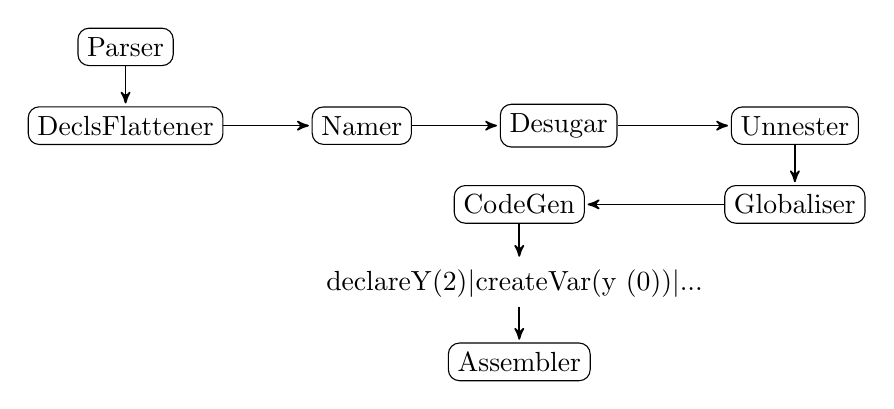
\begin{tikzpicture}[auto,every matrix/.style={ampersand replacement=\&,column sep=2cm,row sep=2cm},
                             to/.style={->,>=stealth',shorten >=1pt,semithick,font=\sffamily\footnotesize}]
  \node[pass](parser) at (0,1) {Parser};
  \node[pass](declsFlattener) at (0,0) {DeclsFlattener};
  \node[pass](namer) at (3,0) {Namer};
  \node[pass](desugar) at (5.5,0) {Desugar};
  \node[pass](unnester) at (8.5,0) {Unnester};
  \node[pass](globaliser) at (8.5,-1) {Globaliser};
  \node[pass](codegen) at (5,-1) {CodeGen};
  \node[txt](opcodes) at (5,-2) {\lstinline!declareY(2)|createVar(y(0))|...!};
  \node[pass](assembler) at (5,-3) {Assembler};

  \draw[to]  (parser.south) -- (declsFlattener.north);
  \draw[to]  (declsFlattener.east) -- (namer.west);
  \draw[to]  (namer.east) -- (desugar.west);
  \draw[to]  (desugar.east) -- (unnester.west);
  \draw[to]  (unnester.south) -- (globaliser.north);
  \draw[to]  (globaliser.west) -- (codegen.east);
  \draw[to]  (codegen.south) -- (opcodes.north);
  \draw[to]  (opcodes.south) -- (assembler.north);
\end{tikzpicture}
\caption{Compiler phases}
\label{fig:compiler_passes}
\end{figure}


These transformations are implemented by functions
taking as only argument the AST, and they return the transformed AST.
These functions all have the same structure, as displayed in Figure~\ref{fig:pass_structure}.
\begin{figure}[h]
\begin{lstlisting}
   fun {Transform AST}
      fun {TransformInt AST Params}
         case AST
         of ... then
         else
            {DefaultPass AST TransformInt Params}
         end
      end
      InitialParams = ...
   in
      {TransformInt AST InitialParams}
   end
\end{lstlisting}
\caption{Structure of a transformation function}
\label{fig:pass_structure}
\end{figure}
Having the same structure enables the use of the function
\lstinline!DefaultPass! listed in Figure~\ref{fig:default_pass}, which calls the
function passed as second arguments recursively on the AST with
\lstinline!Params! as last argument, but returns the root of the AST unchanged. This
facilitates the recursive calls for default behaviour on elements not modified
by the transformation.


\begin{figure}[h]
\begin{lstlisting}
   fun {DefaultPass AST F Params}
      % beware of the order. a record is also a list!
      if {List.is AST} then
         {List.map AST fun {$ I} {F I Params} end}
      elseif {Record.is AST} then
         case AST
         of pos(_ _ _ _ _ _) then
            % Do not go down into position records
            AST
         else
            {Record.map AST fun {$ I} {F I Params} end}
         end
      else
         AST
      end
   end
\end{lstlisting}
\caption{DefaultPass function}
\label{fig:default_pass}
\end{figure}



Params is a record with label \lstinline!params!, and features are added
as necessary. For example, this \lstinline!Params! argument is used by
the \lstinline!Globaliser! described in Section \ref{sec:arch:globaliser}. All
passes take a \lstinline!params! record as last argument, even if some do not use it. 
This early design decision proved very beneficial afterwards.
% Should I add that fAnd takes a pos feature and fAndThen not, and that I had to
% tweak the function WrapIn as a consequence?


Although all passes work exclusively on the AST, the transformations described in later sections can and will often be illustrated more clearly and concisely by giving the Oz code corresponding to the ASTs before and after the transformation. 

\subsection{Declarations Flattener}\label{sec:arch:declsflattener}
The Oz language accepts complex instructions in the declaration part of
\begin{lstlisting}
   local Decls in Body end
\end{lstlisting}
 It is thus necessary to identify the variables declared by each instruction present in the \lstinline!Decls!. 
For example, in unifications, only the left hand side variable gets declared,
and only \lstinline!B! is implicitly declared in the following code snippet:
\begin{lstlisting}
   local
      B=2*A
   in
      ...
   end
\end{lstlisting}
Fortunately, this has been clearly formalised by the Oz implementers and published on the web \cite{BaseLang}. This information has been included in Appendix \ref{appendix:patternvariables}. The namer simply applies these rules to move all code to the \lstinline!Body! beginning, keeping only simple variable declarations in \lstinline!Decls!.

\subsection{Namer}\label{sec:arch:namer}
The namer  basically replaces all occurrences of a variable's \lstinline!fVar! by \lstinline!fSym! tuples holding a symbol instance representing said variable. All uses of a variables are replaced by the same symbol instance. This symbol holds information about the variable, that will be completed by subsequent compiler passes, such as the type of the symbol, its allocated register,\ldots and is documented in Appendix \ref{appendix:symbol}.

In declarations, the namer creates a new symbol for the declared variables, in
other code, it looks at already defined symbols and replaces \lstinline!fVar!s
by a \lstinline!fSym! tuple containing the existing symbol for that variable.
This works because a variable can only be in the subtree whose root is the
variable declaration's instruction (be it a \lstinline!local Decls in Body end!
declaring variables in \lstinline!Decls!, a
\lstinline!proc {Id P1 P2}! declaring its formal parameters, \ldots) . The namer
can thus be sure to find a symbol for variables it encounters in the AST, or it
is an error.

The \lstinline!Namer! also has some work to do on patterns and the variables it
implicitly declares. As a consequence, it also handles and transforms the AST
for functions and procedures, which implicitly declare their formal parameters.

The set of maps from a variable name to its corresponding symbol is called environment, and is maintained by the namer.


\subsubsection{Declarations}
Variables can be declared in different ways and instructions.
One such instruction is of course the explicit declaration instruction
\lstinline!local Decls in Body end!, present in the AST in the form of
\lstinline!fLocal! tuples introduced in section \ref{sec:input:flocal}. At this
stage, \lstinline!Decls! only contains simple variables declaration, thanks to
the declaration flattener (see Section \ref{sec:arch:declsflattener}).
\lstinline!fLocal! introduces a new environment, in which the variables declared
in its first feature are added to the environment of the code present in its
second feature, possibly erasing mappings for variables with the same name
coming from the parent environment. 

It is these manipulations of the environments that make that the code in
Figure~\ref{fig:namer_nested_locals} does not throws an error of impossible
unification of A with 6. Indeed, the inner variable A gets another symbol
assigned than the outer one, and replaces it in the environment of the inner
instructions. Thus there is no ambiguity in the \lstinline!Show! instruction as
to which its argument is, and it effectively shows 6.

Another kind of declaration is found in the definition of procedures and
functions. Indeed, \lstinline!fProc! (Section~\ref{sec:input:procedures}) and
\lstinline!fFun! (Section~\ref{sec:input:functions}) tuples also implicitly
declare the variables for their formal parameters. % see test 029

Still another kind of declaration happens in pattern matching
(Section~\ref{sec:input:patternmatching}), when a record present in the pattern
has a feature that is a variable. This case is analysed specifically in
Section~\ref{sec:arch:namer:patternmatching}.

These variables get implicitly declared and added to the environment in which not only the clause' body but also its guards will be executed.


\begin{figure}
\begin{lstlisting}
local
   A=5
in
   local 
      A=6
   in
      {Show A}
   end
end
\end{lstlisting}
\caption{Nested locals handled by Namer}
\label{fig:namer_nested_locals}
\end{figure}


\subsubsection{Non-declaration code}
In code not declaring variables, the namer's transformation is much simpler: it will simply
replace all occurrences of \lstinline!fVar! tuples by a \lstinline!fSym! tuple having the corresponding symbol as first feature.


\subsubsection{Case Pattern Matching}\label{sec:arch:namer:patternmatching}
 Let's note
\lstinline!PatternX(Var1,Var2,..)! the Xth pattern tested and implicitly
declaring variables \lstinline!Var1!,\lstinline!Var2!,\ldots, and let's use the same convention for code fragments \lstinline!CodeX(Var1,Var2,..)! and guards \lstinline!GuardsX(Var1,Var2,..)! using those implicitly declared variables.

The transformation of the AST corresponding this Oz code:
\begin{lstlisting}
   case Val
   of Pattern1(A,B) andthen Guards1(A) then
      Code1(A,B)
   [] Pattern2(B,C) andthen Guards2(C) then
      Code2(B,C)
   else
      ElseCode
   end
\end{lstlisting}
results in an AST corresponding to this Oz code:
\begin{lstlisting}
   local
     A1 B1 B2 C2
   in
      case Val
      of Pattern1(A1,B1) andthen Guards1(A1) then
         Code1(A1,B1)
      [] Pattern2(B2,C2) andthen Guards2(C2) then
         Code2(B2,C2)
      else
         ElseCode
      end
   end
\end{lstlisting}

Here is the way how it is achieved. The compiler traverses each clause in turn,
and collects all symbols introduced during this operation. It creates a new
environment for this clause, which is updated with captures done in the
pattern. After that, the namer traverses the ASTs of the Guards and the Code
using this updated environment, and restores the original environment, on which
the next clause will build its own environment. This shows clearly that
although all capture variables are technically reachable from all clauses'
bodies, it will never be the case as the environment on which a clause builds
its own is the environment of the case instruction, not the environment updated
by the previous clause. 

In addition, the \lstinline!fSym! tuple corresponding to these capture
variables are themselves stored in an unforgeable secure structure (as
described in \cite{CTMCP} Section~3.7.5) which is itself wrapped in an
\lstinline!fConst!. The reason of this manipulation is to prevent manipulations
of those symbols by later compiler passes. Now these will be handled as
constants in all subsequent compiler passes. Another consequence of this is
that the records implicitly declaring variables in a pattern are seen as
constant records, all features being constants. And these are treated as such,
notably in the desugaring of records (section \ref{sec:arch:desugar:records}).

To ease the work of future passes and improve readability of their code, the
namer also replaces \lstinline!fEq! tuples of pattern conjunctions by
\lstinline!fPatMatConjunction! tuples.

Patterns with guards require some additional work. These are present in the AST
as 
\begin{lstlisting}
   fSideCondition(Pattern Decls Guards Pos)
\end{lstlisting}
First, a new symbol is
introduced and unified with the \lstinline!Guards! expression. The record in the
AST is replaced by 
\begin{lstlisting}
   fNamedSideCondition(Pattern Decls GuardsStatement GuardSymbol Pos)
\end{lstlisting}
where \lstinline!GuardStatement! is the unification of the newly
introduced symbol \\\lstinline!GuardSymbol!. The \lstinline!GuardSymbol! is
declared together with capture variables. 
This transformation cannot be completely represented in Oz code, notably the
transformation of the guards in statement. It will become clear when looking at
the \lstinline!CodeGen! why this transformation is done like this (the
description of the CodeGen code Section~\ref{sec:codegen:fNamedSideCondition} has more
details on page \pageref{sec:codegen:fNamedSideCondition}).


Escaped variables are transformed by the namer, which introduces a capture
symbol and then validates in a new guard that it has the value of the escaped variable.
 A pattern with an escaped variables, like \lstinline$rec(!Var)$ is
transformed in \lstinline!rev(Capt) and then Capt==Var!
Although this transformation might be seen as a \lstinline!Desugar! transformation, it is
done in the \lstinline!Namer! because it already traverses and transforms the
patterns, and all code infrastructure was already in place. Putting this
transformation in the \lstinline!Desugar! pass would have introduced code duplication.


\subsubsection{Pattern Arguments}
Functions and procedures in Oz can be defined with pattern arguments, which
destructures the argument and can shorten significantly the code:
\begin{lstlisting}
  fun {GetName person(name:Name ...)}
     Name
  end

  Name={GetName person(name:'Turing' firstname:'Alan')}}
\end{lstlisting}

The AST of this function's definition is actually transformed in an AST corresponding to the  code
listed in Figure~\ref{fig:getname2}.
\begin{figure}[h]
\begin{lstlisting}
  fun {GetName Arg }
     case Arg
     of person(name:Name ...) then
        Name
     end
  end
\end{lstlisting}
\caption{Pattern argument transformation result}
\label{fig:getname2}
\end{figure}


The namer thus replaces pattern variables by a synthetic symbol, and wraps the body of the function in case instructions (one level of case nesting for each pattern argument). 




\subsubsection{Classes}\label{sec:arch:namer:classes}
The work of the namer on classes is in most cases straight-forward. It goes through the tuple
\lstinline!fClass(Id Specs Methods Pos)! and names variables as one would expect:
method arguments are named as declarations i.e. it adds mappings to the
environment which are then used when traversing the body of the method.
It also goes through the attributes, features, properties and parents.

Difficulties arise though when methods have dynamic names, are private and/or
capture their head.

For method with a dynamic name, the namer simply has to use the binding for the
escaped variable in the current environment.

Private methods have their label defined as a variable. The namer will transform this by 
declaring a new symbol for the variable and bind it to a new name.
The transformation can be illustrated in Oz code, transforming

\begin{lstlisting}
   class C
      meth init skip end
      meth A()
         Body
      end
   end
\end{lstlisting}

in

\begin{lstlisting}
  local
     A
   in
      A={NewName}
      class C
         meth init skip end
         meth !A()
            Body
         end
      end
\end{lstlisting}

Note also that the variable being the label of the method can have the same name
as the class. Inside the class the variable will reference the method, and not the class, 
as illustrated in Figure~\ref{fig:class_method_binding}. The private methods'
variables are available inside the class, overriding the mapping to the class
\lstinline!C!.
\begin{figure}[h]
\begin{lstlisting}
   class C
      meth init skip end
      meth C(M)
         {Show M}
      end
      meth whisper(M)
         {self C(M)}
      end
   end
\end{lstlisting}
\caption{Private method overriding the mapping of C}
\label{fig:class_method_binding}
\end{figure}



We can now look at the situation when the method head is captured (see
Section~\ref{compilerinput:classes:headcapture} page
\pageref{compilerinput:classes:headcapture} for the AST form).
Figure~\ref{fig:attentionpoints} lists code illustrating the specific points requiring attention.
\begin{figure}[h]
\begin{lstlisting}
   class C
      meth init skip end
      meth echo(F ...)=C
         {Show C}
      end
      meth whisper(F ...)=C
         {Show F}
      end
      meth clone()
        {New C init}
      end
   end
\end{lstlisting}
\caption{Class definition}
\label{fig:attentionpoints}
\end{figure}

These attention points are:
\begin{itemize}
  \item the same variable name can be used by multiple methods to store their
    respective method heads
  \item the variable holding the method head has to be available only to the
    method defining it
  \item the variable can have the same name as the class in which the method is
    defined (\lstinline!C! in method \lstinline!clone! references the class \lstinline!C!)
\end{itemize}

Again, when the namer enters a method, it defines a new environment.

Having covered all special behaviour to support, we can now look at how the namer works to 
respect these constraints.

We have seen that the namer has to be able to declare and initialise new
variables which will be available inside the class only. As a consequence, the
namer will maintain a list of symbols to be declared with their respective
initialisation code.

The namer starts by naming the class.

It then creates a new environment, and names all method labels (and only the
labels, not the arguments, not the variable capturing the method head).
Variables named in this step will be available to all methods of the class.
They correspond to labels of private methods, and their initialisation code is
simply unifying them with a new name.

It will then go through all methods again to name their respective arguments,
body and possible method head capture variable. For each method it will take
these actions in order
\begin{enumerate}
  \item create new environment
  \item name the method head capture variable as declaration if it was defined
  \item name the method's arguments as declaration
  \item name the body
  \item restore the previous environment
\end{enumerate}

It then wraps the class definition in a \lstinline!local..in..end! declaring the
variables to be declared collected while traversing the class (these are
variables that were encountered as method label), and prepend the class
definition by the initialisation code collected:


\subsubsection{Exceptions}\label{sec:arch:namer:exceptions}
The AST received by the namer for a try instruction is:
\begin{lstlisting}
   fTry(
      Body
      fCatch(
         |(
            fCaseClause(
               Pat1
               Code1)
            |(
               fCaseClause(
                  Pat2
                  Code2)
               nil))
         pos)
      FinalCode
      pos)
\end{lstlisting}

The namer will traverse \lstinline!Code! and \lstinline!Finally! and name variables based on existing
mappings present in the environment. The patterns of a catch clause is
handled exactly (in the sense that it is the same compiler code that is called)
as the pattern of a case clause (see Section \ref{sec:arch:namer:patternmatching}).
A new environment is created for each clause, to which the pattern might add
bindings, which are then available when naming the code of the clause.
New symbols are possibly introduced by the patterns, which then have to be
declared in a \lstinline!local..in..end! instruction wrapping the named
\lstinline!try!  instruction. This construction is very similar to the one
presented in Section~\ref{sec:arch:namer:patternmatching}.

\subsubsection{Functors}\label{sec:arch:namer:functors}
The work done by the namer on \lstinline!fFunctor(Id SpecsList Pos)! nodes is trivial, but the
order of naming the items of the \lstinline!SpecsList! is important. For
example, \lstinline!import!ed variables have to be named before traversing the
\lstinline!define! block, or else these wouldn't be available to that code!

It is possible to sketch the scope of variables introduced by a functor with the code in
Figure~\ref{fig:functors_scope}. The variables declared by \lstinline!require!
are available to all other parts of the functor, which is not the case of the
variables defined by \lstinline!prepare!, which are not available in the
\lstinline!require! statements. 

\begin{figure}[ht]
\begin{lstlisting}
   local
      require_decls
   in
      require_stats
      local
         prepare_decls
      in
         prepare_stats
         local
            import_decls
         in
            import_stats
            local
               define_decls
            in
               define_stats
               exports
            end
         end
      end
   end
\end{lstlisting}
\caption{Functor variables scopes}
\label{fig:functors_scope}
\end{figure}

One other small change introduced by the namer is the creation of default export
key, changing
\begin{lstlisting}
   export
      DumpAST
\end{lstlisting}
in
\begin{lstlisting}
   export
      dumpAst:DumpAST
\end{lstlisting}

\nav{The next transformation applied on \lstinline!fFunctor! nodes is found in
the desugar pass, Section~\ref{sec:arch:desugar:functors}.}



\subsubsection{For loops}
Loops over a list are transformed in a call to \lstinline!ForAll! which is then
recursively named. Note that the behaviour of a for loop over multiple lists is not correct with this implementation and
as a consequence the test number 133 of the test suite does not currently pass. The correction of this code is mentioned in the ``Future work'' section on page \pageref{sec:futurework}.

Loops over an integer range are first transformed in a call
to \lstinline!for! and then recursively named.

C-like loops are currently not supported.

\subsubsection{Compiler Code Notes}
The namer is one function unimaginatively named \lstinline!Namer! taking as argument an AST, and returning the resulting AST.
The following local functions are defined: \lstinline!NamerForDecls!,\lstinline!NamerForBody!,\lstinline!NamerForCaptures!.
Notice that \lstinline!NamerForBody! calls \lstinline!NamerForDecls! when a function or procedure is
defined, and calls \lstinline!NamerForCaptures! for patterns in \lstinline!fCaseClause!s. 
Figure~\ref{fig:namer:ffun} lists the code handling a definition in non-declaration part of a
function with no pattern argument:

\begin{figure}[h]
\begin{lstlisting}
  %---------------------------------
  [] fFun(Name Args Body Flags Pos) then
  %---------------------------------
     Res
  in
     {Params.env backup()} 
     Res=fFun(
        % The function's variable has to be declared explicitely 
        % in the declaration part.
        % That's why we call NamerForBody on the Name
        {NamerForBody Name Params}
        % Formal parameters are declarations, that's why we 
        % call NameForDecls
        {List.map Args fun {$ I} {NamerForDecls I Params} end }
        {NamerForBody Body Params}
        Flags
        Pos
     )
     {Params.env restore()}
     Res
\end{lstlisting}
\caption{Namer transformation of fFun nodes}
\label{fig:namer:ffun}
\end{figure}


The environment, mapping variable names to their respective symbol, is stored in
the object available through \lstinline!Params.env!. This object's
\lstinline!backup! method will backup the current environment and create a new
one with the exact same bindings.
The function creates a new environment based on its parent environment, which is
backed up to be restored when done. The name of the function is passed to \lstinline!NamerForBody!, because the name of the function must have been declared previously and be present in the environment. 
The formal parameters of the function however are passed to \lstinline!NamerForDecls!, as these are variables implicitly declared, that have to be added to the current environment. This updated environment is then used by \lstinline!NamerForBody! to transform the function's body.
At the end, the parent's environment is restored, ensuring that formal parameters of the function are not available outside of the function.

This code also illustrates how functions can access variables
available in the defining environment (such functions are called closures): all
those are inherited by the function's environment.

Some parts of the namer code are not that simple. For example \lstinline!NamerForBody! 
declares a function \lstinline!HandlePatternArgs!
to apply the described transformation of functions and procedures with patterns
arguments. 

Handling \lstinline!fCase! nodes also requires more work as it needs to 
\nopagebreak[4]
\begin{itemize}
  \item declare new capture variables
  \item handle guards by, amongst other things, introducing a new symbol
  \item add guards corresponding to escaped variables in patterns
\end{itemize}
The function \lstinline!NamerForCaptures! is called on the case patterns, collecting symbols
to be declared in \lstinline!Params.captures!.
New symbols introduced for escaped variables are collected in
\lstinline!Params.guardsSymbols!. 

As for the work of the namer in case of classes, it involves several steps as described
in Section \ref{sec:arch:namer:classes}.
Several functions are defined to help these steps. \lstinline!NameMethodLabel!
is the function used when traversing the methods list the first time to name
only the method labels.
\lstinline!NameMethod! is used when traversing the methods the second time to
name the arguments and the body.

Once these functions are defined, the namer's code for classes is quite simple,
and listed in Appendix~\ref{appendix:classnamer} to illustrate the different steps.


The code traversing \lstinline!catch! patterns makes use of the same
function used for naming \lstinline!case! clauses, namely
\lstinline!NamerForCaptures!.



\subsection{Desugar}\label{sec:arch:desugar}
The desugar pass handles the transformation of syntactic sugar code in its canonical form.
Oz distinguishes two groups of instructions: statements and expressions. An expression is ``syntactic sugar for a sequence of operations that return a value'' \cite{CTMCP}. Statements do not return a value.
The desugar function handles statements and expression differently, and defines two local functions, one for handling expressions, one for handling statements.
\subsubsection{On statements and expressions}
Handling expressions and statements is often very similar, but sometimes require significant differences of treatment. Hence the use two different local functions in the Desugar pass.

It is important that a lot of instructions can be used both as expression and as
statement. Here is an example.
In Oz, a cell is a mutable storage element which is created with an initial value (\lstinline!C={NewCell 0}!), it can be given a new value (\lstinline!C:=NewValue!) and its value can be read (\lstinline!@C!). There's also an exchange operation \lstinline!{Exchange C Old New}! which ``atomically binds Old with the old content of the cell, and set New to be the new content'' \cite{CTMCP}.%page 415.
Assigning a new value to a cell is usually a statement returning no value, but
when used as the right hand side of an unification, it becomes an expression,
whose value is the Old value of the cell.
\begin{figure}[h]
\begin{lstlisting}
local
  C={NewCell 0}
  Old
in
  C:=1        % statement
  Old=(C:=2)  % expression, whose value is assigned to Old
  {Show Old}  % displays 1
end

\end{lstlisting}
\caption{Cell assignment as statement and as expression}
\label{fig:statement_and_expression1}
\end{figure}

Determining if an instruction is a statement or and expression is done
recursively from top to bottom, the starting case being that the program is a
statement. In Figure \ref{fig:statement_and_expression1}, the
whole code snippet which we consider in this case as a complete program is a
statement. This \lstinline!local...in...end! instruction is thus a statement.
The declaration part of this instruction is always a list of \lstinline!fSym!. The body is
also a statement because the whole \lstinline!local...in...end! is a statement. If it were
an expression, the body
would have been an expression. In our case, the body is a sequence of
instructions, resulting in a hierarchy of \lstinline!fAnd! tuples in the AST. Thus we see that a sequence
can be a statement or an expression, in the latter case the value
of the whole sequence is the value of the last instruction which must be an expression. This illustrates the
need of distinct functions when statement and expressions must be handled
differently. 

If we note \lstinline!F! the pass of the compiler, \lstinline!FExpr! the locally defined
function handling expressions, and \lstinline!FStat! corresponding function for
statements, we can ensure that the right function is applied to each
instruction's AST as defined in section \ref{section:compilerinput} by following
these rules of identification, and call \lstinline!FStat! on statements and
\lstinline!FExpr! on expressions:

\begin{description}
  \item[program] the program is a statement
  \item[fLocal] 
    \begin{itemize}
      \item the declarations are all just \lstinline!fSym!s, since the
        \lstinline!DeclsFlattener! has
        moved all other code to the body. These \lstinline!fSym!s are neither
        expressions nor statements, they are just \lstinline!fSym! declarations
      \item the body is of the same kind as its parent \lstinline!fLocal!
    \end{itemize}
  \item[fAnd] 
    \begin{itemize}
      \item the first feature is a statement
      \item the second feature is of the same kind as its parent \lstinline!fAnd!
    \end{itemize}
  \item[fEq] both sides are expressions
  \item[fProc] if the procedure's definition is an expression, its identifier
    must be the nesting marker \$, else its identifier is an expression. The
    arguments are patterns, and the body is a statement except if one of its
    formal parameters has a nesting marker, in which case the body is an
    expression.
  \item[fFun] are similar to \lstinline!fProc!, because a function definition is desugared
    in a procedure definition as described in Section
    \ref{sec:arch:desugar:functions}. The body of a \lstinline!fFun! is an expression.
  \item[fApply] calls can be statements or expressions, but in both cases the callee and its arguments are all expressions. 
  \item[fColonEquals] can be statement or expression, but \lstinline!Cell! and
    \lstinline!Val! are in both cases expressions.
  \item[fAt(Cell Pos)] can only be used as an expression. \lstinline!Cell! is an expression.
  \item[fRecord] can only be used as expressions. Its label, features and values are
    expressions.
  \item[fCase] can be a statement or an expression. The value tested is an
    expression. The \lstinline!fCaseClause!s
    and the else code have the same type as their parent \lstinline!fCase!. The patterns in
    the \lstinline!fCaseClause!s are patterns, and the guards are expressions.
\end{description}

All expressions and statements in the AST will be visited by Desugar. Even if the statement itself is not transformed, as is the case for a unification, its children will be visited and possibly transformed. For example
\lstinline!X=5+2! will still be a unification after it's been desugared, but its
children will have been transformed in \lstinline!X={Number.'+' 5 2}!.



\subsubsection{Operators}
Operators are transformed in the call of their respective function as listed in Table~\ref{table:operators}.

\begin{table}[h]
\begin{center}
\begin{tabular}{| l l |}
  \hline
  Operator & Desugar result \\
  \hline
  \lstinline!+! & \lstinline!Number.'+'! \\
  \lstinline!*! & \lstinline!Number.'*'! \\
  \lstinline!-! & \lstinline!Number.'-'! \\
  \lstinline!~! & \lstinline!Number.'~'! \\
  \lstinline!div! & \lstinline!Int.'div'! \\
  \lstinline!mod! & \lstinline!Int.'mod'! \\
  \lstinline!/! & \lstinline!Float.'/'! \\
  \lstinline!==! & \lstinline!Value.'=='! \\
  \lstinline!>=! & \lstinline!Value.'>='! \\
  \lstinline!=<! & \lstinline!Value.'=<'! \\
  \lstinline!>! & \lstinline!Value.'>'! \\
  \lstinline!<! & \lstinline!Value.'<'! \\
  \lstinline!\\=! & \lstinline!Value.'\\='! \\
  \lstinline!:=! & \lstinline!Value.catExchange! \\
  \hline
\end{tabular}
\end{center}
\caption{Operators and their desugar result}
\label{table:operators}
\end{table}



The operators are parsed as \lstinline!fOpApply! tuples as described in section \ref{sec:input:operators}. Building further on the example of that section, the AST coming from the parser

\begin{verbatim}
      fOpApply(
         '+'
         [ fInt(5 pos)
           fInt(2 pos) ]
         pos)
\end{verbatim}
will be transformed in:
\begin{verbatim}
      fApply(
         Number.'+'
         [ fInt(5 pos)
           fInt(2 pos) ]
         pos
      )
\end{verbatim}

\subsubsection{Functions}\label{sec:arch:desugar:functions}
Functions are transformed in their canonical procedure form. This is done simply by replacing the function by a procedure with exactly the same characteristics, except that it takes one additional argument (the return value), and the body of this procedure is the unification of this new argument with the original body of the function. This resulting AST is itself recursively desugared.

For example, the code
\begin{lstlisting}
   fun {F A B}
      A+B
   end

\end{lstlisting} 
will have its AST transformed such that it corresponds to this Oz code:
\begin{lstlisting}
   proc {F A B ?R}
      R={Number.'+' A B}
   end
\end{lstlisting} 
A new symbol, denoted \lstinline!R! for convenience, is added to the arguments list of the procedure, and this new symbol is then unified with the body of the original function. This unification will in turn be handled by the unnester, which is the next pass of the compiler.


The function definition is parsed in the AST of Figure~\ref{fig:fundef} 
and transformed by the desugar pass into the AST in Figure~\ref{fig:fundesugar}.
\begin{figure}[h]
\begin{verbatim}
      fFun(
         fSym(F pos)
         [  fSym(A pos)
            fSym(B pos) ]
         fOpApply(
            '+'
            [ fSym(A pos)
              fSym(B pos)]
            pos)
         pos)
\end{verbatim}
\caption{Function definition}
\label{fig:fundef}
\begin{verbatim}
     fProc(     
         fSym(F)
         [  fSym(A pos)
            fSym(B pos)
            fSym(R pos) ]
         fEq(
            fSym(R)
            fApply(
               fConst('+' pos)
               [  fSym(A pos)
                  fSym(B pos)]
               pos)
            pos)
         pos)
\end{verbatim}
\caption{Desugared function definition}
\label{fig:fundesugar}
\end{figure}



Lazy functions have in their flags a lazy atom: \lstinline!fAtom(lazy pos)!.
The desugar step of lazy function consists in wrapping in a thread a call to the builtin \lstinline!waitNeeded! on the return symbol before unifying it with the body of the function. If the function of the previous example had been marked as lazy, the transformation would have yielded this result, in Oz notation:
\begin{lstlisting}
   proc {F A B ?R}
      thread 
         {WaitNeeded R}
         R={Number.'+' A B}
      end
   end
\end{lstlisting} 

\subsubsection{Procedures}\label{sec:arch:desugar:procedures}
The only special operation in desugaring procedure definitions, is the case
 procedures having the nesting marker as one of
their formal parameters. At the call, the argument passed in place of the
nesting marker will be unified with the body of the procedure which much be an
expression. 
Understanding this makes the transformation immediate. For example, this procedure
\begin{lstlisting}
      proc {Succ In $}
         In+1
      end
\end{lstlisting}

will be desugared in

\begin{lstlisting}
      proc {Succ In R}
         R=In+1
      end
\end{lstlisting}
\subsubsection{Calls}\label{sec:arch:desugar:calls}
A node \lstinline!fApply(Op Args Pos)! has \lstinline!Op! and \lstinline!Args!
desugared as expressions.
\nav{The next operation on an fApply node takes place in the unnester, see Section
\ref{sec:arch:unnester:calls}.}
\subsubsection{Records}\label{sec:arch:desugar:records}
As mentioned in the description of records in Section \ref{sec:input:records},
the features can be left out, and are in that case implicit, with increasing
integer values starting from 1. The Desugar pass will make these features explicit.

In Oz syntax, it means that \lstinline!rec(a b c)! is transformed in
\lstinline!rec(1:a 2:b 3:c)!. Of course, attention has to be paid by the
programmer to avoid conflict, as implicit feature assignment does not check for
explicit features'values, and conflict can arise. For example \lstinline!rec(a 1:b c)! will be transformed in \lstinline!rec(1:a 1:b 2:c)!. This behaviour is
consistent with Mozart 1.

Records undergo two additional transformations. First, \lstinline!fRecord! that
have all label, features and values constant are replaced by a
\lstinline!fConst! with as value the record reconstructed. This greatly
simplifies the AST for these records as is illustrated in the next example, and
can be done because the value of the record can be used as is in later steps,
notably the opcodes generation. This transformation is called constant folding.
\begin{lstlisting}
      fRecord(
         fAtom(rec pos)
         [
            fColon(
               fInt(1 pos)
               fAtom(a pos)
            )
            fColon(
               fInt(2 pos)
               fAtom(b pos)
            )
         ]
      )
\end{lstlisting}
is transformed in
\begin{lstlisting}
  fConst( rec(1:a 2:b) pos)
\end{lstlisting}


Records with non constant labels and/or features are replaced by a call to
\lstinline!Boot_Record.makeDynamic!, \lstinline!Boot_Record! being a builtin module (a module implemented in C++ and made available to the Oz code as if it was a functor). The goal of this transformation is to leave
in the AST only records with constant label and features.
\lstinline!MakeDynamic! takes two arguments. First the label of the record to construct. And second, a tuple with label '\#' and whose values are alternately the features and their respective value. As a result, we replace \lstinline!Rec(F1:V1 F2:V2)! by 
\begin{lstlisting}
   {Boot_Record.makeDynamic Rec '#'(1:F1 2:V1 3:F2 4:V2)}
\end{lstlisting}

We end up with an AST that only contains records with constant label and features: only the values are not constants.
This is required because there is no opcode capable of handling a record with non-constant arity.

\subsubsection{Pattern Matching}
Records and open records present in a pattern undergo the same desugar
transformation as normal records. Patterns however can only have constant label
and features.
\subsubsection{Wildcards}
Although the programmer is not interested in these values, the compiler will declare and place a new synthetic symbol in each of these locations. In oz code notation, \lstinline!_! is replaced by the expression \lstinline!local NewSymbol in NewSymbol end!.
Patterns with guards, found in the AST as 
\begin{lstlisting}
   fNamedSideCondition(Pattern Decls Guards GuardSymbol Pos)
\end{lstlisting}
have their features handled according their statement/expression character:
\lstinline!Pattern! is a pattern, \lstinline!Decls! are left as is,
\lstinline!Guards! is a statement (see the introduction
of \lstinline!fNamedSideCondition! by the namer in Section
\ref{sec:arch:namer:patternmatching}) and \lstinline!GuardSymbol! is just a
symbol, left as is.

Pattern conjunctions, present in \lstinline!fPatMatConjunction! records, have
their features desugared and are then placed in a secure structure like
\lstinline!fSym! in
patterns are by the namer (Section \ref{sec:arch:namer:patternmatching}).
This is done because no other transformation should be done on the pattern
conjunction's member before it is used by the code generator.


\subsubsection{Threads}
A thread expression \lstinline!thread Body end! is desugared in the resulting
statement 
\begin{lstlisting}
   local 
      X 
   in 
      thread X=Body end 
      X 
   end 
\end{lstlisting}

This statement is then itself desugared.

Transforming a thread statement consists in the creation of a procedure with no
argument whose body is the desugared body (which is a statement) of the thread,
and then passing this procedure to the internal \lstinline!Thread.create!
procedure.
In Oz notation, \lstinline!thread Body end! is transformed in 
\begin{lstlisting}
   local 
      P 
   in 
      proc {P} 
         DesugaredBody 
      end 
      {Thread.create P}
   end
\end{lstlisting}
At the AST level \lstinline!fThread(Body Pos)! is transformed in this AST (taken from the compiler source code):
\begin{lstlisting}
  fLocal(NewProcSym 
         fAnd( fProc(NewProcSym nil {DesugarStat Body Params} nil pos) 
               fApply(fConst(Boot_Thread.create pos) [NewProcSym] pos)
             ) 
         Pos)
\end{lstlisting}

\subsubsection{Locks}
Locks statements are handled very similarly to thread statements: their body is
wrapped in a argumentless procedure, which is passed as argument, together with
the lock itself, to the base environment's \lstinline!LockIn!. In Oz notation, \lstinline!lock L then Body end! is transformed in
\begin{lstlisting}
local
   P
in
   proc{P}
      Body
   end
   {LockIn L P}
end
\end{lstlisting}


\subsubsection{If then else}
The condition tested is always an expression.
The instruction itself can be a statement as in 
\begin{lstlisting}
   if Cond then {DoTrue} else {DoFalse} end
\end{lstlisting}
in which case both code branches are desugared as statement
or an expression as in
\begin{lstlisting}
   X=if Y>Z then bigger else smallerOrEqual end
\end{lstlisting}
in which case both code branches are desugared as expression.
A \lstinline!fNoElse! tuple is left as is and will only be useful for the opcode generation function.

\subsubsection{Case}
The case instruction is very similar to \lstinline!if..then..else..end!.
The condition tested is always an expression.
The \lstinline!case! instruction can be a statement as in Figure~\ref{fig:casestat}
, in which case clauses are desugared as statement or an expression as in Figure~\ref{fig:caseexpr}
in which case each clause is desugared as an expression.
\begin{figure}[h]
\begin{lstlisting}
   case Rec
   of action(A) then
      {DoAction A}
   [] 'skip'() then
      skip
   [] else
      {LogError}
   end
\end{lstlisting}
\caption{Case statement}
\label{fig:casestat}
\end{figure}

\begin{figure}[h]
\begin{lstlisting}
   PersonId= case Rec
             of create(Name) then
                Person = {Create Name}
             in
                Person.id
             [] find(Name) then
                Person = {Find Name}
             in
                if Person==unit then
                   unit
                else
                   Person.id
                end
             [] else
                unit
             end
\end{lstlisting}
\caption{Case expression}
\label{fig:caseexpr}
\end{figure}

\pagebreak[4]
As for the \lstinline!if..then..else! instruction, the absence of an else clause
is indicated by a tuple \lstinline!fNoElse! in the AST. If no else clause was
present, the desugar step introduces one which raises an error, transforming

\nopagebreak[4]
\begin{lstlisting}
   case Rec
   of action(A) then
      {DoAction A}
   end
\end{lstlisting}
in
\begin{lstlisting}
   case Rec
   of action(A) then
      {DoAction A}
   else
      {Boot_Exception.'raiseError' kernel(noElse File Line Rec)}
   end
\end{lstlisting}

\subsubsection{Booleans Combinations}
Conjunctions of boolean expressions with \lstinline!andthen! are desugared in
\lstinline!if..then..else! expressions. Here is the translation
rule:
\lstinline!Cond1 andthen Cond2! is translated in \lstinline!if Cond1 then Cond2 else false end! 
We see that conditions are evaluated from left to right, and that conditions
evaluation stops as soon as possible, i.e. when a false condition is
encountered.

\lstinline!orelse! combinations are similarly translated from \lstinline!Cond1 orelse Cond2! to \lstinline!if Cond1 then true else Cond2 end!  
The example of Figure~\ref{fig:desugar:orelsesrc} is transformed in the code in
Figure~\ref{fig:desugar:orelse}.
\begin{figure}[h]
\begin{lstlisting}
(A==1 andthen B==2) orelse C==3
\end{lstlisting}
\caption{\lstinline!orelse! code to be desugared}
\label{fig:desugar:orelsesrc}
\end{figure}

becomes

\begin{figure}[h]
\begin{lstlisting}
if (if A==1 then B==2 else false end)
then
  true
else
  C==3
end
\end{lstlisting}
\caption{Desugaring \lstinline!orelse!}
\label{fig:desugar:orelse}
\end{figure}


This form will then be handled by later passes of the compiler.
\subsubsection{Classes}\label{sec:arch:desugar:classes}
Handling classes in the
compiler consists in desugaring the class definition in a call to
\lstinline!OoExtensions.'class'!. 
The AST node \lstinline!fClass(FSym Specs Methods Pos)! gets transformed in 
\begin{lstlisting}
   fApply(fConst(OoExtensions.'class' Pos) 
          [Parents Meths Attrs Feats Props PrintName FSym] 
          Pos)
\end{lstlisting}

The \lstinline!Desugar! function just has to correctly build the arguments of
the call. Of course, the arguments are themselves ASTs. So an argument that is a
list will be in fact an \lstinline!fRecord!.

Information to build the elements \lstinline!Parents!, \lstinline!Attrs!,
\lstinline!Feats! and \lstinline!Props! come from the \lstinline!Specs! value in
the \lstinline!fClass! node.

\lstinline!Parents! is simply a list of the parents of the class. The elements
of the list are simply the \lstinline!fSym! tuple holding the symbols
corresponding identifying the parent classes.


\lstinline!Meths! is a \#-tuple with one item of the form \lstinline!name#Proc! for each
method, where \lstinline!name! is the method name, and Proc is a procedure
(which we will characterise as a ``proxy'' procedure) with
2 arguments implementing the method. The two arguments of the method are
\lstinline!self!,
which is the object on which the method is called, and \lstinline!M!, the message
corresponding to the call. It is the message that contains all argument values.
It is important to note that the symbols used inside the body of the method
don't correspond to the arguments of the procedure implementing the method.
This mismatch is handled by unifying symbols in the method body with values
found in the message. Figure~\ref{fig:methimpl} shows a methods and its implementing procedure.
\begin{figure}[h]
\begin{lstlisting}
  meth foo(X Y)
     {Show X+Y}
  end 
\end{lstlisting}
\caption{Example method}
\begin{lstlisting}
  proc {Foo Self M}
     X Y
  in
     X = M.1
     Y = M.2
     {Show X+Y}
  end  
\end{lstlisting}
\caption{Procedure implementing example method}
\label{fig:methimpl}
\end{figure}

Of course, the compiler handles keyed arguments, where the features of the
message \lstinline!M! are not only numeric.

As described in Section~\ref{compilerinput:classes:headcapture} on page \pageref{compilerinput:classes:headcapture}, the message
corresponding to the method call can be captured and made available to the body of the
method. The message being the second argument of the ``proxy'' procedure, it is
easy to make it available in the method body by prepending it with a unification
of the header capture symbol and the message symbol itself. A better approach
might be to use the capture symbol directly as the message symbol in a future
revision of the code.

Handling default values needs special care. The unification of the symbol with its default value may only be done
if no value was provided in the message \lstinline!M!. But this can only be done at run time, hence the compiler
has to inject code in the AST to check if a value was provided for the method argument.
Here is the code injected in the AST, where \lstinline!Index! is the index of the argument that is handled and 
\lstinline!MessageSymbol! is the symbol corresponding to the message of the method
call:
\begin{lstlisting}
      fEq(Sym 
          fBoolCase(fApply(fConst(Value.hasFeature pos) 
                           [MessageSymbol fConst(Index pos)] pos)
                    fOpApply('.' [MessageSymbol fConst(Index pos) ] pos)
                    Default 
                    pos) 
          pos)
\end{lstlisting}
which, written in Oz, is:
\begin{lstlisting}
  Sym=if {Value.hasFeature MessageSymbol Index} then 
         MessageSymbol.Index 
      else
         Default
      end
\end{lstlisting}

Note that this code behaviour is different from 
\begin{lstlisting}
   {CondSelect MessageSymbol Index Default}
\end{lstlisting}
as in the latter case, all arguments of \lstinline!CondSelect! will be evaluated
first. 

The body of the method is desugared with an additional bit of information compared to normal procedures: the symbol corresponding to \lstinline!self!, the object on which the method is called. 
The availability of \lstinline!self! is not the only difference in the desugarisation of the methods' bodies. Some operators also have another meaning inside methods, like for example \lstinline!@!.
In code outside methods, \lstinline!@! is desugared in a call to
\lstinline!Boot_Value.catAccess!, but in methods, it has to be desugared in a
call to \lstinline!Boot_Value.catAccessOO!. There is a similar change for other
operators like \lstinline!:=! and the exchange operation.
Some operators are only available in methods, such as the attribute assignation
operator \lstinline!<-!. It is desugared in 
\lstinline!{BootObject.attrAssign Self LHS RHS}!.

Just as procedures, methods can have the nesting marker as formal parameter. The transformation needed
is exactly the same as explained in Section \ref{sec:arch:desugar:procedures} for functional procedures.

\lstinline!Attrs! is a record with label \lstinline!attr!.
For each attribute of the class, there is a feature-value pair in that record.
The feature is the name of the attribute, the value is the default value
provided in the class definition, or the result to a call to
\lstinline!{Boot_Name.newUnique 'ooFreeFlag'}!

\lstinline!Feats! is a record with label \lstinline!feat! built exactly in the
same way as \lstinline!Attrs!, but with the features present in the class
definition.

\lstinline!Props! is similar to \lstinline!Parents! in that it is simply a list of properties of the class (\lstinline!final!,
\lstinline!locking!). The \lstinline!locking! property implicitly declares a
lock object for the class, which can then be used with the \lstinline!lock!
instruction, which then appears in the AST as \lstinline!fLock(Body Pos)!, which
differs from the nodes \lstinline!fLockThen! described in Section
\ref{sec:input:locks}, notably because it doesn't take the lock object as
argument. \lstinline!fLock!
needs to be desugared to make the lock object explicit. Instance an instance of
a class, the lock object can be obtained by a call to
\lstinline!OoExtensions.'getObjLock'!, which can then be used in a
\lstinline!fThenLock! instruction. In practice, the node
\label{desugar:classes:lock}
\begin{lstlisting}
   fLock(Body Pos)
\end{lstlisting}

will be desugared in 

\begin{lstlisting}
   fLockThen( fApply(fConst(OoExtensions.'getObjLock' Pos) 
                     [@(Params.'self')] 
                     Pos)
              Body 
              Pos)  
\end{lstlisting}
which is itself desugared.

\lstinline!PrintName! is an atom which is the name of the class, or \lstinline!''! if it is
an anonymous class.

This is all the compiler has to do to support classes. From this point, the AST
has no more references to classes. The virtual machine will handle everything related to classes for us.

\subsubsection{Exceptions}\label{sec:arch:desugar:exceptions}
\lstinline!fRaise! nodes are desugared in a call to the builtin
\lstinline!Exception.'raise'!. The exception is an expression, and desugared as
such, transforming
\begin{lstlisting}
   fRaise(E pos)
\end{lstlisting}
in
\begin{lstlisting}
   fApply(
          fConst(Exception.'raise' pos) 
          [ {DesugarExpr E Params} ] 
          pos)
\end{lstlisting}
\pagebreak[4]
As a reminder, here is the AST of a try instruction:
\nopagebreak[4]
\begin{lstlisting}
   fTry(
      Body
      fCatch(
         |(
            fCaseClause(
               Pat1
               Code1)
            |(
               fCaseClause(
                  Pat2
                  Code2)
               nil))
         pos)
      FinalCode
      pos)
\end{lstlisting}
Desugaring an \lstinline!fTry! node without \lstinline!finally! code is not much
more complex.  If the try instruction is an expression (resp. statement), the
body and the clauses' code are desugared as expressions (resp. statements).
A \lstinline!case! instruction is introduced, using the very same clauses as the
catch, transforming \cite{BaseLang}
\begin{lstlisting}
  try SE1 
  catch C1 [] ... [] Cn 
  [[ finally S ]]
end
\end{lstlisting}

in

\begin{lstlisting}
try SE1 
catch X then 
   case X of C1 [] ... [] Cn 
   else 
      raise X end 
   end 
[[ finally S ]]
end
\end{lstlisting}

As this code shows, the very same clauses can be reused for the case
instruction, without the need of complex AST transformation.

Note that an \lstinline!else! clause is introduced in the \lstinline!case!
instruction. This is simply to re-raise the exception if no pattern matched,
meaning that the exception was not caught at this level.
In the transformed code, note also that a new symbol, \lstinline!X! is
introduced. 
\pagebreak[4]
This results in the new AST transformation for a try expression from
\begin{lstlisting}
   fTry(Body fCatch(Clauses CatchPos) fNoFinally Pos)
\end{lstlisting}
to
\begin{lstlisting}
  fLocal(  NewSymbol
           fTry({DesugarExpr Body Params} 
                fCatch([fCaseClause(NewSymbol 
                                    {DesugarExpr fCase(NewSymbol 
                                                       Clauses 
                                                       fRaise(NewSymbol Pos) 
                                                       CatchPos) 
                                                 Params})] 
                       CatchPos) 
                fNoFinally 
                Pos)
           Pos)
\end{lstlisting}

Desugaring an \lstinline!fTry! node with a \lstinline!finally! block is more
involved, and although the logic is similar, handling try-finally expressions and
statements requires some differences of treatment.

The transformation arises from the fact that the \lstinline!finally! code has to
be executed, even when an exception was raised.
Let's examine the transformation of \lstinline!try! statements, which
transforms this

\begin{lstlisting}
  try Body
  finally S 
  end
\end{lstlisting}

to

\begin{lstlisting}
  local X in 
     X = try 
            try Body end 
            unit 
         catch Y then ex(Y)
         end 
     S 
     case X of ex(Z) then 
        raise Z end 
     else skip 
     end 
end  
\end{lstlisting}

This example does not include \lstinline!catch! clauses for brevity. They can be considered
as being part of \lstinline!Body!.
A new variable (\lstinline!X!) is introduced and unified with a new try
expression whose body is a sequence made of the original \lstinline!try! statement
without its \lstinline!finally! code followed by \lstinline!unit!.
This means that if execution of the original \lstinline!try! statement does not raise an
exception, the variable \lstinline!X! will have the value \lstinline!unit!.
The new try catches all exceptions (which can only be exceptions not caught
by the original try expression) with one clause whose body is a record with label
\lstinline!ex! holding the caught exception as value.

This construction ensures that the \lstinline!finally! code can be executed,
even if there is an exception raised not caught by the original try.

After the \lstinline!finally! code is executed, it is needed to check if the
original \lstinline!try! executed successfully, in which case the \lstinline!X!
variable has value \lstinline!unit!, or if it failed, in which case the variable
\lstinline!X! is bound to a record with label \lstinline!ex! holding the
exception. In the latter case, the exception needs to be re-raised held in the
record needs to be re-raised.

If the statement has no \lstinline!catch!, but a \lstinline!finally! block, the
inner \lstinline!try! is replaced by the body of the original \lstinline!try!
statement, resulting in a very similar structure:
\begin{lstlisting}
  local X in 
     X = try 
            Body
            unit 
         catch Y then ex(Y)
         end 
     S 
     case X of ex(Z) then 
        raise Z end 
     else skip 
     end 
end  
\end{lstlisting}

\nav{The next transformation of a try statement is done in the code generator,
Section \ref{sec:arch:codegen:exceptions}.}

We have seen that the original \lstinline!try! statement is transformed in an
expression by putting it in a sequence which second element is simply the
\lstinline!unit! expression. One might propose to handle \lstinline!try!
expressions in the same way, and test if the value bound to \lstinline!X! is a
record with label \lstinline!ex! to know if an exception was raised. 
But we have to accept a \lstinline!try! expression whose
value is a record with label \lstinline!ex!. The consequence is that the
transformation applied in case of \lstinline!try! expressions is very similar, 
but with a different value for the new \lstinline!try! expression.
The body of the new \lstinline!try! expression is simply a record of label
\lstinline!ok! and holding as value the original try expression.
It will thus transform this expression
\begin{lstlisting}
  try Body
  finally S 
  end
\end{lstlisting}

to

\begin{lstlisting}
  local X in 
     X = try 
            ok(try Body end)
         catch Y then ex(Y)
         end 
     S 
     case X of ex(Z) then 
        raise Z end 
     else X.1 
     end 
end  
\end{lstlisting}

Wrapping the value of the original \lstinline!try! expression in a record
with a specific label (\lstinline!ok! in our case) enables us to check, 
after execution of the \lstinline!finally! code, if the
execution was successful or not. If an exception was raised, it is re-raised. If
no exception was raised, the expression's value is extracted from the success
record and returned.


\nav{The next transformation applied to \lstinline!try! expressions take place in 
the unnester (see Section \ref{sec:arch:unnester:exceptions}).}

\subsubsection{Array assignation}\label{sec:arch:desugar:dotassign}
The node \lstinline!fDotAssign! found in the AST is of the form 
\begin{lstlisting}
   fDotAssign(fOpApply('.' [LHS CHS] Pos1) 
              RHS 
              Pos2) 
\end{lstlisting}
and is desugared in 
\begin{lstlisting}
   fApply(fConst(Boot_Value.'dotAssign' Pos1) [LHS CHS RHS] Pos2)
\end{lstlisting}
which is itself recursively desugared. See section \ref{sec:arch:desugar:calls}
to see how an \lstinline!fapply! node is desugared.


\subsubsection{Functors}\label{sec:arch:desugar:functors}
Anonymous functors are expressions, and named functors are
statements but the transformations described below are applied in exactly the same way
on expression and statement functors.

A different treatment is applied to compiled and computed functors, which differ
as explained in Section~\ref{sec:input:functors}.

A compiled functor is desugared in a call 
\begin{lstlisting}
   {NewFunctor [ImportRecord ExportRecord ApplyFun]}
\end{lstlisting}

taking three arguments:
\begin{description}
  \item[ImportRecord] is of the form  illustrated in
    Figure~\ref{fig:desugar:import_record}
    where \lstinline!ModName! is the name
    of the variable identifying this imported module, and
    \lstinline!AliasesAtoms! is the list of atoms identifying the imported
    functions. An example is given in Figure~\ref{fig:desugar:import_record_example}.
  \item[ExportRecord] is a record with label \lstinline!'export'!. Its features are the
    exported keys, and the values of each feature is the atom \lstinline!value!, stating that the values can be of any type. 
     This information is currently not used further by the compiler. An example of an ExportRecord is given in Figure~\ref{fig:desugar:export_record}.
  \item[ApplyFun] is a function taking one parameter, as shown in
    Figure~\ref{fig:desugar:apply_fun}. When a functor is applied, this function is called
    and it is the record it returns that gives entry points to the module
    functionality. The structure of this function can be put in relation with
    the functor variables scopes illustrated in Figure~\ref{fig:functors_scope}
    on page \pageref{fig:functors_scope}.
\end{description}

\begin{figure}[ht]
\begin{lstlisting}
  import(ModName:info(type:AliasesAtoms 
                 from:"x-oz://system/"#ModName#".ozf")) 
\end{lstlisting}
\caption{\lstinline!ImportRecord! argument of \lstinline!NewFunctor! call}
\label{fig:desugar:import_record}
\end{figure}


\begin{figure}[ht]
\begin{lstlisting}
µ
{\fontfamily{ppl}\selectfont This import directive:}
µ
   import
      DumpAST(dumpAST PPAST) at '../lib/DumpAST.ozf'
µ
{\fontfamily{ppl}\selectfont will result in this import record definition:}
µ
   import('DumpAST':info(type:[dumpAST] from:'../lib/DumpAST.ozf'))
\end{lstlisting}
\caption{\lstinline!ImportRecord! example}
\label{fig:desugar:import_record_example}
\end{figure}

\begin{figure}[h]
\begin{lstlisting}
µ
{\fontfamily{ppl}\selectfont This export directive:}
µ
   export
      dumpAST:DumpAST
µ
{\fontfamily{ppl}\selectfont will result in this import record definition:}
µ
   export(dumpAST:value)
\end{lstlisting}
\caption{\lstinline!export! directive example}
\label{fig:desugar:export_record}
\end{figure}

\begin{figure}[h]
\begin{lstlisting}
   fun {$ ImportParamSym}
      local
         <importedSymbolsDeclarations>
         <defineDeclarations>
      in
         <importBinds>
         <defineStats>
         'export'( dumpAST:DumpAST ...)
      end
   
   end
\end{lstlisting}
\caption{\lstinline!ApplyFun! structure}
\label{fig:desugar:apply_fun}
\end{figure}

\nav{The resulting \lstinline!fApply! is further desugared, see Section~\ref{sec:arch:desugar:calls} on page \pageref{sec:arch:desugar:calls}}

Computed functors are desugared differently. A computed vector has at least one
\lstinline!require! or \lstinline!prepare!. It is desugared in a new outer
functor itself defining an inner functor.  This is best illustrated by the
example of a functor in Figure~\ref{fig:desugar:computed_functor_example} and
its desugared result in
Figure~\ref{fig:desugar:desugared_computed_functor_example}.

\begin{figure}[ht]
\begin{lstlisting}
   functor
   require <req>
   prepare <prep>
   import <imp>
   export <exp>
   define <def>
   end
\end{lstlisting}
\caption{Computed functor example}
\label{fig:desugar:computed_functor_example}

\begin{lstlisting}
   local
      functor Outer
      import <req>
      export inner:Inner
      define
         <prepareDecls>
      in
         functor Inner
         import <imp>
         export <exp>
         define
            <defDecls>
         in
            <defStats>
         end
         <prepareStats>
      end
   in
      {ApplyFunctor BaseURL Outer}.inner
   end
\end{lstlisting}
\caption{Desugared computed functor}
\label{fig:desugar:desugared_computed_functor_example}
\end{figure}

As the outer functor is immediately applied, its \lstinline!import! and \lstinline!define! sections are evaluated.
But these are, or include, the original functor's \lstinline!require! and \lstinline!prepare! sections, and this
construction ensures the behaviour we need.
This result is recursively desugared.

\subsubsection{Compiler Code Notes}
The desugar pass is implemented by a function named \lstinline!Desugar!. It defines multiple local functions:
\begin{description}
  \item[DesugarOp] called to desugar operators
  \item[DesugarRecordFeatures] working on record features, making them explicit if need be, and also desugaring the value corresponding to each feature.
  \item[TransformRecord] called to transform records as described above, just after it has been desugared.
  \item[IsConstantRecord] called by \lstinline!TransformRecord! to determine if the record for which the AST is passed as argument is a record with constant label, features and values
  \item[HandleLazyFlag] will wrap the body of a function in a thread if needed, as described in Section \ref{sec:arch:desugar:functions}.
  \item[DesugarExpr] called to desugar expressions
  \item[DesugarStat] called to desugar statements
  \item[DesugarClass] is handling class definitions 
\end{description}

The program itself being a statement, the function Desugar simply call DesugarStat on the AST of the whole program. This will trigger further calls to DesugarExpr and DesugarStat that will traverse and transform the whole AST.

\lstinline!DesugarClass! defines multiple local functions:
\begin{description}
  \item[TransformMethod] Takes one method signature and an index, and builds its
    element of the '\#' record containing the class' methods. The Body is also desugared with the SelfSymbol passed in Params.
    This is needed, for example for desugaring \lstinline!@attribute! in \lstinline!catAccessOO! rather than in
    \lstinline!catAccess!. In this case, \lstinline!DesugarOp! will check if
    \lstinline!self! is available to decide which result to produce.
    Functional methods, defined with one of their formal parameters being the
    nesting marker, are also handled by this function, using functions
    \lstinline!HandleDollarArg! and \lstinline!InjectDollarIfNeeded! also used
    to work on function procedures.
    As we've seen, several constructs (like parameters default values, method head capture, nesting marker
    as formal parameter) need to inject symbol declarations and initialisations
    in a method's body. It is \lstinline!TransformMethod! that manages all this,
    constructing a list of pair \lstinline!Symbol#InitCode! which is then used
    to inject declaration and initialisation code in the body of the method.
  \item[TransformAttribute] sets default value  
    \lstinline!{Boot_Name.newUnique 'ooFreeFlag'}! if none was provided.
\end{description}
With these functions defined, the code of \lstinline!DesugarClass! is greatly
simplified and easy to understand.

\subsection{Unnester}\label{sec:arch:unnester}
The unnester will result in an AST in which there are only elementary
instructions. For example, after the unnester, the arguments of functions all
are symbols. The instructions susceptible to be unnested are inspected each in turn in the following subsections.
\subsubsection{Unification}\label{sec:arch:unnester:unification}
The unnesting result of a unification instruction depends on the elementary
character of each side. \lstinline!fConst! and \lstinline!fSym! are considered elementary AST nodes.
Considering the elementary character of both sides of the unification, we have to handle three situations:
\begin{description}
  \item[Both elementary]In this case there is nothing to do
  \item[One complex, one elementary] The unnesting is done according what the
    complex expression is: 
    \begin{description}
      \item[Call] This is either a call without nesting marker in a pattern position, \lstinline!V={P E1...En}!,
        which needs to be transformed in the form \lstinline!{P E1...En V}!, i.e. the elementary side is injected as last argument of the call.
        Or it is a call with the nesting marker in a pattern position, of the form \lstinline[mathescape]!V={P E1..$\$$..En}!, which needs to be
        transformed in \lstinline!{P E1..V..En}!.
      \item[Sequence of instructions] In the AST, the sequence of instructions is available in a hierarchy of \lstinline!fAnd! tuples. We also know that the value of a sequence of instructions is the value of the last instruction in the sequence. As a consequence, the unnesting of this type of unification is done by moving the unification to the second feature of the fAnd, and recursively unnest the resulting AST.
      \item[Declaration (local)] The value of a \lstinline!local..in..end! in a
        unification is the value of its body. Hence, the unification
        \begin{lstlisting}
          V = local declarations in body end
        \end{lstlisting}
        is moved inside the
        \lstinline!local!'s body resulting in the code 
        \begin{lstlisting}
          local declarations in V=body end
        \end{lstlisting}
        This clearly requires a recursive call as the body can be a sequence of instructions, which will have to be handled as described previously.
      \item[if then else] The unification is simply moved inside each branch,
        the symbol being unified with the branch body and the resulting code is further unnested. For example, \lstinline!V=if B then Is1 else Is2 end! is transformed in \lstinline!if B then V=Is1 else V=Is2 end!. This needs to be recursively unnested as Is1 and Is2 can be, for example,  sequences of instructions.
      \item[case] Similar to the previous item, the elementary side  unified with the case expression is unified in each
        clause with its respective body.
      \item[try] The unification is moved inside every \lstinline!catch! clause, but not in
        the \lstinline!finally! code. It needs extra precaution though and is analysed specifically in
        Section~\ref{sec:arch:unnester:exceptions}.
      \item[Anonymous procedure] The elementary side replaces the fDollar, for
        example
        \lstinline[mathescape]!P = proc {$\$$ A} Body end! is transformed by replacing \lstinline[mathescape]{$\$$} by \lstinline!P! yielding
        \lstinline[mathescape]!proc {P A} Body end!
    \end{description}
  \item[Both complex] This is unnested by creating a new synthetic symbol, unifying it with the left side then with the right side, and unnesting the resulting code.
\end{description}

In the case of \lstinline!fApply! the unified
symbol may have to be injected in place of a nesting marker deeply nested in
a record argument, like in this example:

\begin{lstlisting}
   {GetAttribute Val attr(value:$ ...)}
\end{lstlisting}

where we suppose that \lstinline!GetAttribute! has the signature 
\begin{lstlisting}
   fun {GetAttribute Object ?Result}
\end{lstlisting}
To handle this case, arguments have to be tested to see if a nesting marker is
present, and the code needs to descent in the record arguments.
Once the unified symbol is injected in the arguments list, a recursive call is
done to unnest the \lstinline!fApply! itself.

This part of the code requires enhancements, as it does not compile this code successfully:

\begin{lstlisting}
   local
      A P
   in
      A=a
      proc {P ?R}
         R=rec(a:1 b:2)
      end
      {Show {P rec(A:$ b:2)}}
   end
\end{lstlisting}


All cases covered by the unnesting of unifications make recursive calls on their
result.
Here is an illustration of the need of recursive calls. It also explains why
this particular form executes successfully:
\begin{lstlisting}
  3+4 = {Show}
\end{lstlisting}
\pagebreak[4]
It is transformed due to both sides being non-elementary, in this form in a first step:
\begin{lstlisting}
  local
     T
  in
     T = 3+4
     T = {Show}
  end
\end{lstlisting}
The unnester will work on the already transformed code
\begin{lstlisting}
  local
     T
  in
     T = {Number.'+' 3 4}
     T = {Show}
  end
\end{lstlisting}
and finally in this form by the transformation of the assignment of a procedure call in the same procedure call with the return variable passed as additional argument:
\begin{lstlisting}
  local
     T
  in
     {Number.'+' 3 4 T}
     {Show T}
  end
\end{lstlisting}
The order of the assignments of the first step explains why this doesn't work:
\begin{lstlisting}
  {Show} = 3+4
\end{lstlisting}

\subsubsection{Exceptions}\label{sec:arch:unnester:exceptions}
\lstinline!raise! expressions at this stage are present in the form
\lstinline!Sym=raise E end!, and this unification statement is simply replaced by
\lstinline!raise E end! 

A \lstinline!try! expression at this stage is found in the form 
\begin{lstlisting}
   Sym = try Body 
       [ catch y then CatchExpr ] 
       end
\end{lstlisting}
and the unnesting simply consists of injecting the unification inside the
\lstinline!try!'s body and inside each clause, resulting in:
\begin{lstlisting}
   try X in 
      X = Body 
      Sym = X 
   [ catch y then Sym = CatchExpr ] 
   end
\end{lstlisting}

There is a subtlety though, in that the symbol originally unified with the \lstinline!try!
expression, when injected in the \lstinline!try!, is not directly unified with
the original body. This is to account for the special case of a procedure
raising an exception after having bound \lstinline!Sym!. Here is an
illustration, actually from the test suite of the compiler (see test 372):
\begin{lstlisting}
   local
      proc {P ?X}
         X = 42
         raise exception end
      end
   
      Y =
      try {P}
      catch exception then
         error
      end
   in
      {Show Y}
   end
\end{lstlisting}
With a single assignation, the transformation would result in 
\begin{lstlisting}
   local
      proc {P ?X}
         X = 42
         raise exception end
      end
   
      try {P Y}
      catch exception then
         Y=error
      end
   in
      {Show Y}
   end
\end{lstlisting}


In this case \lstinline!Y! would be bound by
the procedure to 42, before it raises an exception. 
But when the exception is caught, \lstinline!Y! is again
assigned, this time with \lstinline!error!.

The double assignation solves this problem, by producing this code:
\begin{lstlisting}
   local
      proc {P ?X}
         X = 42
         raise exception end
      end
   
      try 
         X
      in 
        X={P}
        Y=X
      catch exception then
         Y=error
      end
   in
      {Show Y}
   end
\end{lstlisting}

When \lstinline!P! raises its exception, it hasn't bound \lstinline!Y! but the
proxy variable \lstinline!X!. Once the statement \lstinline!Y=X! is reached, no
exception can be raise anymore, and there is no risk of executing the
assignation \lstinline!Y=error! in the \lstinline!catch! clause.


Remember that the statement produced is then recursively unnested.

\nav{The next transformation applied to these \lstinline!try! statements take place
in the code generator, Section \ref{sec:arch:codegen:exceptions}.}



\subsubsection{Calls}\label{sec:arch:unnester:calls}
All arguments are examined in turn, one by one. Elementary arguments are left untouched
Complex arguments are extracted from the arguments list by:
\begin{enumerate}
  \item declaring a new symbol. 
  \item unifying this new symbol with the argument
  \item replacing the argument by the new symbol in the argument list.
\end{enumerate}

Here is an example of unnesting in Oz code:
\begin{lstlisting}
  {F {F2 A} B}
\end{lstlisting}
will be transformed in:
\begin{lstlisting}
  local
    NewVar
  in
    NewVar={F2 A}
    {F NewVar B}
  end
\end{lstlisting}

If multiple arguments are complex, all are declared in the same
\lstinline!local..in..end! instruction.

Of course, the function called can itself be the result of a function call, and this is handled too:
\begin{lstlisting}
  { {F1 A} B }
\end{lstlisting}
will result in an AST for this code:
\begin{lstlisting}
  local
    NewVar
  in
    NewVar = {F1 A}
    { NewVar B }
  end
\end{lstlisting}

If a nesting marker is found in a record argument, it is replaced by the other
side of the unification, transforming
\begin{lstlisting}
   Res={P rec($)}
\end{lstlisting}
into
\begin{lstlisting}
   {P rec(Res)}
\end{lstlisting}

\subsubsection{Declarations (local)}
The unnester will not touch at the declaration part of a
\lstinline!local..in..end! instruction. It will only traverse the body.
\subsubsection{If then else}
The unnesting of the instruction \lstinline!if Cond then Branch1 else Branch2 end! depends on the type of Cond. 
\begin{itemize}
  \item If \lstinline!Cond! is elementary, the unnesting is done simply by unnesting the two branches.
  \item If \lstinline!Cond! is complex, a new symbol is created and unified with it. This is then followed by the \lstinline!if..then..else! instruction in which the complex condition is replace by the symbol newly introduced:
    \begin{lstlisting}
      if Cond then Is1 else Is2 end 
    \end{lstlisting}
    becomes 
    \begin{lstlisting}
      local 
         S 
      in 
         S=Cond 
         if S then Is1 else Is2 i
      end
    \end{lstlisting}
\end{itemize}
Looking at the result of the Desugar pass for the boolean combination example on
Figure~\ref{fig:desugar:orelse} page \pageref{fig:desugar:orelse}, this code
\begin{lstlisting}
   if (if A==1 then B==2 else false) then
     true
   else
     C==3
   end
\end{lstlisting}

Will become

\begin{lstlisting}
local
   Cond
in
   Cond=(if A==1 then B==2 else false end)
   if Cond then
     true
   else
     C==3
   end
end
\end{lstlisting}
and then, by unnesting the \lstinline!if..then..else!:
\begin{lstlisting}
local
   Cond
in
   if A==1 then Cond=(B==2) else Cond=false end
   if Cond then
     true
   else
     C==3
   end
end
\end{lstlisting}

There is notation abuse in these last examples, as \lstinline!Cond=(B==2)!
should have been written \lstinline!{Value.'==' B 2 Cond}! to be correct. This was
not done to focus on the transformation at hand.

\subsubsection{Case}
Unnesting \lstinline!case! instructions is very similar to unnesting
\lstinline!if..then..else! instructions. If the value tested is not elementary,
it has to be extracted and replaced by a new symbol unified with it.
\begin{lstlisting}
case {Label R}
of l then
   {Show 'L record'}
end
\end{lstlisting}

\begin{lstlisting}
local
   V
in
   V = {Label R}
   case V 
   of l then
      {Show 'L record'}
   end
end
\end{lstlisting}
   

\subsubsection{Records}\label{sec:arch:unnester:records}
The values in a record can be of non-elementary form, for example a function call. This has to be extracted from the record definition and replaced by a new symbol which has been unified with the initial value. 

The work happening on the records is very similar to the work done on (function and procedure) calls. Rather than working on the procedure arguments, we work on the pairs feature-value and only handle the value. 

There is a catch however: records in tail positions of a procedure need to be unnested
differently. To understand why, let's first look at how records are unnested
when they are not in tail position.

Here is an example where the value of a feature is an if expression.
\begin{lstlisting}
   R=rec(a:if B then 2 else V end b:2)
\end{lstlisting}
Supposing the record is not in tail position, it will be transformed in two steps.
First non-elementary value will be extracted from the record, resulting in 
\begin{lstlisting}
  local
    NewVar
  in
    NewVar=if B then 2 else V end
    R=rec(a:NewVar b:2)
  end
\end{lstlisting}
And this requires a new unnesting step because the right side of the unification is an \lstinline!if! expression (see the unnesting of unifications Section \ref{sec:arch:unnester:unification}).
\pagebreak[4]
This second transformation results in 
\begin{lstlisting}
  local
    NewVar
  in
    if B then NewVar=2 else NewVar=V end
    R=rec(a:NewVar b:2)
  end
\end{lstlisting}

Note that the unnester applies the exact same transformation to open records in
patterns.



Figure~\ref{fig:unnester:fill_tail} lists code with a record in tail position.

\begin{figure}[h]
\begin{lstlisting}
   fun {Fill V}
      {Delay 5000} % Represents long computation
      if V>1000 then
	      nil
      else
         V+1|{Fill V+1}
      end
   end
\end{lstlisting}
\caption{Producer with record in tail position}
\label{fig:unnester:fill_tail}
\end{figure}


The expected behaviour is that the consumer of the items can start to work as
soon as there is one item inserted. Such a consumer can be the procedure of
Figure~\ref{fig:unnester:consumer}.
\begin{figure}[h]
\begin{lstlisting}
   proc {Print L}
      case L
      of X|Xs then
         {Show X}
      [] nil then
         skip
      end
   end
\end{lstlisting}
\caption{Consumer procedure}
\label{fig:unnester:consumer}
\end{figure}


However, if the record \lstinline!V+1|{Fill V+1}! is desugared in 
\begin{lstlisting}
   V1=V+1
   V2={Fill V+1}
   Ret=V1|V2
\end{lstlisting}
The record will be accessible only after the statement 
\lstinline!V2={Fill V+1}!. This means that the consumer will only be able to
start working only when the producer returns.
The solution is to unnest it like this:
\begin{lstlisting}
   Ret=V1|V2
   V1=V+1
   V2={Fill V+1}
\end{lstlisting}
In that case, the consumer will be able to start working as soon as
\lstinline!V1! is bound, i.e. as soon as \lstinline!V1=V+1! is executed.

Another illustration is given by the Oz code in Figure~\ref{fig:unnester:mymap}. Figure~\ref{fig:unnester:wrongmymap} shows
the situation if the unnesting is done incorrectly: the return value
will be available only after \lstinline!V2! is available, i.e. only after
\lstinline!MyMap! has
traversed the whole list.

\begin{figure}[h]
\begin{lstlisting}
fun {MyMap L F}
   case L
   of X|Xs then
      {F X}|{MyMap Xs F}
   [] nil then
      nil
   end
end
\end{lstlisting}
\caption{Record in tail position of MyMap function}
\label{fig:unnester:mymap}
\end{figure}


\begin{figure}[h]
\begin{lstlisting}
   V1={F X}
   V2={MyMap Xs F}
   Ret=V1|V2
\end{lstlisting}
\caption{Wrong unnesting in tail position in MyMap}
\label{fig:unnester:wrongmymap}
\end{figure}

Determining if a record is in tail position is done top-down.
The body of a procedure is in tail position. For \lstinline!fAnd(First Second)!,
\lstinline!First! is not in tail position, and \lstinline!Second! is in tail
position only if its parent \lstinline!fAnd! was in tail position.
Same reasoning applies for clauses of a \lstinline!fCase! and branches of a
\lstinline!fBoolCase!.



\subsubsection{Nesting Marker}\label{sec:arch:unnester:nestingmarker}
It is also the unnester that will handle the nesting marker and remove it from
the AST. There are three cases that are handled and have been covered. Here is a
recapitulation:
\begin{description}
  \item[Definitions of procedures] At this step, if we found a nesting marker as the identifier of a procedure, it is necessarily in an assignment statement. The unnester needs to transform \lstinline[mathescape]!X=proc{$\$$ A..N}! in \lstinline!proc{X A..N}!.
  \item[As argument of a call] In this case, the nesting marker has to be
    replaced by the variable the expression is unified with. For example, \lstinline[mathescape]!X={P A $\$$ B}! needs to be transformed in  \lstinline!{P A X B}!. 
  \item[Inside a pattern argument] This can be considered as a more general case
    of the second bullet. The nesting marker is replaced by the symbol the
    expression is unified with.
\end{description}

\subsubsection{Compiler Code Notes}
The unnester is implemented by a function called \lstinline!Unnester!. The unnester implements multiple local functions:
\begin{itemize}
  \item  \lstinline!IsElementary! will return \lstinline!true! if the AST passed as argument is elementary.
  \item  \lstinline!UnnestFEq! is called to unnest unification ASTs
  \item  \lstinline!BindVarToExpr! is the function called by \lstinline!UnnestFEq! when one side is elementary, and the other complex.
  \item  \lstinline!UnnestFApply! is called to unnest calls
  \item  \lstinline!UnnestFRecord! is called to unnest records and open records. Its structure is similar to that of \lstinline!UnnestFApply!.
  \item  \lstinline!UnnestFBoolCase! is called to unnest \lstinline!if..then..else! instructions.
\end{itemize}
If the unnester encounters a tuples in the AST for which no specific operation is prescribed, it recursively unnests each feature of the record.
An improvement to the code would be to explicitly handle every kind of tuple
found in the AST.

The unnester also tracks if an instruction is in tail position or not, simply by
maintaining a \lstinline!tail! field in the \lstinline!params! record. As this
is a top-down communication, a parent node passing information to its children,
there is no need to use a cell. The parent simply passes the correctly updated
record to its children.

\subsection{Globaliser}\label{sec:arch:globaliser}            
This pass handles the global variables of a procedure, that is, variables used
by a procedure that it does not declare (implying that the declaration is done
at an upper level in the AST). It is interesting to note that the concept of global variables is only defined for procedures.
Just as locals attached an environment to their body, procedures attach their own unique procId to their arguments, declarations and body.
Symbols for variables declared by a procedure, including formal parameters, get assigned the procId of said procedure.

Here is a simple example of a procedure havind one global variable,
\lstinline!A!:
\begin{lstlisting}
A=1
proc {P}                 % A is global to P
   B=2
in
   {Show A+B}
end
\end{lstlisting}

When \lstinline!P! is executed, it will show 3, using its locally declared
variable \lstinline!B!, and its global variable \lstinline!A!.

Special attention has to be paid to nested procedure declarations.
The globals of procedures in the code have to be determined from the inside to the outside: determine the globals of the deepest nested procedure, and go up. 
The globals of a procedure are:
\begin{itemize}
  \item all variables it uses directly (i.e. not in a procedure definition)
  \item plus the globals of all the procedures it defines
  \item minus the variables it declares itself
\end{itemize}

\begin{figure}[h]
\begin{lstlisting}
A=1
proc {P1}                 % A is global to P1
   B=2
   P2
in
   proc {P2}              % A and B are globals to P2
      P3 
   in
      proc {P3}           % A and B are globals to P3
         C
      in
         {Show A}
         {Show B}
         {Show C}
      end
      {P3}
   end
   {P2}
end
\end{lstlisting}
\caption{Example of nested procedures}
\label{fig:nestedex}
\end{figure}

In the example of Figure~\ref{fig:nestedex} we see that \lstinline!P3! uses 2 variables declared by another procedure: \lstinline!A! and \lstinline!B!. 
\lstinline!P2! does not directly use any variable, but it defines \lstinline!P3! which itself has 2 global variables. Those two variables are thus also globals to \lstinline!P2!.
\lstinline!P1! also does not use any variable directly, but it gets 2 globals from \lstinline!P2!, of which it declares one: \lstinline!B!. \lstinline!P1! indeed only has one global: \lstinline!A!.

In the AST, we replace symbols corresponding to a global
variable by a new local symbol of type \lstinline!localised! referencing the
symbol for this variables in the parent proc which might itself be a
\lstinline!localised! symbol, and so on until we reach the level where the variables is declared.
\lstinline!fProc! is also replaced by
\lstinline!fDefineProc! taking 1 additional argument: the newly created local
variables referencing a variable in the surrounding procedure. This additional
information will enable the code generator to handle global variables.

Handling globals correctly requires to handle numerous cases, as illustrated by these examples:

\begin{lstlisting}
local
   A
in
   proc {P1}
      P2
   in
      proc {P2}
         P3
      in
         proc {P3} {Show A} end
         {P3}
      end
   end
end
\end{lstlisting}
In this case, \lstinline!A! is global to \lstinline!P3! and it creates a new local symbol that will reference a symbol local to \lstinline!P2!. But for \lstinline!P2!, A is also global, and this situation needs to trigger a new local creation in \lstinline!P2!, which will be referenced by the new local in \lstinline!P3!. Same thing in \lstinline!P1!.

\begin{lstlisting}
local
   A
in
   proc {P1}
      P2
   in
      {Show A}  % Use A before a defined procedure needs it
      proc {P2}
         P3
      in
         proc {P3}
            {Show A}
         end
         {P3}
      end
   end
end
\end{lstlisting}

In this case, the traversal of the AST will first analyse \lstinline!{Show A}! and create a new local symbol for the variables \lstinline!A! in \lstinline!P1!. \lstinline!P2! is visited later and will create a new local to reference a symbol local to \lstinline!P2!, which is also a new local as \lstinline!A! is global to \lstinline!P1!. But this new local has already been created, and this situation must not trigger the creation of a new local symbol for \lstinline!A!. Rather, the new local symbol to \lstinline!P2! must reference the new local symbol to \lstinline!P1!. We see that the new local variables created in a procedure definition may have to be modified by its parent procedure.

Of course, the inverse has to be handled too, i.e. a new local is created for a defined proc, and reused later:

\begin{lstlisting}
local
   A
in
   proc {P1}
      P2
   in
      proc {P2}
         P3
      in
         proc {P3}
            {Show A}
         end
         {P3}
      end
      {Show A}  % Use A after a nested proc triggered the creation 
                % of a new local.
   end
end
\end{lstlisting}


Also, a new local symbol must not be created when it would represent a locally declared variables, as in this case:

\begin{lstlisting}
local
   A
in
   proc {P1}
      P2
   in
      proc {P2}
         P3
      in
         proc {P3}
            {Show A}
         end
         {P3}
      end
   end
   {Show A}  % A is defined locally, and the nested procs defined 
             % should not trigger the creation of a new local, but P1's
             % new local for A should reference the A declared by 
             % the local .. in .. end
end
\end{lstlisting}

Two procedures defined at the same level must have have their respective new local symbols reference the same symbol at the parent level (whether it be a new local symbol created at the parent level or the existing symbol of a declared variable at the parent level). In this example, \lstinline!P2! and \lstinline!P3! each create a new local for \lstinline!A! and both trigger the creation of a new local in \lstinline!P1! for \lstinline!A!. But only one new local should be created in \lstinline!P1! for \lstinline!A!, and both locals in \lstinline!P2! and \lstinline!P3! should reference it.


\begin{figure}[h]
\begin{lstlisting}
local
   A
in
   proc {P1}
      P2 P3
   in
      proc {P2}
         {Show A}
      end
      proc {P3}
          {Show A}
      end
      {P2}
      {P3}
   end
   {Show A}  % Use A after a nested proc 
             % triggered the creation of a new local.
end
\end{lstlisting}
\caption{Use of a local variable after a nested proc definition accesses it as
global}
\label{fig:globaliser:examplev}
\end{figure}


In the end, the algorithm used is the following.
Each call of the globaliser takes the AST sub tree and an additional \lstinline!Params! argument with three fields:
\begin{itemize}
   \item the current procId
   \item a list of global variables already seen in the current procId
   \item a list, each item being the list of new local symbols created for the
     global at the same position in the previous list.
\end{itemize}

The globaliser handles the following nodes:
\begin{description}
   \item[fProc] When handling a \lstinline!fProc!, the globaliser call gets the
     informations from the parent in its \lstinline!Params! argument. Because we
     enter a new level of procedure nesting, a \lstinline!NewParams! is
     initialised to be passed to recursive globaliser calls handling children
     nodes. \lstinline!NewParams! is initialised with a new procId and two empty lists. 

      The symbol of the procedure itself gets the procId of its parent, found in \lstinline!Params!. The arguments of the procedure get the procId of the currently handled procedure, found in \lstinline!NewParams!. At that time the globaliser function is called recursively on the children nodes, with \lstinline!NewParams! as additional argument.

      Once all children have been traversed, the list of their globals and their
      respective newly created locals is found in \lstinline!NewParams!.  We
      have multiple new locals corresponding to one global in the case of 2
      siblings procedure definitions referring the same global as in
      Figure~\ref{fig:globaliser:examplev}. 

      Globals whose procId match the \lstinline!NewParams!' procId are ignored, as those are variables that are declared at this level, and the chain of references must stop here for these variables.

      For each remaining global, we look at the list of their locals. 
      If one of these has the procId matching the current level, all other locals are changed to reference this one. This is because this specific symbol has been created by a direct use at this level, and we will use this one as the new localised symbol at this level. Then we push the global on the parent's globals list and add the local symbol to its corresponding list of new locals (those lists are found in \lstinline!Params!)

      If none of the locals has the current level's procId, it means the global variables has only been used in nested procedure definitions. We need to create a new local symbol for that variable at the current level that will be referenced by the existing locals. Finally, we push the global and the new local symbol we created to the parent via \lstinline!Params!. 
   \item[fSym] If the symbol in this \lstinline!fSym! has the current procId found in \lstinline!NewParams!, keep it as is, do not change it!  If its procId is different from the current procId, this \lstinline!fSym! represents a global variable for the current level. We look in \lstinline!Params! if a local variable with the current procId has already been created for this global variable. If yes we reuse it, else we define a new symbol, having the current procId and referencing the symbol initially in \lstinline!fSym!. We modify the \lstinline!fSym! to use that newly created symbol. Finally, push the global and its local to the parent.
   \item[fLocal] Simply assign the current procId to the variables declared by the instruction and recursively call the globaliser on the body.
\end{description}

\subsubsection{Compiler Code Notes}
The globaliser is implemented by a function called \lstinline!Globaliser!. It
defines a local class \lstinline!GlobalsManager! used to ease the management of
the newly localised symbols created and their relations to procIds. It also
defines a function \lstinline!AssignScope! used to assign scope to variable
declarations. \lstinline!Globaliser! transforms \lstinline!fProc!,
\lstinline!fLocal! and \lstinline!fSym! nodes, and it leaves untouched the nodes
\lstinline!fConst! and \lstinline!pos!. All other nodes are traversed with the
\lstinline!DefaultPass! function.

\subsection{CodeGen}\label{sec:arch:codegen}
The last pass of the compiler will not return a new AST, but a list of opcodes to be passed to the assembler. It is implemented by the function \lstinline!CodeGen!, which is also responsible for register allocation to symbols present in the AST.

\subsubsection{Register allocation}
Currently, register allocation is very basic as all variable get a Y register assigned. This is far from optimal and offers a big opportunity for improving the performance of the compiled code.

\subsubsection{Local..in..end}\label{sec:arch:codegen:localin}
Those Oz instructions are present in the AST as \lstinline!fLocal! nodes.
Generating the opcode for these nodes simply consists in generating the opcodes
for the declaration part, followed by the opcodes for the body part of the
instruction.

Handling the declaration parts includes assigning a Y register to the symbols,
before initialising this Y register with a \lstinline!createVar! instruction.

Handling the body parts simply consists in traversing the body AST and generate
the needed opcodes.

For example, the code fragment in Figure~\ref{fig:codegen:2vars_decls_oz} declares two variables \lstinline!A! and
\lstinline!B!, and the opcodes for the declarations is shown in
Figure~\ref{fig:codegen:2vars_decls_opcode}. These opcodes will be followed by
the opcodes for \lstinline!Body!.  
\begin{figure}[h]
\begin{lstlisting}
   local
      A B
   in
      Body
   end
\end{lstlisting}
\caption{Declaration of two variables in Oz}
\label{fig:codegen:2vars_decls_oz}
\begin{lstlisting}
   allocateY(2)
   createVar(y(0))
   createVar(y(1))
\end{lstlisting}
\caption{Opcodes for the declaration of two variables}
\label{fig:codegen:2vars_decls_opcode}
\end{figure}




\subsubsection{If then else}
Rather than give convoluted explanations, it is easier to look at the code generating the opcodes for \lstinline!fBoolCase(FSym TrueCode FalseCode Pos)! found in the AST for an \lstinline!if..then..else! instruction:
\begin{lstlisting}
  move({CodeGenInt FSym Params} x(0))|
  condBranch(x(0) ElseLabel ErrorLabel)|
  %---- true ----
  {CodeGenInt TrueCode Params}|
  branch(EndLabel)|
  %---- error ----
  lbl(ErrorLabel)|
  move(k(badBooleanInIf) x(0))|
  tailCall(k(Exception.raiseError) 1)|
  %---- else ----
  lbl(ElseLabel)|
  case FalseCode
  of fNoElse(_) then
     lbl(EndLabel)|nil
  else
     {CodeGenInt FalseCode Params}|
     % ---- end ----
     lbl(EndLabel)|nil
  end
\end{lstlisting}
It first moves the symbol containing the boolean to be tested in an X register,
which is then used in a \lstinline!condBranch! opcode, taking as additional
arguments the labels identifying the start of the else branch, and the start of
the error handling code. The ``then'' branch directly follows the
\lstinline!condBranch!. After that come the error code and the else branch. Note
that at the end of the ``then'' branch, a branch opcode is needed to jump over
the code corresponding to the else branch and the error handling. However,
putting the error code before the ''else'' code avoids an additional jump at the
end of the latter. Putting the error code at the end would have required a jump
at the end of the ''else'' code too.

If no code is present in the else branch, no opcode is generated for that branch.

\subsubsection{Unification with Records}
At this step, the only place outside pattern matching (described later) where we can find records are in the right hand side of unifications, i.e. the second features of fEq. 

The virtual machine requires, for performance reasons, the compiler to generate different opcodes for cons, tuples and records.
If the record is a cons, i.e. a record with label '\lstinline!|!' and with
exactly two features labeled 1 and 2, we need to issue a \lstinline!createConsUnify(DestReg)!. 

If the arity is made of numbers only, i.e. we have the arity of a tuple, we need
to issue a \lstinline!createTupleUnify(k(Label) FeaturesList DestReg)!
instruction. Else we need to issue a \lstinline!createRecordUnify(k(Arity) FeaturesList DestReg)! instruction.
The function \lstinline!CompilerSupport.makeArity! is used to build the arity
for use in \lstinline!createRecordUnify!. It takes as argument the label and a list of pairs \lstinline!Label#Value!. If the labels passed in the list are labels of a tuple, it returns false, else it returns the constructed arity. It is based on the value returned by \lstinline!makeArity! that the compiler decides which instruction is issued.
The \lstinline!FeaturesList! has to be ordered according to the features. This
is important, as the
\lstinline!createConsUnify!/\lstinline!createTupleUnify!/\lstinline!createRecordUnify! instructions have to be followed by \lstinline!arrayFill! instructions, one for each value, in the same order as the features passed to the instruction.

As an illustration, this unification of a variable with a record having one value not constant:
\begin{lstlisting}
R=rec(a:A b:2)
\end{lstlisting}
results in this AST
\begin{lstlisting}
   fEq(
      fSym('R' pos)
      fRecord(
         fAtom(rec pos)
         [ fColon( fAtom(a pos)
                   fSym('A' pos))
           fColon( fAtom(b pos)
                   fInt(2 pos)) ])
      pos)
\end{lstlisting}
and, if we note \lstinline!y(Variable)! the register assigned to \lstinline!Variable! by the compiler, it results in these opcodes being generated:

\begin{lstlisting}
   createRecordUnify( k(<Arity rec(a b)>) 2 y(R) )
   arrayFill(y(A))
   arrayFill(k(2)) 
\end{lstlisting}

\subsubsection{Unification}
Unifications not involving records simply issue a \lstinline!unify(LHS RHS)! instruction, where LHS is the register where the left-hand side is stored and RHS is the register for the right-hand side.
\begin{lstlisting}
   A=10
   A=B
\end{lstlisting}
present in the AST in this form:
\begin{lstlisting}
   fAnd(
      fEq(
         fSym(Symbol(A) pos)
         fConst(10 pos)
         pos
      )
      fEq(
         fSym(Symbol(A) pos)
         fVar(Symbol(B) pos)
         pos
      )
   )
\end{lstlisting}

where \lstinline!Symbol(A)! (resp. \lstinline!Symbol(B)!) represents the instance of the class \lstinline!Symbol! corresponding to variable \lstinline!A! (resp. \lstinline!B!) in this part of the code. 

The opcodes generated for this AST are:

\begin{lstlisting}
   unify(y(1) k(10))
   unify(y(1) y(2))
\end{lstlisting}
if \lstinline!A! was allocated register \lstinline!y(1)! and \lstinline!B! was
allocated register \lstinline!y(2)!.


\subsubsection{Procedures/Abstractions}\label{sec:codegen:procedures}
At this stage, only procedures are defined, as found in \lstinline!fDefineProc! tuples (created by the \lstinline!Globaliser!, see Section \ref{sec:arch:globaliser}) of the form:
\begin{lstlisting}
   fDefineProc(fSym(Sym pos) Args Body Flags Pos NewLocals)
\end{lstlisting}
As described in Section \ref{sec:opcode:procedures}, the body has first to be assembled. This requires to first assign registers to all symbols used in the body, generating the opcodes for the body (which might itself define procedures and thus do recursive calls) and pass it to the assembler which will return the CodeArea we need.
The \lstinline!createAbstractionUnify! instruction can then be issued, unifying the assembled abstraction's code area \lstinline!CA! with the register assigned to the symbol \lstinline!Sym!:
\begin{lstlisting}
   createAbstractionUnify(k(CA) GlobalsCount {RegFor Sym})
\end{lstlisting}
\lstinline!GlobalsCount! in this instruction is the integer number of global variables present in CA. Each global variable has to be initialised in turn by an \lstinline!arrayFill! instruction. The first \lstinline!arrayFill! will initialise the abstraction's \lstinline!g(0)!, the second will initialise the abstraction's \lstinline!g(1)!, etc.\ldots
If the variable in the enclosing environment referenced by the localised symbol
is located in an X register, say 0, then the global is initialised by
\lstinline!arrayFill(x(0))!. Similarly if the variables in the enclosing
environment is stored in register Y or g at index 0, then the global will be
initialised with \lstinline!arrayFill(y(0))! or \lstinline!arrayFill(g(0))! respectively.

\subsubsection{Calls}\label{sec:codegen:calls}
Calls are done with the opcode \lstinline!call(Callee NumberOfArgs)!. The arguments are not passed to \lstinline!call!, but will be accessed in registers X with index 0 to \lstinline!NumberOfArgs!. \lstinline!CodeGen! will thus first move all argument values to X registers, then issue the \lstinline!call!.
Let's have a look at this example code
\begin{lstlisting}
  {F A B 10}
\end{lstlisting}
and let's suppose that F is located in register y(0), B in y(2)  and A in g(2). 10 is accessed via register k(10) as described in Section \ref{sec:intro:opcode:registers}.
The opcodes generated for this call will be 
\begin{lstlisting}
  move(y(2) x(0))
  move(g(2) x(1))
  move(k(10) x(2))
  call(y(0) 3)
\end{lstlisting}

\subsubsection{Case}\label{sec:arch:codegen:case}
Case statements are amongst the most complex instructions to handle in code generation. This is because different pattern types are handled differently. 


We'll start by ignoring guards for the moment and look at the code in Figure~\ref{fig:clauses}.

\begin{figure}[ht]
\begin{verbatim}
  case Val
                -------------------+
                ---+               |
  of Pattern1 then |->1 clause     |
     Body1         |               |
                ---+               |
  [] Pattern2 then                 |-> Clauses sequence for 
     Body                          |   Mozart2 VM
  ...                              |
  [] PatternN then                 |
     BodyN                         |
               --------------------+
  else
     ElseBody
  end

\end{verbatim}
\caption{Case clauses sequence}
\label{fig:clauses}
\end{figure}


The Mozart1 virtual machine allowed the compiler to group in one test instruction subsequent clauses of
constant patterns (records, integers, atoms, floats,...), but open
record patterns could only be handled individually.
With the Mozart2 virtual machine, both records and open records can be grouped in one test instruction.

We call sequence of clauses  a group of subsequent clauses and with no guards.
As clauses of a sequence are grouped, the opcode generated will not
have one test instruction per clause, but one test instruction
per sequence of clauses, and the test result will jump to the corresponding clause' body.

We look here at the code generated for the pattern matching, and don't consider
the code declaring the symbols for the captures, as this has been extracted by
the namer as described in Section \ref{sec:arch:namer:patternmatching}.

This will result in opcodes of this form when testing the value in register x(0) against two clauses part of one sequence:
\begin{lstlisting}
  patternMatch(x(0) k('#'(Pattern1#lbl1 Pattern2#lbl2)))
  branch(ElseLabel)
  lbl(1)
  ... Code for clause1 ...
  branch(EndLabel)
  lbl(2)
  ... Code for clause2 ...
  lbl(ElseLabel)
  ... Else Code ...
  lbl(EndLabel)
\end{lstlisting}



The \lstinline!patternMatch! instruction takes two parameters: the register containing the
value to test against, and a constant record with label '\#' and with one
feature-value pair for each clause(in the order corresponding to the clauses in the Oz code). 

The feature is the pattern to which three transformations have been applied. 

First capture variables have been replaced by an object resulting from a call to
\lstinline!Boot_CompilerSupport.newPatMatCapture!, passing as unique argument
the X register index in which to store the value of the capture variable in
case this pattern matches. The value is the label identifying the start of the
code of the corresponding clause, which is where the \lstinline!patternMatch! instruction
will jump in case of a match.

Second, open records have been replaced by an object resulting from a
call to \lstinline!Boot_CompilerSupport.newPatMatOpenRecord!, passing as
arguments the arity and features list of the open record.

Third, pattern conjunctions have been replaced by an object resulting from a call 
to \lstinline!Boot_CompilerSupport.newPatMatConjunction!, passing as argument the result
of the same transformation applied to both features of the \lstinline!fPatMatConjunction! record.

The patternmatch is immediately followed by an unconditional \lstinline!branch! instruction,
which will jump to the \lstinline!ElseCode!, but is only reached if no match was found.

When a match is found, the execution jumps to the label indicating the start of the clause'body.
The opcodes of the clause'body are prefixed by instructions moving the capture
variables'values from their X register to their respectively assigned Y
registers.
The clause'body opcodes are immediately followed by an unconditional jump to
the label indicating the end of opcodes for the case instruction. This ensures
that no following clause' body is executed.

Guards, however, add some complexity to the generation of opcodes because clauses with guards cannot
be grouped with other clauses. For each clause with guards, there will be a
test instruction generated. The code for the guards also needs access
to the value of the captures in the pattern, meaning it must come after the
test instruction. As a consequence the test instruction may not jump to the start
of the clause'body, but must jump to the guards'code. Additionally, when a match
is unsuccessful, execution has to jump to the next test.

Here is an example of a case instruction having clauses with guards:
\begin{lstlisting}
   case R
   of 2 andthen false then
      {Show match}
   else
      {Show nomatch}
   end
\end{lstlisting}

and the corresponding opcodes for the case instruction:

\lstset{numbers=left, numberstyle=\tiny, stepnumber=1, numbersep=5pt}
\begin{lstlisting}[firstnumber=1]
          patternMatch(x(0) k('#'(2#8)))
          branch(6)
lbl(8)    unify(y(1) k(false))
          move(y(1) x(1))
          condBranch(x(1) 6 4)
          move(k(match) x(0))
          call(k(<P/1 Show>) 1)
          branch(3)
lbl(4)    move(k(errorInCase) x(0))
          tailCall(k(<P/1 Exception.raiseError>) 1)
lbl(6)    move(k(nomatch) x(0))
          call(k(<P/1 Show>) 1)
lbl(3)    return
\end{lstlisting}
\lstset{numbers=none}
The \lstinline!patternMatch! instruction is built the same way, but
it now jumps to the guards'code at \lstinline!lbl(8)! in case of
success. 

The guards'code, which here only consists of line 3, is immediately
followed by the code of a conditional jump (lines 4 and 5) to the next test or, if as here it is the guards
of the last clause, to the else code (\lstinline!lbl(6)!). The \lstinline!condBranch!
also takes a label for error code, which in this case is label \lstinline!4!.

The code of the clause is on line 6 and 7, followed by the unconditional jump to
the end label, here \lstinline!lbl(3)!.

As clauses with guards can be mixed with clauses without guards, the opcodes
generated will contain some test instructions covering multiple clauses while
some tests will cover only one clause.

\subsubsection{Instructions Sequences}
Generating opcodes for sequences of instructions consists in the generation in order of the opcodes for each element of the sequence. 
When \lstinline!CodeGen! visits a node \lstinline!fAnd(First Second)! in the AST, it first generates the opcodes for \lstinline!First!, then for \lstinline!Second!.


\subsubsection{Exceptions}\label{sec:arch:codegen:exceptions}
The nodes present for the \lstinline!try! statements in the AST handled by the
code generator are of the form
\begin{lstlisting}
   fTry(Body 
        fCatch( [fCaseClause(E Case)] 
                CatchPos) 
        fNoFinally 
        Pos)
\end{lstlisting}
It corresponds to the code
\begin{lstlisting}
  try Body catch E then Case end
\end{lstlisting}
and translates in opcodes as:
\begin{lstlisting}
  setupExceptionHandler(TryLabel)
  {CodeGen Case}
  branch(EndLabel)
  lbl(TryLabel)
  {CodeGen Body}
  popExceptionHandler
  lbl(EndLabel)
\end{lstlisting}

\lstinline!setupExceptionHandler(TryLabel)! triggers the virtual machine to setup an
exception handler, and then jumps to the \lstinline!TryLabel!, which is the
location of the opcodes for \lstinline!Body!. If an exception is raised, the
execution jumps to the instruction following the setup of the handler. If the
\lstinline!Body! executes sucessfully (without exception), the exception handler
is removed, and execution continues passed the \lstinline!EndLabel!.

Notice that when an exception is raised, the exception handler jumps in,
executes its code, and then jumps to the end label over the
\lstinline!popExceptionHandler!. This has to be so because the virtual
machine removes the exception handler when it treats the exception.


\subsubsection{Compiler Code Notes}
The functions \lstinline!CodeGen! declares multiple local functions:
\begin{itemize}
  \item \lstinline!CodeGenDecls! will generate opcodes for symbols in
    declaration parts. This currently consists in assigning a yindex to the
    symbol and issuing a \lstinline!createVar(y(yindex))! instruction.
  \item \lstinline!RegForSym! will generate opcode to access the register of the
    symbol passed as argument
  \item \lstinline!PermRegForSym! will generate opcode to access the Y register
    of the symbol passed as argument. This is needed to specifically access the
    Y register of a symbol for a pattern matching capture, which also has an X
    register assigned.
\end{itemize}

Most operations applied to AST nodes in \lstinline!CodeGen! are straight-forward translation of the
descriptions given in this text to Oz code. For example, here is the
code handling fLocal nodes in the AST:

\begin{lstlisting}
         %----------------------
         of fLocal(Decls Body _) then
         %----------------------
            [ {CodeGenDecls Decls Params} {CodeGenInt Body Params}]
\end{lstlisting}

It just generates opcodes for declarations followed by the opcodes of the body
of the \lstinline!local..in..end! Oz instruction, as described in Section
\ref{sec:arch:codegen:localin}.

However, due to the higher complexity of the code handling \lstinline!fCase! nodes, we'll
spend some time analysing it here.

As a reminder, we call sequence a group of consecutive clauses that can be
grouped in one test instruction in the opcodes generated. As clauses with guards
cannot be grouped with other clauses in one test instruction, these
can only be part of a sequence of which they are the only clause!

We call prefix of a sequence the test
instructions checking the pattern and the guards before jumping to the
clause'code, the next test instruction, the else code, or the end label.
The prefix also includes the code moving captures, available in X registers,
to Y registers if needed.
The prefix of a sequence is generated by a call to the function
\lstinline!PrefixOfSeq! which itself calls \lstinline!UsedSymbolsToYReg! to
generate opcode to move symbols used in a patterns to Y registers.

\lstinline!CodeGen! visits all clauses in turn.

As the record passed to the instruction \lstinline!patternMatch! needs to
include the label of the jump destination in case of a match, opcodes for all
clauses has to be generated before the prefix can be generated.

This is why the code uses a variable \lstinline!Code!, containing code,
including prefix, for all completely visited sequences; and a variable
\lstinline!CodeBuffer!, containing code for all visited clauses of the sequence
currently visited. When a new sequence is started, the prefix of that sequence
and its \lstinline!CodeBuffer! are appended to \lstinline!Code!, and
\lstinline!CodeBuffer! is reset.

But when is a new sequence started? As all clauses except those with guards can
be grouped, a clause starts a new sequence in two cases:
\begin{itemize}
  \item the clause has guards
  \item the clause immediately follows a clause with guards
\end{itemize}

For this, the compiler code defines the function
\lstinline!IsNewSequence! which returns true if the clause passed as argument
is starting a new sequence. The function needs to get passed as arguments the current clause and
the current sequence type, held in the variable \lstinline!SequenceType!

\label{sec:codegen:fNamedSideCondition}When a new sequence is started, the previous sequence has to be closed: its
prefix and code buffer must be added to \lstinline!Code!. However, building the
prefix for a clause with guards requires knowledge of the register in which the
value of the guards expression is stored. This is found in the fourth features
of the pattern's \lstinline!fNamedSideCondition! tuple in the AST, and is why
 \lstinline!fNamedSideCondition! has an additional feature compared to
 \lstinline!fSideCondition!.
The last visited clause'pattern is stored in \lstinline!ThisPattern!. This is
needed for the closing code, which also generates the opcode for the last sequence.

As described, the test instruction \lstinline!patternMatch! has to jump to the
clause' body code or the guards code, identified by the label in
\lstinline!ThisLabel!. If there is no match, or if there is a match, but the
guards are not respected, the code must jump to the next test, identified by the
label in \lstinline!NextTestLabel!
This means that when closing the current sequence, its test instruction has to
be identified by a label, which is found in \lstinline!ThisTestLabel!.

The record to be passed to the instruction \lstinline!patternMatch! is reset to
\lstinline!'#'()! when a new sequence is started, and is updated for each clause
of the sequence. The record built with all visited clauses of the current
sequence is in the variable \lstinline!PatternMatchRecord!.
Each clause updates its respective feature value in
\lstinline!PatternMatchRecord! through a call to the function \lstinline!TransformPattern!.
A clause' feature number is tracked by the
variable \lstinline!SeqLen!, holding the number of clauses already visited in
the current sequence.
As all capture values have to be available to the clause'code, symbols encountered
in the pattern are collected in \lstinline!UsedSymbols! by
\lstinline!TransformPattern!. It is also \lstinline!TransformPattern! that
assigns an X register to each capture. The last X register that has been
assigned is kept in \lstinline!XIndex!

Now that we have all elements of the code defined, we can define the invariant
of the loop over the clauses:

\begin{itemize}
  \item \lstinline!SequenceType! is the type of the currently visited sequence 
  \item \lstinline!ThisTestLabel! is the label identifying the test instruction of this sequence
  \item \lstinline!NextTestLabel! is the label that will identify the test
    instruction of the next sequence
  \item \lstinline!Code! is the list of opcodes for all completely visited sequences
  \item \lstinline!CodeBuffer! is the code for all visited clauses of the current sequence
  \item \lstinline!PatternMatchRecord! is the record to be passed to \lstinline!patternMatch!
        holding information for all visited clauses of the current sequence.
  \item \lstinline!SeqLen! is the number or clauses already visited in the current sequence
  \item \lstinline!LastPattern! is the pattern of the last visited clause.
\end{itemize}

\lstinline!XIndex!, \lstinline!ThisLabel! and \lstinline!UsedSymbols! are not
included in the invariant as these are only used inside
each iteration of the loop and reset at the beginning of each clause handling.

With this invariant in place, we can sketch the structure of the code 
in Figure~\ref{fig:caseloop}.
\begin{figure}[H]
\begin{lstlisting}[mathescape]
{List.forAllInd Clauses proc{$\$$ Ind fCaseClause(Pattern Body)}
   if {IsNewSequence {Label Pattern} @SequenceType} then
      % close previous sequence
      % Ensures Code respects the invariant at the end of this iteration
      --- code not included ---
      % Reset sequence variables, 
      % This ensures that SequenceType, ThisTestLabel, NextTestLabel 
      % respect the invariant at the end of this iteration
      CodeBuffer:=nil SeqLen:=0
      PatternMatchRecord:='#'()
      SequenceType:={Label Pattern}
      ThisTestLabel:=@NextTestLabel
      NextTestLabel:={GenLabel}
   end
   % Reset clause specific variables 
   ThisLabel:={GenLabel} UsedSymbols:=nil XIndex={NewCell 0}

   % Build record used in the pattern matching instruction
   % Ensures PatternMatchRecord respects the invariant at the end 
   % of this iteration
   PatternForRecord = {TransformPattern Pattern XIndex UsedSymbols}
   PatternIndex=@SeqLen+1
   PatternMatchRecord:={Record.adjoin 
                          @PatternMatchRecord 
                          '#'(PatternIndex:PatternForRecord#@ThisLabel)}

   % Update CodeBuffer to respect invariant
    --- code not included ---
   % Restore invariant
   SeqLen:=@SeqLen+1
   LastPattern:=Pattern
end}
% Add last clause, error handling code, the else code and the 
% label identifying the end of the case instruction's code
Code:=@Code|
      PrefixOfLastSequence
      @CodeBuffer|
      lbl(ErrorLabel)|        %---- error ----
      move(k(errorInCase) x(0))|
      tailCall(k(Exception.raiseError) 1)|
      lbl(@NextTestLabel)|    %---- else ----
      case Else
      of fNoElse(_) then
         lbl(EndLabel)|nil
      else
         {CodeGenInt Else Params}|
         lbl(EndLabel)|nil
      end
\end{lstlisting}
\caption{Case loop structure}
\label{fig:caseloop}
\end{figure}




\section{Compiling to a file}

The functor in \ref{fig:desugar:computed_functor_example} is clearly an
expression, but the virtual machine can only execute statements. So the question
arises: how can a expression be compiled and saved to a file? Well, the compiler 
applies a trick. When compiling an expression, the compiler unifies the
expression with a variable \lstinline!Result! and executes that statement.
It then write the value of \lstinline!Result! to the output file

\section{Tests}
\subsection{Helper functions tests}
Some helper functions are tested specifically by Oz code, checking that the result returned by the function is correct. This is simply done by calling the function in Figure~\ref{fig:helperstestsfunction} with the first argument the function call we want to test, and the expected result as second argument as illustrated in Figure~\ref{fig:helperstestsexample} where the function UnWrapFAnd is tested.
The only downside to this approach is that helper functions have to be exported for them to be available in the test code.

\begin{figure}
\begin{lstlisting}
   proc {Equals Result Expected}
      if Result\=Expected then
         %Show error information
         raise unexpectedResult end
      end
      {System.printInfo '.'}
   end
\end{lstlisting}
\caption{HelpersTests function}
\label{fig:helperstestsfunction}
\end{figure}

\begin{figure}
\begin{lstlisting}
   {Equals 
      {Compile.unWrapFAnd fAnd(first fAnd(second third) )}
      first|second|third|nil }
\end{lstlisting}
\caption{Helper test example}
\label{fig:helperstestsexample}
\end{figure}
\subsection{Compiler tests}
Tests are defined by three files each:
\begin{itemize}
  \item the oz code to compile and execute
  \item the expected standard output
  \item the expected standard error
\end{itemize}
All these files are put under the tests/definitions directory.

A \lstinline!TestRunner! script in oz loads the code found in the file whose path is passed as argument, parses it, gives the AST to the compiler which returns the opcodes which are assembled and executed. 
A shell script iterates over all tests and for each execute the
\lstinline!TestRunner!, puts the standard output and standard error in result
files under the tests/results directory, compares their content with the
expected results and in case of difference can open a diff-viewer (like vimdiff).
All test code has a preamble comment describing what case this test covers.
If the test code contains the comment line
\begin{lstlisting}
%-- SKIP TEST-- 
\end{lstlisting}
the test is skipped. This was implemented to be able to run tests even if one of them was temporarily not passing.

Adding a test is very simple:
\begin{enumerate}
  \item put the code to compile and execute in an .oz file under tests/descriptions
  \item put the expected output in a file with same name but with extension .out
  \item put the expected error output in a file with same name but with extension .err
\end{enumerate}
Once this is done, the new test will be included in the next run.

All tests are run with 
\begin{lstlisting}
   make tests
\end{lstlisting}
It is also possible to run one individual test with
\begin{lstlisting}
   make test test=$testnumber
\end{lstlisting}
In this case, the test is run
even if it is marked as to be skipped when running the full test suite. This helps writing tests for cases needed to be supported in the future, but that should not make the full test suite fail.

As the virtual machine is still in development, it is possible to restart a
tests run from a specific test. This avoids to re-run all passed tests in case
of a hanging run:
\begin{lstlisting}
   make testsfrom from=$testnumber
\end{lstlisting}

\section{Performance}
This section will compare the execution time of source code
\begin{itemize}
  \item compiled by the Mozart1 compiler and running on the mozart1 virtual
    machine 
  \item compiled by the adapted Mozart1 compiler targeting the new Mozart2 virtual
    machine
  \item compiled by the compiler described in this document, running on the new
    Mozart2 virtual machine
\end{itemize}

To obtain relevant results, comparable measures needed to be collected under the
three circumstances.
To avoid garbage collection penalties, the garbage collector called explicitly before the
first measure of time with \lstinline!{System.gcDo}!.
Code was structured as to avoid the static analysis of the Mozart1 compiler to
optimise the code too extremely (for example in the \lstinline!case! measures), but still
one test was not possible: the Mozart1 compiler discarded constant record unification with a wildcard.

For the code running on the Mozart1 virtual machine, the timing is done by
calling 
\begin{lstlisting}
   {Property.get 'time.total'}
\end{lstlisting}
before and after the call to the code of which we want to measure the execution
time, and computing the difference. The resolution obtained for these measure was 10ms.

For the code running on the Mozart2 virtual machine, the timing is done
the same way by calling 
\begin{lstlisting}
   {Boot_Time.getReferenceTime}
\end{lstlisting}
The resolution of the measures was 1ms.
In both cases, the result obtained is the total running time of the code in milliseconds.

Most measures were done by executing 100 times one operation in a loop doing $10^5$ iterations.
The cost of the loop was evaluated by measuring the time taken by $10^7$ iteration of an empty loop, 
and bringing it back to $10^5$ iterations, to limit the imprecision due to the
resolution of 10ms of the measures on Mozart1.
The average cost of the loop doing $10^5$ iterations is about 4ms, 1.9ms and 0.23ms respectively for
the compiler described in this document, the Mozart1 compiler targeting the
Mozart2 virtual machine, and the Mozart1 compiler targeting the Mozart1
virtual machine. These times are negligible compared to the total execution
times measured, being for example less than 0.4\% in the worst case of the \lstinline!Addition!
performance test.


Each measure is done 20 times, and the average and standard deviation is
computed. Results can be found in \ref{appendix:performance}.

In all measures, the code running on the Mozart1 virtual machine was the
fastest, followed by the Mozart1 compiler targeting the Mozart2 virtual
machine, and with the new compiler being the slowest.

We will make two comparisons:
\begin{itemize}
  \item the running time of the code generated by the Mozart1 compiler running
    on the Mozart2 virtual machine to the running time of the code generated by
    the Mozart1 compiler running on the Mozart1 compiler.
  \item the running time of the code generated by the new compiler running
    on the Mozart2 virtual machine to the running time of the code generated by
    the Mozart1 compiler running on the Mozart2 compiler.
\end{itemize}
Two reasons for this:
\begin{itemize}
  \item we compare a measure to the first faster alternative
  \item measures compared have at least on element in common: the compiler of
    the virtual machine
\end{itemize}

A simple addition was run by the function listed in Figure~\ref{fig:perf:add}.

\begin{figure}[h]
\begin{lstlisting}
   proc {Addition N}
      for I in 1..N do
         _ = 1+1  % line repeated 100 times
         ...
      end
   end
\end{lstlisting}
\caption{Simple addition}
\label{fig:perf:add}
\end{figure}

The function was called with $10^5$ as argument.
The Mozart1 compiler targeting the Mozart2 virtual machine was 10 times slower
than the Mozart1 setup. The new compiler was more than 4 times slower than the
Mozart1 compiler targeting the Mozart2 virtual machine.




A naive Fibonacci function displayed in
Figure~\ref{fig:perf:fib} was tested.

\begin{figure}[h]
\begin{lstlisting}
     fun{SlowFib N}
      if N==0 then 0
      elseif N==1 then 1
      else
         {SlowFib N-2}+{SlowFib N-1}
      end
   end
\end{lstlisting}
\caption{Naive Fibonacci implementation}
\label{fig:perf:fib}
\end{figure}

The function was called with \lstinline!30! as argument.
The Mozart1 compiler targeting the Mozart2 virtual machine was more than 5 times slower
than the Mozart1 setup. The compiler described in this document was more than 2 times slower than the
Mozart1 compiler targeting the Mozart2 virtual machine. For further tests we
will note this as a slowdown ratio of 5 and 2.

Code writing to cells was tested with the function in Figure~\ref{fig:perf:cellwrite}.

\begin{figure}[h]
\begin{lstlisting}
   proc {CellWrite N}
      C={NewCell 0}
   in
      for I in 1..N do
         C:=1 %100 times
         ...
      end
   end
\end{lstlisting}
\caption{Writing to cells}
\label{fig:perf:cellwrite}
\end{figure}

The slowdown ratios were 2.68 and 3.01.

Code reading cell values was tested with the function in Figure~\ref{fig:perf:cellread}.

\begin{figure}[h]
\begin{lstlisting}
   proc {CellRead N}
      C={NewCell 0}
   in
      for I in 1..N do
         _=@C %100 times
         ...
      end
   end
\end{lstlisting}
\caption{Code reading cell value}
\label{fig:perf:cellread}
\end{figure}

The slowdown ratios were 6.27 and 3.84.
The code generated by the compiler described in this document is slower to read from cells than to write to them.
This is because the code generated for reading a cell is not optimal and contains a unification,
as illustrated in Figure~\ref{fig:perf:cellreadunif}, which has a high cost in
terms of time. Writing to a cell does not generate a \lstinline!unify!
operation. 

\begin{figure}[h]
\begin{lstlisting}
   createVar(y(1))
   createVar(y(2))
   unify(y(1) y(2))
   moveMove(y(0) x(0) y(1) x(1))
   tailCall(k(<P/2 Value.catAccess>) 2)
\end{lstlisting}
\caption{Opcodes for reading a cell}
\label{fig:perf:cellreadunif}
\end{figure}



Performance of code using cells in both read and write operations was also measured, with the code displayed in
Figure~\ref{fig:perf:cells}.

\begin{figure}[h]
\begin{lstlisting}
   proc {CellAccess N}
      C={NewCell 0}
   in
      for I in 1..N do
         C:=@C+I % 100 times
         ...
      end
   end
\end{lstlisting}
\caption{Cell access testing function}
\label{fig:perf:cells}
\end{figure}


The function was called with $10^5$ as argument.
The slowdown ratio was 2.1 and 2.8.


The new compiler is 2 to 3 times slower in average. There is one kind of code
were it can approach the performance of the old compiler though: pattern
matching. Because the new compiler combines constant patterns and open record
patterns clauses without guards in one \lstinline!patternMatch! instruction (see
Section~\ref{sec:arch:codegen:case}), it can generate code that
is more efficient for the pattern matching(though it stays slower due to other parts of the code being more
inefficient).
In the favorable case where it is the last clause of a long list of open record
pattern clauses that matches, like the function in
Figure~\ref{fig:perf:openmatch} called with \lstinline!A=rec(f:1 z:3 y:4 x:6)!
and \lstinline!N=$10^5$! the new compiler generates code that is only 24\% slower than the
code generated by the Mozart1 compiler.


\begin{figure}[h]
\begin{lstlisting}
   proc {OpenMatch A N}
      for I in 1..N do
         case A     % 100 times
         of 1 then
            skip
         [] rec(a:_ ...) then
            skip
         [] rec(b:_ ...) then
            skip
         [] rec(c:_ ...) then
            skip
         [] rec(d:_ ...) then
            skip
         [] rec(e:_ ...) then
            skip
         [] rec(f:_ ...) then
            skip
         [] 2 then
            skip
         end
      end
   end
\end{lstlisting}
\caption{Function to test \lstinline!case! performance}
\label{fig:perf:openmatch}
\end{figure}


\chapter{Conclusion}
\section{Achievements}
Most of the goals set when this work was started have been reached.
Although the whole Oz language is not supported (see the next section), a vast majority is, as is demonstrated by the fact that all programs extracted from \cite{CTMCP} compile and run successfully. The code generated by the compiler, although not optimised, is exploiting the capabilities of the new virtual machine, notably in pattern matching.  During the whole development, attention has been paid to produce code easy to understand and fully documented, which should make it easy for new developers to dive into the code.

\section{Future work}\label{sec:futurework}

Support for three Oz language features have to be added:
\begin{itemize}
  \item for loops iterating over multiple lists
  \item C-like for loops
  \item record pattern arguments having non-constant features
\end{itemize}

Support for logic programming features of Oz also have to be added.

A more efficient transformation can be implemented for \lstinline!try-finally!, 
transforming the statement
\begin{lstlisting}
   try <Body> finally <Finally> end
\end{lstlisting}
into
\begin{lstlisting}
   local Test in
      try
         <Body>
         Test = unit
      catch E then
         Test = {Value.failed E}
      end
      <Finally>
      {Wait Test}
   end
\end{lstlisting}

For an expression, the result of the transformation should be
\begin{lstlisting}
   local Y Test in
      try
         Y = <Body>
         Test = unit
      catch E then
         Test = {Value.failed E}
      end
      <Finally>
      {Wait Test}
      Y
   end
\end{lstlisting}
This transformation takes advantage of the fact that if the variable waited for
gets bound to a failed value, \lstinline!Wait! will re-raise its encapsulated
exception. 
It is more efficient that the currently implemented solution presented in Section~\ref{sec:arch:desugar:exceptions} because
there's no pattern matching involved,
there's no wrapping of the value of the expression if the code executes successfully, and everything is done in C++.


The call to builtins can also be improved. Currently, every call is translated in a \lstinline!call! opcode. Calls to builtins should
be translated by the opcode \lstinline!callBuiltin!. Determining if the callee is a builtin can be done with 
\begin{lstlisting}
   {CompilerSupport.isBuiltin Callee}
\end{lstlisting}

Information about the builtin's parameters can be obtained by a call
\begin{lstlisting}
   BuiltinInfo = {CompilerSupport.getBuiltinInfo Callee}
\end{lstlisting}
yielding a record of the form
\begin{lstlisting}
   builtin(arity:N name:Name params:Params ...)
\end{lstlisting}
where \lstinline!Params! is a list of \lstinline!param(kind:InOut ...)!,
\lstinline!InOut! having value \lstinline!in! for input parameters,
\lstinline!out! for output parameters.
\lstinline!N! is the number of parameters if the builtin, and should be used to 
validate the number of arguments found in the call. If all is correct, opcodes can be generated.
The \lstinline!in! parameters are \lstinline!move!d to X registers before the \lstinline!callBuiltin!, and out parameters are
extracted by unification of their register with the result register. 
Here is an example for the builtin \lstinline!Number.'+'!, taking 2 parameters
\lstinline!in! and one \lstinline!out!. This AST for the call
\begin{lstlisting}
   fApply( fConst(Number.'+') 
           [y(3) y(1) y(6)] 
           pos)
\end{lstlisting}
should result in these opcodes:
\begin{lstlisting}
   move(y(3) x(0))
   move(y(1) x(1))
   callBuiltin(k(Callee) [x(0) x(1) x(2)])
   unify(x(2) y(6))
\end{lstlisting}

Another area of improvement is the \lstinline!CodeGen! function, both its inner working and its output should be improved.
Its inner working because it currently generates nested lists that needs to be flattened at the end. Its output can greatly be improved, 
notably in the register allocation, which is currently not optimised. The latter should improve the performance of the generated code.

Further limiting the use of cells and striving for a totally functional code-base should also help 
performance and modularity.

Furthermore, integration in the Mozart development environment also has to be started and some debug output is still generated.

\begin{appendices} 


\begin{thebibliography}{1}
  \bibitem[OzOv]{OzOv} http://en.wikipedia.org/wiki/Oz\_(programming\_language)
  \bibitem[Moz]{Moz} http://en.wikipedia.org/wiki/Mozart\_Programming\_System
  \bibitem[CTMCP]{CTMCP}  Peter Van Roy and Seif Haridi.  Concepts, Techniques, and Models of Computer Programming. MIT Press, 2004.
  \bibitem[Moz1.4]{Moz1.4} Mozart Programming System, version 1.4.0 (www.mozart-oz.org).
  \bibitem[Moz2vm]{Moz2vm} Yves Jaradin and Sébastien Doeraene. Mozart VM 2.0: Design of the New Virtual Machine of Mozart, an Implementation of Oz. 2012.
  \bibitem[Aho]{Aho} Aho, A. (2007). Compilers : principles, techniques, \& tools. Boston: Pearson/Addison Wesley
  \bibitem[BaseLang]{BaseLang} Oz - The Base Language (http://www.mozart-oz.org/documentation/notation/node6.html)
  \bibitem[AST]{AST} Oz - Syntax Tree Format (http://www.mozart-oz.org/home/doc/compiler/node7.html\#appendix.syntax)
  \bibitem[CTMCPSup]{CTMCPSup} Supplements for ``Concepts, Techniques, and Models of Computer Programming'' (http://www.info.ucl.ac.be/~pvr/ds/mitbook.html)
  \bibitem[BootComp]{BootComp} Mozart2 BootCompiler by S\'{e}bastien Doeraene (https://github.com/mozart/mozart2-bootcompiler/tree/master)
  \bibitem[Moz2vmsrc]{Moz2vmsrc} Mozart2 virtual machine (https://github.com/mozart/mozart2-vm)
  \bibitem[Moz2src]{Moz2src} Mozart2 source code (https://github.com/mozart/mozart2)
  \bibitem[Func]{Func} More on Oz Functors (http://www.mozart-oz.org/home/doc/apptut/node6.html\#chapter.mof)
  \bibitem[FuncCode]{FuncCode} Oz Application Development - Functors (http://www.mozart-oz.org/home/doc/apptut/node3.html\#section.development.functors)
  \bibitem[CTMCPFigs]{CTMCPFigs} Figures of ``Concepts, Techniques, and Models of Computer Programming'' (http://www.info.ucl.ac.be/~pvr/bookfigures/)
\end{thebibliography}


\chapter{Pattern Variables}\label{appendix:patternvariables}
\section{Statements}

\begin{tabular} {l l}
\lstinline!D1 D2                      ! & \lstinline!PV(D1)! $\cup$ \lstinline!PV(D2)! \\
\lstinline!x                          ! & \lstinline!{x}!                  \\
\lstinline!(S)                        ! & \lstinline!PV(S)             ! \\
\lstinline!(D in S)                   ! & \lstinline!PV(S) - PV(D)     ! \\
\lstinline!local D in S end           ! & \lstinline!PV(S) - PV(D)     ! \\
\lstinline!proc ... {E ...} ... end   ! & \lstinline!PV(E)             ! \\
\lstinline!fun ... {E ...} ... end    ! & \lstinline!PV(E)             ! \\
\lstinline!class E ... end            ! & \lstinline!PV(E)             ! \\
\lstinline!functor E ... end          ! & \lstinline!PV(E)             ! \\
\lstinline!E = ...                    ! & \lstinline!PV(E)             ! \\
\lstinline!otherwise                  ! & $\emptyset$          \\
\end{tabular}



\section{Expressions}

\begin{tabular} {l l}
\lstinline!x                                       ! & \lstinline!{x} !                                   \\
\lstinline!(E)                                     ! & \lstinline!PV(E) !                                    \\
\lstinline!(D in [ S ] E)                          ! & \lstinline!(PV(S)!$\cup$ \lstinline! PV(E)) - PV(D) !\\
\lstinline!local D in [ S ] E end                  ! & \lstinline!(PV(S)!$\cup$ \lstinline! PV(E)) - PV(D) !\\
\lstinline!E1 = E2                                 ! & \lstinline!PV(E1)!$\cup$ \lstinline! PV(E2)         !\\
\lstinline![E1 ... En]                             ! & \lstinline!PV(E1)!$\cup$ \lstinline! ... \cup PV(En)!\\
\lstinline!E1|E2                                   ! & \lstinline!PV(E1)!$\cup$ \lstinline! PV(E2)         !\\
\lstinline!E1\#...\#En                             ! & \lstinline!PV(E1)!$\cup$ \lstinline! ... \cup PV(En)!\\
\lstinline!l([ f1: ] E1 ... [ fn: ] En [ ... ])    ! & \lstinline!PV(E1)!$\cup$ \lstinline! ... \cup PV(En)!\\
\lstinline!otherwise                               ! &              $\emptyset$                               \\
\end{tabular}

% Open subsequent chapter on any page
\openany

\chapter{OpCodes}\label{appendix:opcodes}

\begin{tabular} {p{4cm}p{4cm}p{5cm}}
Opcode & Arguments& Notes \\
\hline
\lstinline!skip! & & No-op, does nothing\\

\hline 
%---------------------------------------------------------
\lstinline!move(r s)! & 

\parbox[t][][t]{4cm}{
\lstinline!r!: register X, Y, G or K\\
\lstinline!s!: register X or Y
}

&

Copies the value of \lstinline!r(i)! in \lstinline!s(j)!.
\\
\hline
%---------------------------------------------------------
\lstinline!moveMove(r s t u)! &

\parbox[t][][t]{4cm}{
\lstinline!r!, \lstinline!t!: register X, Y, G or K\\
\lstinline!s!, \lstinline!u!: register X or Y
}

&

Automatically generated by the assembler when encountering two consecutive
\lstinline!move! operations. Equivalent to \lstinline!move(r s) move(t u)!.\\
%---------------------------------------------------------
\hline

\lstinline!allocateY(N)! &
\lstinline!N!: integer$>$0 &
allocates \lstinline!N! Y registers in current frame. Can only be called once
per frame. \\


%---------------------------------------------------------
\hline

\lstinline!createVar(r)! &
\lstinline!r!: register X or Y &
Assigns a new unbound variable to register \lstinline!r! \\

%---------------------------------------------------------
\hline

\lstinline!createVarMove(r x)! &
\lstinline!r!: register X or Y &
equivalent to \lstinline!createVar(r) move(r x)! \\

%---------------------------------------------------------
\hline

\lstinline!setupExceptionHandler(l)!&
\lstinline!l!: label &
sets up an exception handler, and execution jumps to label \lstinline!l!\\

%---------------------------------------------------------
\hline

\lstinline!popExceptionHandler()! &
&
removes the exception handler currently setup. Should not be called when an
exception was raised, as the virtual machine pops it in that case \\

%---------------------------------------------------------
\hline

\parbox[t][][t]{4cm}{
\lstinline!callBuiltin(k(BI) Args)!  \\
\lstinline!callBuiltin0(k(BI))!  \\
\lstinline[mathescape]!callBuiltin1(k(BI) x$_1$))! \\
..
\lstinline[mathescape]!callBuiltin5(k(BI) x$_1$ .. x$_5$)! \\
\lstinline[mathescape]!callBuiltinN(k(BI) N x$_1$ .. x$_N$)!  \\
} &
builtin in a K register, all others are X registers &
The assembler produces the right specialised version from the generic
\lstinline!callBuiltin! \\
%---------------------------------------------------------
\hline

\parbox[t][][t]{4cm}{
\lstinline!call(r N)!\\ 
\lstinline!tailCall(r N)! 
}&                    
\parbox[t][][t]{4cm}{
\lstinline!r!: register X, Y, G, K \\
\lstinline!N!: number of arguments of the call
}&
The \lstinline!N! arguments needs to be passed in registers X from \lstinline!x(0)! to
\lstinline!x(N-1)!\\
%---------------------------------------------------------
\hline

\end{tabular}


\begin{tabular} {p{4cm}p{4cm}p{5cm}}
Opcode & Arguments& Notes \\
\hline

\parbox[t][][t]{4cm}{
\lstinline!sendMsg(r k(L) N)!\\
\lstinline!tailSendMsg(r k(L) N)!
}&
\parbox[t][][t]{4cm}{
\lstinline!r!: register X, Y, G, K \\
\lstinline!L!: record label \\
\lstinline!N!: number of features of message
}&
Equivalent to \lstinline!{r M}! in Oz notation, where \lstinline!M! is a tuple
of label \lstinline!L! with \lstinline!N! features, whose values are found in
registers \lstinline!x(0)! to \lstinline!x(N-1)!. Optimises method call on
objects by avoiding building the message tuple then issuing a \lstinline!call!
\\
%---------------------------------------------------------
\hline
\lstinline!return()! &
&
Frees Y registers, pops the top frame from the stack, and continues execution
based on the new top frame. \\


%---------------------------------------------------------
\hline
\lstinline!branch(L)!&
\lstinline!L!: label &
moves execution to the label \lstinline!L!\\

%---------------------------------------------------------
\hline

\lstinline!condBranch(x LF LE)! &
\parbox[t][][t]{4cm}{
\lstinline!LF!: label identifying the ``false'' branch \\
\lstinline!LE!: label identifying the error handling code \\
} &
if \lstinline!x==true! then does nothing. 
if \lstinline!x==false! then jumps to label \lstinline!LF!.
In other cases, jumps to label \lstinline!LE!. \\


%---------------------------------------------------------
\hline

\lstinline!patternMatch(r k(H))!&
\parbox[t][][t]{4cm}{
\lstinline!r!: register X, Y, G\\
\lstinline!H!: see Section~\ref{sec:arch:codegen:case}\\
}&
\\
%---------------------------------------------------------
\hline

\lstinline!unify(r s)!&
\lstinline!r! and \lstinline!s!: register X, Y, G, K &
Unifies the content of registers \lstinline!r! and \lstinline!s!\\


%---------------------------------------------------------
\hline

\lstinline!createAbstractionUnify(k(CA) N r)!&
\parbox[t][][t]{4cm}{
\vspace{2mm}
\lstinline!CA!: CodeArea
\lstinline!N!: number of globals
\lstinline!r!: register X, Y, G, K
}&
Must be followed by \lstinline!N! \lstinline!arrayFill! instructions to
initialise the globals
\\
%---------------------------------------------------------
\hline

\lstinline!createAbstractionStore(k(CA) N r)!&
\parbox[t][][t]{4cm}{
\vspace{2mm}
\lstinline!CA!: CodeArea \\
\lstinline!N!: number of globals \\
\lstinline!r!: register X, Y \\
}&
Must be followed by \lstinline!N! \lstinline!arrayFill! instructions to
initialise the globals
\\

%---------------------------------------------------------
\hline

\lstinline!createRecordUnify(k(A) N r)!&
\parbox[t][][t]{4cm}{
\vspace{2mm}
\lstinline!A!: Arity, i.e. label and features of the record
\lstinline!N!: number of features
\lstinline!r!: register X, Y, G, K
}&
Must be followed by \lstinline!N! calls to \lstinline!arrayFill! to
set the value corresponding to each feature, in the same order as the features
in Arity.
\\

%---------------------------------------------------------
\hline

\lstinline!createRecordStore(k(A) N r)!&
\parbox[t][][t]{4cm}{
\vspace{2mm}
\lstinline!A!: Arity, i.e. label and features of the record
\lstinline!N!: number of features
\lstinline!r!: register X, Y
}&
Must be followed by \lstinline!N! calls to \lstinline!arrayFill! to
set the value corresponding to each feature, in the same order as the features
in Arity.
\\

%---------------------------------------------------------
\hline

\lstinline!createTupleUnify(k(L) N r)!&
\parbox[t][][t]{4cm}{
\lstinline!L!: label of the tuple
\lstinline!N!: number of features
\lstinline!r!: register X, Y, G, K
}&
Must be followed by \lstinline!N! calls to \lstinline!arrayFill! to set values
corresponding to each feature. Features of a tuple are all subsequent integer
from 1.
\\

%---------------------------------------------------------
\hline
\lstinline!createTupleStore(k(L) N r)!&
\parbox[t][][t]{4cm}{
\lstinline!L!: label of the tuple
\lstinline!N!: number of features
\lstinline!r!: register X, Y
}&
Must be followed by \lstinline!N! calls to \lstinline!arrayFill! to set values
corresponding to each feature. Features of a tuple are all subsequent integer
from 1.
\\

%---------------------------------------------------------
\hline



\lstinline!createConsUnify(r)!&
\parbox[t][][t]{4cm}{
\lstinline!r!: register X, Y, G, K
}&
Must be followed by two calls \lstinline!arrayFill! to set the values of
features \lstinline!1! and \lstinline!2!, the only two features of a cons.
\\

%---------------------------------------------------------
\hline

\lstinline!createConsStore(r)!&
\parbox[t][][t]{4cm}{
\lstinline!r!: register X, Y
}&
Must be followed by two calls \lstinline!arrayFill! to set the values of
features \lstinline!1! and \lstinline!2!, the only two features of a cons.
\\
%---------------------------------------------------------
\hline
\end{tabular}

\begin{tabular} {p{4cm}p{4cm}p{5cm}}
Opcode & Arguments& Notes \\
\hline

\lstinline!arrayFill(r)! &
\lstinline!r!:register X, Y, G, K &
the ith call to \lstinline!arrayFill! will fill the ith placeholder
of the preceding \lstinline!create...! instruction \\
%---------------------------------------------------------
\hline

\lstinline!arrayFillNewVar(r)!&
\lstinline!r!: register X,Y&
creates a new unbound variable in \lstinline!r! and puts it in the placeholder
corresponding to the \lstinline!arrayFill! call.\\
%---------------------------------------------------------
\hline
\lstinline!arrayFillNewVars(N)!&
\lstinline!N!: integer $>$0 &
requivalent to \lstinline!N! subsequent calls to \lstinline!arrayFill!, putting
an distinct unbound variable in each placeholder \\
\hline

\end{tabular}

\chapter{Symbol Description}\label{appendix:symbol}
A symbol instance holds information about the variable it replaced in the AST. Symbols introduced by the compiler are called synthetic symbols.
The attributes of the class \lstinline!Symbol! are:
\begin{description}
  \item[id] A unique id for the symbol, used for debugging purposes.
  \item[name] The name of the variable it represents. This can be empty for symbols introduced by the compiler.
  \item[pos] The position of the variable's declaration in the source code.
  \item[xindex yindex gindex] The indexes of the registers assigned to the symbol. A symbol might have both a xindex and a yindex when it is a capture in a pattern. The xindex is the index in which the value of the capture is place, and the yindex is the index of the Y register assigned to the symbol for permanent storage in the clause'body.
  \item[procId] The procId in which this symbol is reachable.
  \item[type] The type of the symbol, which can take the following values:
    \begin{itemize}
      \item localProcId for a symbol corresponding to a variable defined in the procedure where it is located.
      \item localised for a symbol representing a global variable for the procId where it is located
      \item patternmatch for a symbol representing a capture in a pattern
      \item wildcard for a symbol introduced in the place of a wildcard
    \end{itemize}
  \item[ref] is only used for localised symbols. \lstinline!ref! references a symbol local to the enclosing procedure, building a chain that will eventually lead to a symbol of type localProcId in the procedure declaring the variable, enabling the resolution of global variables.
\end{description}

\chapter{Tests list}
Here is a description extracted from the tests written (\lstinline!make desc!
generates it dynamically).
The suite consists of 439 test scripts, performing more than 1000 output
checks.

\verbatiminput{test_desc.txt}

\chapter{README}\label{appendix:readme}
\verbatiminput{../README}
\chapter{Performance measures}\label{appendix:performance}
Here are the resulsts of performance tests. Only averages and standard deviations are included here.
Exhaustive results are available in the file \lstinline!perfs/timings.ods!.

The code tested on the new virtual machine is located in the file \lstinline!perfs/timing.oz!, and the
code tested on the Mozart1 virtual machine is in the file \lstinline!perfs/timing.oz!.

Here is the procedure to repeat the performance tests. First, uncomment the function you want to run and its call.
Unused functions are commented to speed the compilation. Then, issue the following command from the root directory of the project
to get the measures of the new compiler:
\begin{lstlisting}
   make compile src=perfs/timing.oz && for i in $(seq 20); do  
                                          ozengine perfs/timing.ozf; done
\end{lstlisting}
For measure of the Mozart1 compiler on the Mozart2 virtual machine:
\begin{lstlisting}
   ozc -c timing.oz && for i in $(seq 20); do ozengine timing.ozf  ; done 
\end{lstlisting}
For measure on the Mozart1 platform on a 64-bit Linux installation:
\begin{lstlisting}
   linux32 ozc -c timing1.oz && for i in $(seq 20); do 
                                     linux32 ozengine timing1.ozf  ; done
\end{lstlisting}
The column ``New Compiler'' lists timings of the code generated by the compiler
described in this document, running on the Mozart2 virtual machine. The column ``Old
Compiler'' holds the same measurement for code generated by the Mozart1 compiler
targeting the Mozart2 virtual machine. The column ``Mozart1'' lists values for
the same code compiled and run on Mozart1.
Columns are arranged from left to right from the slowest to the fastest setup.
The line ``ratio'' show how many times slower the setup of one column is
compared to the setup of the column at its right.

Each of the following sections list the code of the function called, the
argument passed, and the table of average and standard deviation of times measured.

\section{Additions}


The following code was called with \lstinline!N=100000!, yielding results in
the table. The body of the loop is simply 100 addition operations, as displayed in Figure~\ref{fig:app:add}.

\begin{figure}[h]
\begin{lstlisting}
   proc {Addition N}
      for I in 1..N do
         _ = 1+1 % 100 times
      end
   end
\end{lstlisting}
\caption{Addition}
\label{fig:app:add}
\end{figure}


\begin{center}
\begin{tabular} {| l c c c|}
\hline
\multicolumn{4}{|c|}{\textbf{Additions}} \\ \hline
  & New Compiler& Old Compiler & Mozart1 \\
average&2775.75&610.7&59.5 \\
standard deviation&25.48&6.46& 3.94 \\
ratio& 4.55&  10.26 & \\
\hline
\end{tabular}
\end{center}

\section{Cells}

The first test done was combining read and writes. The function
\lstinline!CellAccess! listed in Figure~\ref{fig:perfs:cellops} was called with \lstinline!N=100000!.

\begin{figure}[h]
\begin{lstlisting}
   proc {CellAccess N}
      C={NewCell 0}
   in
      for I in 1..N do
         C:=@C+I  %100 times
      end
   end
\end{lstlisting}
\caption{Cell operations}
\label{fig:perfs:cellops}
\end{figure}



\begin{center}
\begin{tabular} {| l c c c|}
\hline
\multicolumn{4}{|c|}{\textbf{Cell reads and writes}} \\ \hline
  & New Compiler& Old Compiler & Mozart1 \\
average&6267.1&1471.8&1480.5 \\
standard deviation&47.14&10.85&21.64 \\
ratio&4.26& 0.99  & \\
\hline
\end{tabular}
\end{center}



Reads were also tested separately. The function \lstinline!CellRead! in Figure~\ref{fig:perfs:cellread} was called
with \lstinline!N=100000!.

\begin{figure}[h]
\begin{lstlisting}
   proc {CellRead N}
      C={NewCell 0}
   in
      for I in 1..N do
         _=@C   % 100 times
      end
   end
\end{lstlisting}
\caption{Cell reads}
\label{fig:perfs:cellread}
\end{figure}


\begin{center}
\begin{tabular} {| l c c c|}
\hline
\multicolumn{4}{|c|}{\textbf{Cell reads}} \\ \hline
  & New Compiler& Old Compiler & Mozart1 \\
average&2500.25&399.05& 104 \\
standard deviation&22.18&5.45& 5.03 \\
ratio&6.27& 3.84  & \\

\hline
\end{tabular}
\end{center}



Finally, write operation were also tested separately. The function
\lstinline!CellWrite! in Figure~\ref{fig:perfs:cellreads} was called with \lstinline!N=100000!.

\begin{figure}[h]
\begin{lstlisting}
   proc {CellWrite N}
      C={NewCell 0}
   in
      for I in 1..N do
         C:=1
      end
   end
\end{lstlisting}
\caption{Cell reads}
\label{fig:perfs:cellreads}
\end{figure}


\begin{center}
\begin{tabular} {| l c c c|}
\hline
\multicolumn{4}{|c|}{\textbf{Cell writes}} \\ \hline
  & New Compiler& Old Compiler & Mozart1 \\
average&1402.5&&466.65  174 \\
standard deviation&16.55&11.33&5.03 \\
ratio&3.01& 2.68  & \\

\hline
\end{tabular}
\end{center}

\section{Fibonacci}

A naive Fibonacci function, \lstinline!SlowFib! in Figure~\ref{fig:perfs:slowfib}, was used to compute the 30th Fibonacci number. 

\begin{figure}[h]
\begin{lstlisting}
   fun{SlowFib N}
      if N==0 then 0
      elseif N==1 then 1
      else
         {SlowFib N-2}+{SlowFib N-1}
      end
   end
\end{lstlisting}
\caption{A non-optimised Fibonacci function}
\label{fig:perfs:slowfib}
\end{figure}


\begin{center}
\begin{tabular} {| l c c c|}
\hline
\multicolumn{4}{|c|}{\textbf{30th Fibonacci}} \\ \hline
  & New Compiler& Old Compiler & Mozart1 \\
average&2671.7&&1029.15 183 \\
standard deviation&7.63& 10.82&4.70 \\
ratio&2.60& 5.62  & \\

\hline
\end{tabular}
\end{center}

\section{Pattern Matching}

Pattern matching was tested with the function \lstinline!OpenMatch! in Figure~\ref{fig:perfs:openmatch} taking two
arguments:
\begin{itemize}
  \item The value to test against the case clauses. This was done to prevent the
    Mozart1 compiler's static analysis to completely transform the case
    instruction. Two values were tested: the constant \lstinline!2! and the
    record \lstinline!rec(d:1 z:3 y:4 x:6)!. 
  \item The number of times the \lstinline!case! instruction has to be
    performed. In our case, \lstinline!N=1000000!.
\end{itemize} 
The body of \lstinline!OpenMatch! has a structure advantageous to the new
virtual machine, which can combine all clauses in one instruction, whereas the
Mozart1 virtual machine requires one instruction per clause.

\begin{figure}[h]
\begin{lstlisting}
   proc {OpenMatch A N}
      for I in 1..N do
         case A
         of 1 then
            skip
         [] rec(a:_ ...) then
            skip
         [] rec(b:_ ...) then
            skip
         [] rec(c:_ ...) then
            skip
         [] rec(d:_ ...) then
            skip
         [] rec(e:_ ...) then
            skip
         [] rec(f:_ ...) then
            skip
         [] 2 then
            skip
         end
      end
   end
\end{lstlisting}
\caption{Matching open record patterns}
\label{fig:perfs:openmatch}
\end{figure}


\begin{center}
\begin{tabular} {| l c c c|}
\hline
\multicolumn{4}{|c|}{\textbf{30th Fibonacci}} \\ \hline
  & New Compiler& Old Compiler & Mozart1 \\
average&12878.65&&10384.25  2045 \\
standard deviation&114.83& 114.73& 20.39 \\
ratio&1.24& 5.08  & \\

\hline
\end{tabular}
\end{center}



\chapter{Structure of code naming classes}\label{appendix:classnamer}
\begin{figure}[H]
\begin{lstlisting}
   % Name class, then switch to a new environment when inside the class
   NamedClass={NamerForBody Var Params}
   {NewParams.env backup()}

   % Name method first, so the private methods are available in the 
   %methods bodies
   NamedLabelsMethods={List.map Methods 
                                fun {$ I} 
                                   {NameMethodLabel I NewParams} 
                                end }
   % Name methods arguments and bodies. Remember each method creates
   % its own environment
   NewMethods={List.map NamedLabelsMethods 
                        fun {$ I} 
                           {NameMethod I NewParams} 
                        end }
   % Name attributes, features,..
   NewSpecs={List.map Specs fun {$ I} {NamerForBody I NewParams} end }

   % Add initialisation code if needed
   if @(NewParams.init)\=nil then
      ClassWithInit={WrapInFAnd 
                        {List.append 
                           [fClass(NamedClass NewSpecs NewMethods Pos)] 
                           @(NewParams.init)}}
   else
      ClassWithInit=fClass( NamedClass NewSpecs NewMethods Pos)
   end

   % Add declaration code if needed
   if @(NewParams.decls)\=nil then
      ClassWithDecls=fLocal({WrapInFAnd @(NewParams.decls)} 
                            ClassWithInit 
                            Pos)
   else
      ClassWithDecls=ClassWithInit
   end

   % Restore previous environment
   {NewParams.env restore()}

   % Return new AST for class
   ClassWithDecls
\end{lstlisting}
%\caption{Namer code for classes}
%\label{fig:namer:classesexample}
\end{figure}







\end{appendices}

\end{document}

%&& vim: textwidth=80& \\& \\



